% =============================================================
% CHAPTER 3 : METHODS AND DATA
% =============================================================

\section{Methods and Data}
\label{chap:methods_and_data}

\subsection{Introduction}
\label{sec:chapter3_introduction}

\noindent
This chapter translates the conceptual \gls{dnn}, \gls{mc} and Shapley framework
of Chapter~\ref{sec:literature_review} into a concrete empirical workflow
applied to the Kaggle Insurance Data for Machine Learning benchmark
dataset \citep{kaggleInsuranceDataML}.  Every methodological choice made
here, from the preprocessing protocol to the Shapley implementation
settings, is documented with its statistical justification, so that the
results of Chapter~\ref{sec:results} can be traced back to an explicit
and reproducible design.

\noindent
The chapter is organised as follows.
Section~\ref{sec:data_source_variable_structure} describes the data
source and variable structure, and
Section~\ref{sec:feature_encoding_input_standardisation} sets out the
data audit, partitioning, preprocessing and leakage-prevention protocol.
Section~\ref{sec:eda_model_simulation_design} presents the exploratory
diagnostics that motivate the main modelling and simulation choices.
Section~\ref{sec:dnn_specification_training} specifies the architecture
and training protocol of the \gls{dnn} that serves as the prediction
function, together with the \gls{glm} and tree-based benchmark models,
and Section~\ref{sec:model_validation_diagnostics} presents the
predictive and structural checks that must be satisfied before the
network is used in the simulation and attribution analyses.
Section~\ref{sec:mc_simulation_design} sets out the parametric \gls{mc}
simulation design, Section~\ref{sec:mc_input_validation} validates the
resulting input distribution by diagnosing its joint-distribution
difference from the training data, and
Section~\ref{sec:residual_augmented_mc} develops the residual-augmented
sensitivity analysis.  Section~\ref{sec:shapley_attribution_simulated_profiles}
details the Shapley-value implementation for simulated profiles, and
Section~\ref{sec:modelling_assumptions} closes the chapter with a formal
statement of the modelling assumptions and interpretive boundaries.

% ----------------------------------------
% 3.1 DATA SOURCE AND VARIABLE STRUCTURE
% ----------------------------------------

\subsection{Data Source and Variable Structure}
\label{sec:data_source_variable_structure}

The raw dataset, taken from Kaggle under the title
Insurance Data for Machine Learning
\citep{kaggleInsuranceDataML}, contains $n = 1\,000\,000$ observations and
$12$ original columns.  Eleven of these are predictors; the remaining
column, \texttt{charges}, is the continuous monetary outcome.
Reference-category dummy encoding expands the categorical predictors,
yielding a final model-ready input dimension of $p = 22$.

Let $Y = \texttt{charges}$ denote the response, and let
$\mathbf{X}_{\mathrm{raw}}$ be the vector of raw predictors before
encoding.  The predictor set consists of three numerical variables
(\texttt{age}, \texttt{bmi}, \texttt{children}), two binary variables
(\texttt{gender}, \texttt{smoker}), and six multi-level categorical
variables (\texttt{region},\allowbreak{}
\texttt{medical\_\allowbreak{}history},\allowbreak{}
\texttt{family\_medical\_\allowbreak{}history},\allowbreak{}
\texttt{exercise\_\allowbreak{}frequency},\allowbreak{}
\texttt{occupation},\allowbreak{}
\texttt{coverage\_\allowbreak{}level}).
Table~\ref{tab:variable_dictionary_ch3} summarises the role, measurement
scale, and model-ready representation of each variable.  All categorical
levels are well represented; none require merging.

\begin{table}[H]
\centering
\small
\renewcommand{\arraystretch}{1.15}
\begin{tabular}{p{0.22\textwidth}p{0.17\textwidth}p{0.31\textwidth}p{0.20\textwidth}}
\toprule
\textbf{Variable} & \textbf{Role and type} & \textbf{Description} & \textbf{Model-ready representation} \\
\midrule
\texttt{charges} & Response, continuous & Insurance charge; positive monetary outcome & Standardised during training; de-normalised for evaluation \\
\texttt{age} & Predictor, numerical & Age (years), $18$ to $65$ & One numerical input, standardised \\
\texttt{bmi} & Predictor, numerical & \Gls{bmi}, $18.00$ to $50.00$ & One numerical input, standardised \\
\texttt{children} & Predictor, count & Number of dependants, $0$ to $5$ & One numerical input, standardised \\
\texttt{gender} & Predictor, binary & Policyholder gender & One binary indicator (reference: female) \\
\texttt{smoker} & Predictor, binary & Smoking status (yes/no) & One binary indicator (reference: no) \\
\texttt{region} & Predictor, categorical & Geographical region (4 levels) & Three dummy indicators (reference: northeast) \\
\texttt{medical\_\allowbreak{}history} & Predictor, categorical & Personal medical history & Three dummy indicators (reference: none / no condition) \\
\texttt{family\_medical\_\allowbreak{}history} & Predictor, categorical & Family medical history & Three dummy indicators (reference: none / no condition) \\
\texttt{exercise\_\allowbreak{}frequency} & Predictor, categorical & Exercise frequency (4 levels) & Three dummy indicators (reference: rarely) \\
\texttt{occupation} & Predictor, categorical & Occupation (4 levels) & Three dummy indicators (reference: unemployed) \\
\texttt{coverage\_\allowbreak{}level} & Predictor, categorical & Coverage tier (3 levels) & Two dummy indicators (reference: basic) \\
\bottomrule
\end{tabular}
\caption{Variable dictionary and model-ready representation.}
\label{tab:variable_dictionary_ch3}
\end{table}

% ------------------------------------------------
% 3.2 DATA AUDIT, PARTITIONING AND PREPROCESSING
% ------------------------------------------------

\subsection{Data Audit, Partitioning and Preprocessing}
\label{sec:feature_encoding_input_standardisation}

% ----------------------------
% 3.2.1 DATA AUDIT
% ----------------------------

\subsubsection{Data audit}
A comprehensive audit was performed before modelling.  The variables
\texttt{medical\_\allowbreak{}history} and \texttt{family\_medical\_\allowbreak{}history} contain
$250\,762$ and $250\,404$ missing values,
respectively; all other variables are complete.  Missing entries are
treated as the reference category (``no reported condition''), and no
observations are discarded.  This convention conflates ``not reported''
with the genuine absence of a condition; an explicit missing-indicator
category, or a sensitivity analysis under alternative missing-data
treatments, would be required to isolate the effect of this choice.  The
treatment is therefore recorded as a limitation and revisited in
Chapter~\ref{sec:conclusion}
(Section~\ref{sec:limitations_conclusion}).  No exact duplicate records exist, all
numerical values fall within plausible empirical ranges, and every
categorical level is adequately represented.

% -----------------------------------------------
% 3.2.2 TRAINING, VALIDATION AND TEST PARTITION
% -----------------------------------------------

\subsubsection{Training, validation and test partition}
The model-ready dataset is split into three mutually exclusive subsets
according to the partition defined in equation~\eqref{eq:data_partition}.
The split was generated by the SamplingForML platform \citep{blomerus_samplingforml_2026}.  The training set
contains $524\,288$ observations, fixed at $2^{19}$ observations for
batch-alignment convenience, and the validation and test sets contain
$237\,856$ observations each, corresponding to an approximately
$52/24/24$ partition.  The role of each partition is as described in
Section~\ref{sec:generalisation_validation_bias_variance}.

% --------------------------------------
% 3.2.3 ENCODING AND STANDARDISATION
% --------------------------------------

\subsubsection{Encoding and standardisation}
Categorical variables are converted to numerical form using
reference-category dummy encoding, as introduced in
equation~\eqref{eq:pre_activation}.  For a categorical variable $C$ with
levels $c_1,\dots,c_K$, the dummy for level $c_k$ is
$Z_{ik} = \mathbb{I}\{C_i = c_k\}$, $k=1,\dots,K{-}1$, with $c_K$ as the
reference.  Table~\ref{tab:encoding_conventions} records the full encoding
scheme.

\begin{table}[H]
\centering
\small
\renewcommand{\arraystretch}{1.15}
\begin{tabular}{p{0.26\textwidth}p{0.35\textwidth}p{0.29\textwidth}}
\toprule
\textbf{Variable} & \textbf{Encoded columns} & \textbf{Reference category} \\
\midrule
\texttt{gender} & One indicator (male = 1) & Female \\
\texttt{smoker} & One indicator (yes = 1) & No \\
\texttt{region} & \texttt{southwest}, \texttt{northwest}, \texttt{southeast} & Northeast \\
\texttt{medical\_\allowbreak{}history} & \texttt{Heart\_\allowbreak{}disease}, \texttt{High\_blood\_\allowbreak{}pressure}, \texttt{Diabetes} & None / no reported condition \\
\texttt{family\_medical\_\allowbreak{}history} & \texttt{Heart\_\allowbreak{}disease}, \texttt{High\_blood\_\allowbreak{}pressure}, \texttt{Diabetes} & None / no reported condition \\
\texttt{exercise\_\allowbreak{}frequency} & \texttt{Occasionally}, \texttt{Frequently}, \texttt{Never} & Rarely \\
\texttt{occupation} & \texttt{Student}, \texttt{Blue\_\allowbreak{}collar}, \texttt{White\_\allowbreak{}collar} & Unemployed \\
\texttt{coverage\_\allowbreak{}level} & \texttt{Standard}, \texttt{Premium} & Basic \\
\bottomrule
\end{tabular}
\caption{Variable encoding conventions and reference categories.}
\label{tab:encoding_conventions}
\end{table}

All numerical predictors are standardised using the training-set means
$\widehat{\mu}_{j,\mathrm{train}}$ and standard deviations
$\widehat{\sigma}_{j,\mathrm{train}}$:
\begin{equation}
    \widetilde{x}_{ij}
    =
    \frac{x_{ij} - \widehat{\mu}_{j,\mathrm{train}}}
    {\widehat{\sigma}_{j,\mathrm{train}}}.
    \label{eq:input_standardisation}
\end{equation}
\equationlistentry{Input standardisation of numerical predictors}
All encoded columns, including the non-degenerate binary dummy
indicators, pass through this same training-estimated standardisation
map, so each dummy column is likewise centred by its training-set mean
and scaled by its training-set standard deviation.  For binary dummy
variables that have zero variance on the training set,
the standard deviation is set to one so that the column retains its
original $0/1$ coding.  The response is standardised analogously during
training:
\begin{equation}
    \widetilde{y}_{i}
    =
    \frac{y_i - \widehat{\mu}_{Y,\mathrm{train}}}
    {\widehat{\sigma}_{Y,\mathrm{train}}},
    \label{eq:response_standardisation_ch3}
\end{equation}
\equationlistentry{Response standardisation}
where $\widehat{\mu}_{Y,\mathrm{train}} \approx 16\,744$ and
$\widehat{\sigma}_{Y,\mathrm{train}} \approx 4\,419$ on the training
partition (the full-data descriptive values in
Table~\ref{tab:numeric_eda_summary} differ marginally because they are
computed over all one million records).  Predictions are
mapped back to the original monetary scale by
\begin{equation}
    \widehat{y}_{i}
    =
    \widehat{\mu}_{Y,\mathrm{train}}
    +
    \widehat{\sigma}_{Y,\mathrm{train}}
    \widehat{\widetilde{y}}_{i}.
    \label{eq:response_denormalisation_ch3}
\end{equation}
\equationlistentry{Response de-normalisation to monetary scale}
Every preprocessing parameter is estimated from the training partition
only and applied unchanged to the validation set, the test set, and the
\gls{mc} simulated profiles.  We denote this complete preprocessing
procedure by $T(\cdot)$.  The treatment of categorical variables during \gls{mc} simulation,
including the requirement to simulate at the raw level before encoding,
is described in Section~\ref{sec:mc_simulation_design}.

% -----------------------------------
% 3.2.4 DATA-LEAKAGE PREVENTION
% -----------------------------------

\subsubsection{Data-leakage prevention}
\label{sec:data_leakage_prevention}

Data leakage occurs when information from outside the training partition
influences the model fitting or evaluation process, leading to overly
optimistic performance estimates that do not generalise to new data.  Three
safeguards are enforced throughout the analysis to prevent leakage:

\begin{enumerate}
    \item \textbf{Split before preprocessing.}  The training, validation and
          test partitions are fixed before any preprocessing is applied.
          Standardisation parameters ($\widehat{\mu}_{j,\mathrm{train}}$,
          $\widehat{\sigma}_{j,\mathrm{train}}$) and encoding schemes are
          estimated from the training set only.

    \item \textbf{Training-only standardisation.}  The validation and test
          sets are transformed using the training-set means and standard
          deviations (equations~\eqref{eq:input_standardisation}
          and~\eqref{eq:response_standardisation_ch3}).  \gls{mc}
          simulated profiles are likewise preprocessed through the same
          training-derived transformation $T(\cdot)$.

    \item \textbf{No test-set feedback.}  The test partition is never
          consulted during hyperparameter selection or model training.  It
          is evaluated only once, after the final network configuration is
          selected.
\end{enumerate}

Additionally, no variable derived from \texttt{charges} is used as an
input feature, preventing target leakage.  Duplicate observations were
checked during the data audit (Section~\ref{sec:feature_encoding_input_standardisation}),
and no exact duplicate records were found.  The unusually high predictive
performance reported in Chapter~\ref{sec:results} is attributable to the
strong simulated structure of the Kaggle benchmark dataset rather than to
any leakage pathway.  These protocols ensure that every reported performance metric
reflects genuine out-of-sample predictive ability.  The preprocessing
procedure is audited in Annexure~G.

% ------------------------------
% 3.3 EXPLORATORY DIAGNOSTICS
% ------------------------------

\subsection{Exploratory Diagnostics}
\label{sec:eda_model_simulation_design}

Exploratory diagnostics are used to guide the preprocessing, modelling and
simulation choices.  The analysis focuses on four aspects: the marginal
behaviour of the numerical variables, the balance of categorical variables,
the empirical distribution of the response, and the dependence structure
among the numerical predictors.

% --------------------------------------------
% 3.3.1 NUMERICAL VARIABLES AND THE RESPONSE
% --------------------------------------------

\subsubsection{Numerical variables and the response}

Table~\ref{tab:numeric_eda_summary} reports descriptive statistics for the
three numerical predictors (\texttt{age}, \texttt{bmi}, \texttt{children})
and the response variable (\texttt{charges}).

\begin{table}[H]
\centering
\small
\renewcommand{\arraystretch}{1.12}
\begin{tabular}{lrrrrrrrrr}
\toprule
\textbf{Variable} &
\textbf{Mean} &
\textbf{SD} &
\textbf{Min} &
\textbf{Q1} &
\textbf{Median} &
\textbf{Q3} &
\textbf{Max} &
$\widehat{\gamma}_1$ &
$\widehat{\gamma}_2$ \\
\midrule
\texttt{age}      & 41.50   & 13.86  & 18    & 29    & 41    & 53    & 65     & 0.001  & $-1.201$ \\
\texttt{bmi}      & 34.00   & 9.23   & 18.00 & 26.02 & 34.00 & 41.99 & 50.00  & $-0.000$ & $-1.198$ \\
\texttt{children} & 2.50    & 1.71   & 0     & 1     & 2     & 4     & 5      & 0.000  & $-1.268$ \\
\texttt{charges}  & 16\,735 & 4\,416 & 3\,445 & 13\,600 & 16\,622 & 19\,781 & 32\,562 & 0.130 & $-0.349$ \\
\bottomrule
\end{tabular}
\caption{Descriptive statistics and distributional shape for numerical variables.}
\label{tab:numeric_eda_summary}
\end{table}

The three numerical predictors are essentially symmetric, with skewness
values close to zero and negative excess kurtosis.  This platykurtic
behaviour is consistent with bounded, uniform-type distributions: the
observations are spread relatively evenly across their supports rather than
concentrated around their means.  This directly motivates the use of
uniform marginal distributions in the \gls{mc} simulation design.  The
empirical bounds \texttt{age} $\in [18,65]$, \texttt{bmi} $\in [18,50]$,
and \texttt{children} $\in \{0,\dots,5\}$ also provide the support
restrictions that will be enforced when synthetic profiles are generated.

The response variable \texttt{charges} has mean $16\,735$ and median
$16\,622$; their close agreement indicates that the centre of the
distribution is not strongly affected by extreme observations.  The
skewness of $0.130$ indicates mild positive skewness, while the excess
kurtosis of $-0.349$ confirms that the response is not heavy-tailed.  No
logarithmic transformation is therefore applied; the response is
standardised during training for numerical stability and de-normalised for
evaluation.

Figure~\ref{fig:numeric_distributions} displays the empirical histograms.
The variables \texttt{age} and \texttt{bmi} are approximately flat across
their bounded ranges, with mean and median nearly coincident.  The count
variable \texttt{children} is
discrete and approximately balanced across its six integer values.
The response \texttt{charges} is unimodal with the mean lying slightly to
the right of the median, reflecting the mild positive skewness.

\begin{figure}[H]
\centering
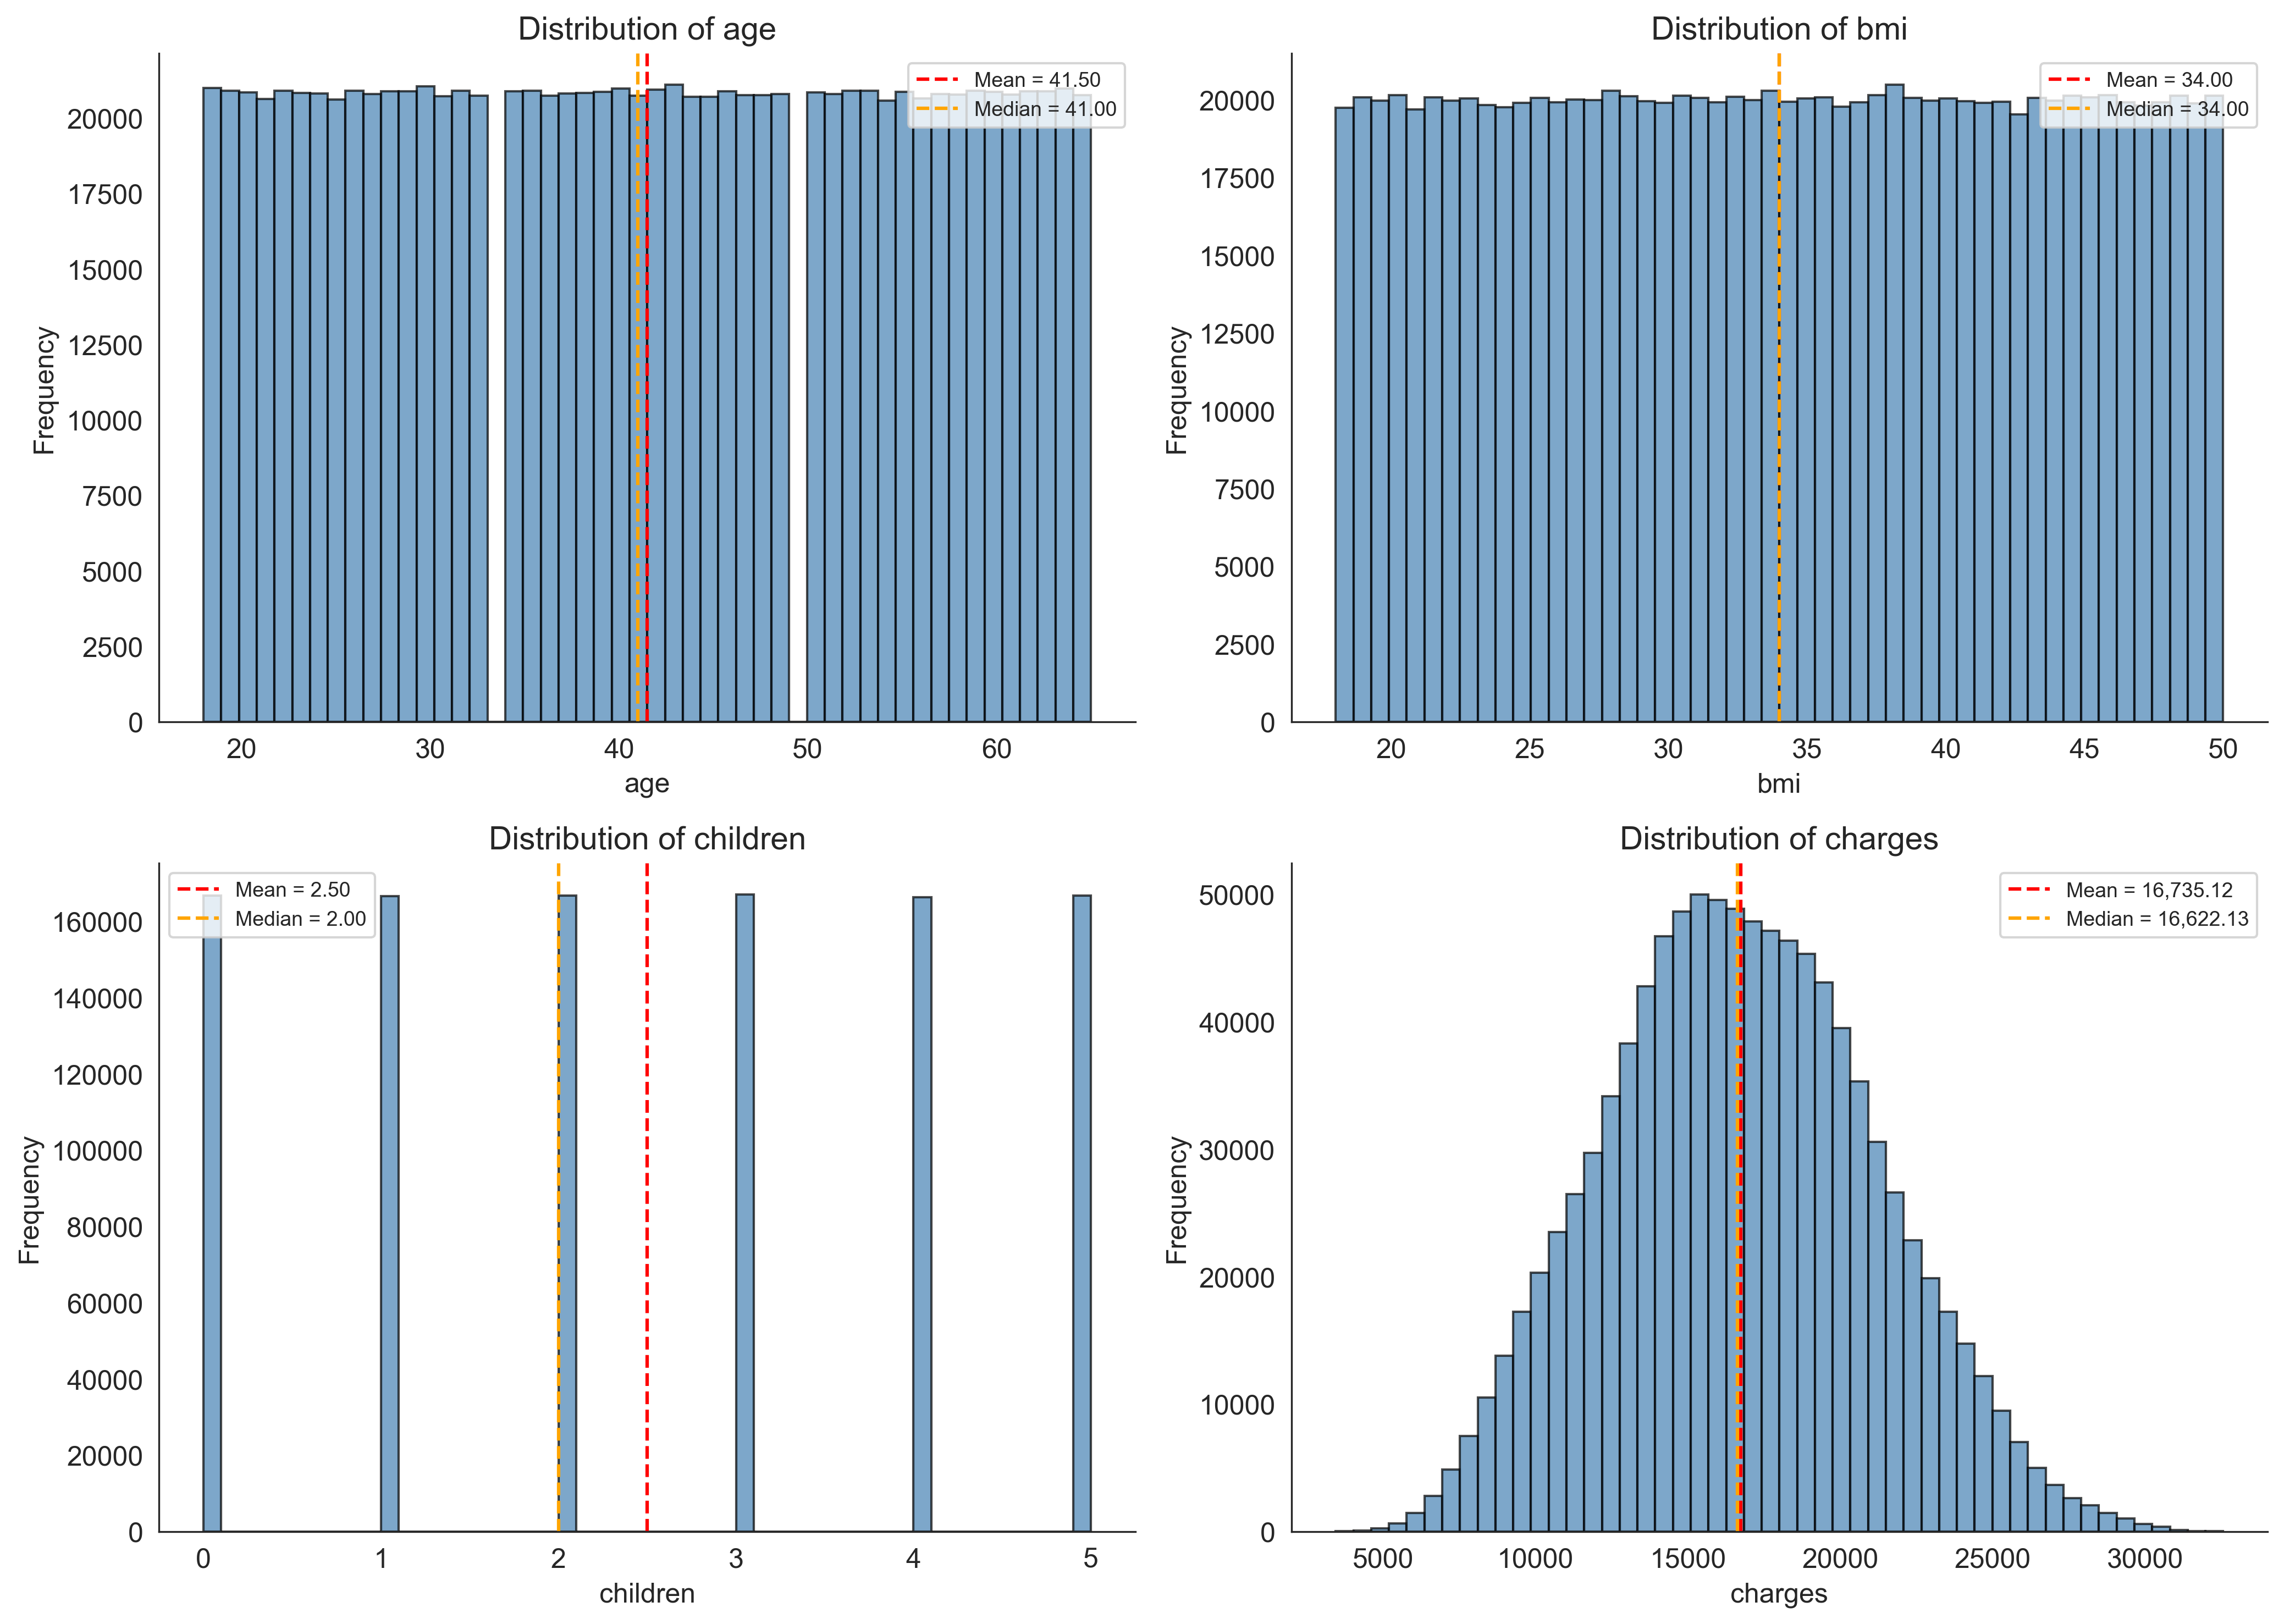
\includegraphics[width=0.90\textwidth]{Thesis/Chapter 3/Figures/fig_numeric_distributions.png}
\caption{Empirical distributions of the numerical variables.}
\label{fig:numeric_distributions}
\end{figure}

Selected percentiles of \texttt{charges} are reported in
Table~\ref{tab:charges_percentiles}.  The interquartile range is
approximately $6\,181$, and the 90th, 95th, and 99th percentiles are
$22\,591$, $24\,224$, and $27\,016$, respectively.  These values serve as
empirical scale references; in the later \gls{mc} and Shapley stages,
high-cost profiles are defined using upper-tail quantiles of the
simulated predicted-cost distribution, not directly from these observed
percentiles.

\begin{table}[H]
\centering
\small
\renewcommand{\arraystretch}{1.12}
\begin{tabular}{lrrrrrrrrr}
\toprule
\textbf{Percentile} & P1 & P5 & P10 & P25 & P50 & P75 & P90 & P95 & P99 \\
\midrule
\textbf{Value} &
7\,520 & 9\,558 & 10\,947 & 13\,600 & 16\,622 &
19\,781 & 22\,591 & 24\,224 & 27\,016 \\
\bottomrule
\end{tabular}
\caption{Selected percentiles of the response variable \texttt{charges}.}
\label{tab:charges_percentiles}
\end{table}

% ----------------------------
% 3.3.2 DEPENDENCE STRUCTURE
% ----------------------------

\subsubsection{Dependence structure}
The Pearson correlation matrix for the four numerical variables is given
in Table~\ref{tab:numeric_correlations}.

\begin{table}[H]
\centering
\small
\renewcommand{\arraystretch}{1.12}
\begin{tabular}{lrrrr}
\toprule
 & \texttt{age} & \texttt{bmi} & \texttt{children} & \texttt{charges} \\
\midrule
\texttt{age}      & 1.000 & 0.001 & $-0.001$ & 0.063 \\
\texttt{bmi}      & 0.001 & 1.000 & $-0.002$ & 0.104 \\
\texttt{children} & $-0.001$ & $-0.002$ & 1.000 & 0.077 \\
\texttt{charges}  & 0.063 & 0.104 & 0.077 & 1.000 \\
\bottomrule
\end{tabular}
\caption{Pearson correlation matrix for the numerical variables.}
\label{tab:numeric_correlations}
\end{table}

Pairwise correlations among the predictors are negligible
($|r| \le 0.002$), and the marginal correlations with \texttt{charges} are
weak.  This does not imply that the predictors are
unimportant (the deep
network can learn complex nonlinear interactions invisible to a linear
correlation matrix), but it does provide empirical support for the
product-marginal independence assumption used in the \gls{mc}
simulation.  The correlation heatmap in Figure~\ref{fig:correlation_heatmap}
confirms the uniformly pale off-diagonal shading.

\begin{figure}[H]
\centering
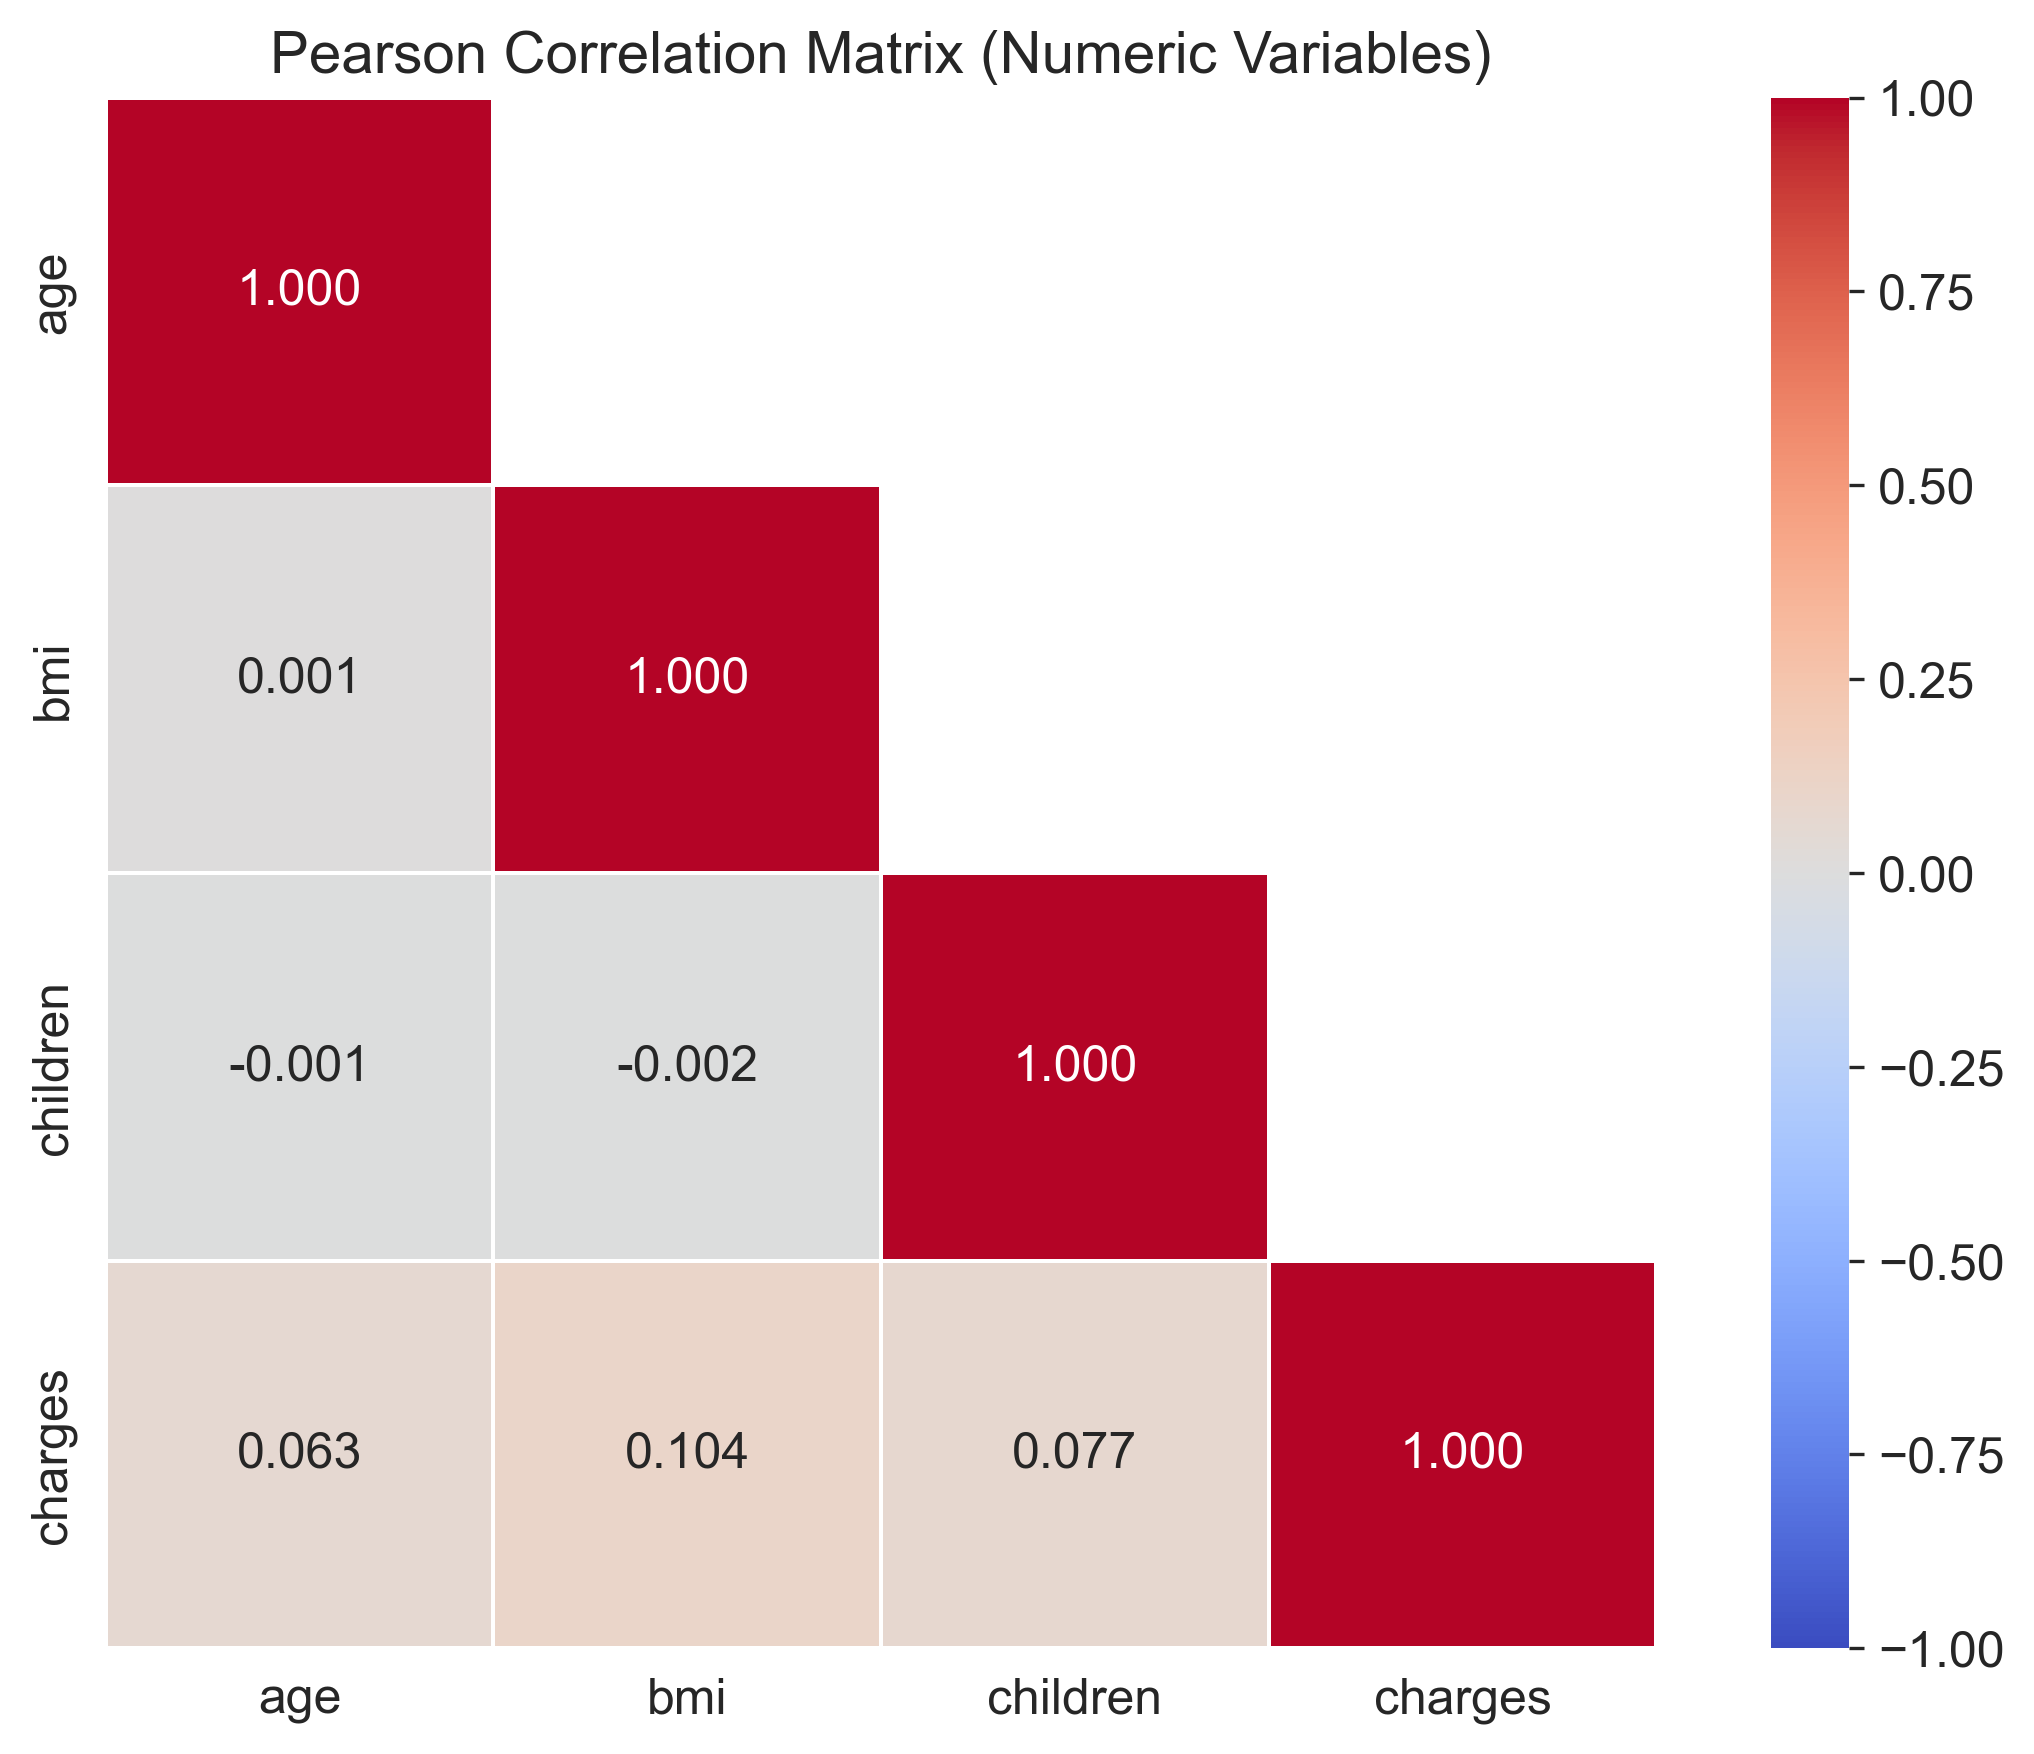
\includegraphics[width=0.60\textwidth]{Thesis/Chapter 3/Figures/fig_correlation_heatmap.png}
\caption{Pearson correlation heatmap for the numerical variables.}
\label{fig:correlation_heatmap}
\end{figure}

% ---------------------------------------------------
% 3.3.3 CATEGORICAL PREDICTORS AND ENCODED FEATURES
% ---------------------------------------------------

\subsubsection{Categorical predictors and encoded features}

\begin{figure}[H]
\centering
\begin{subfigure}[b]{\textwidth}
    \centering
    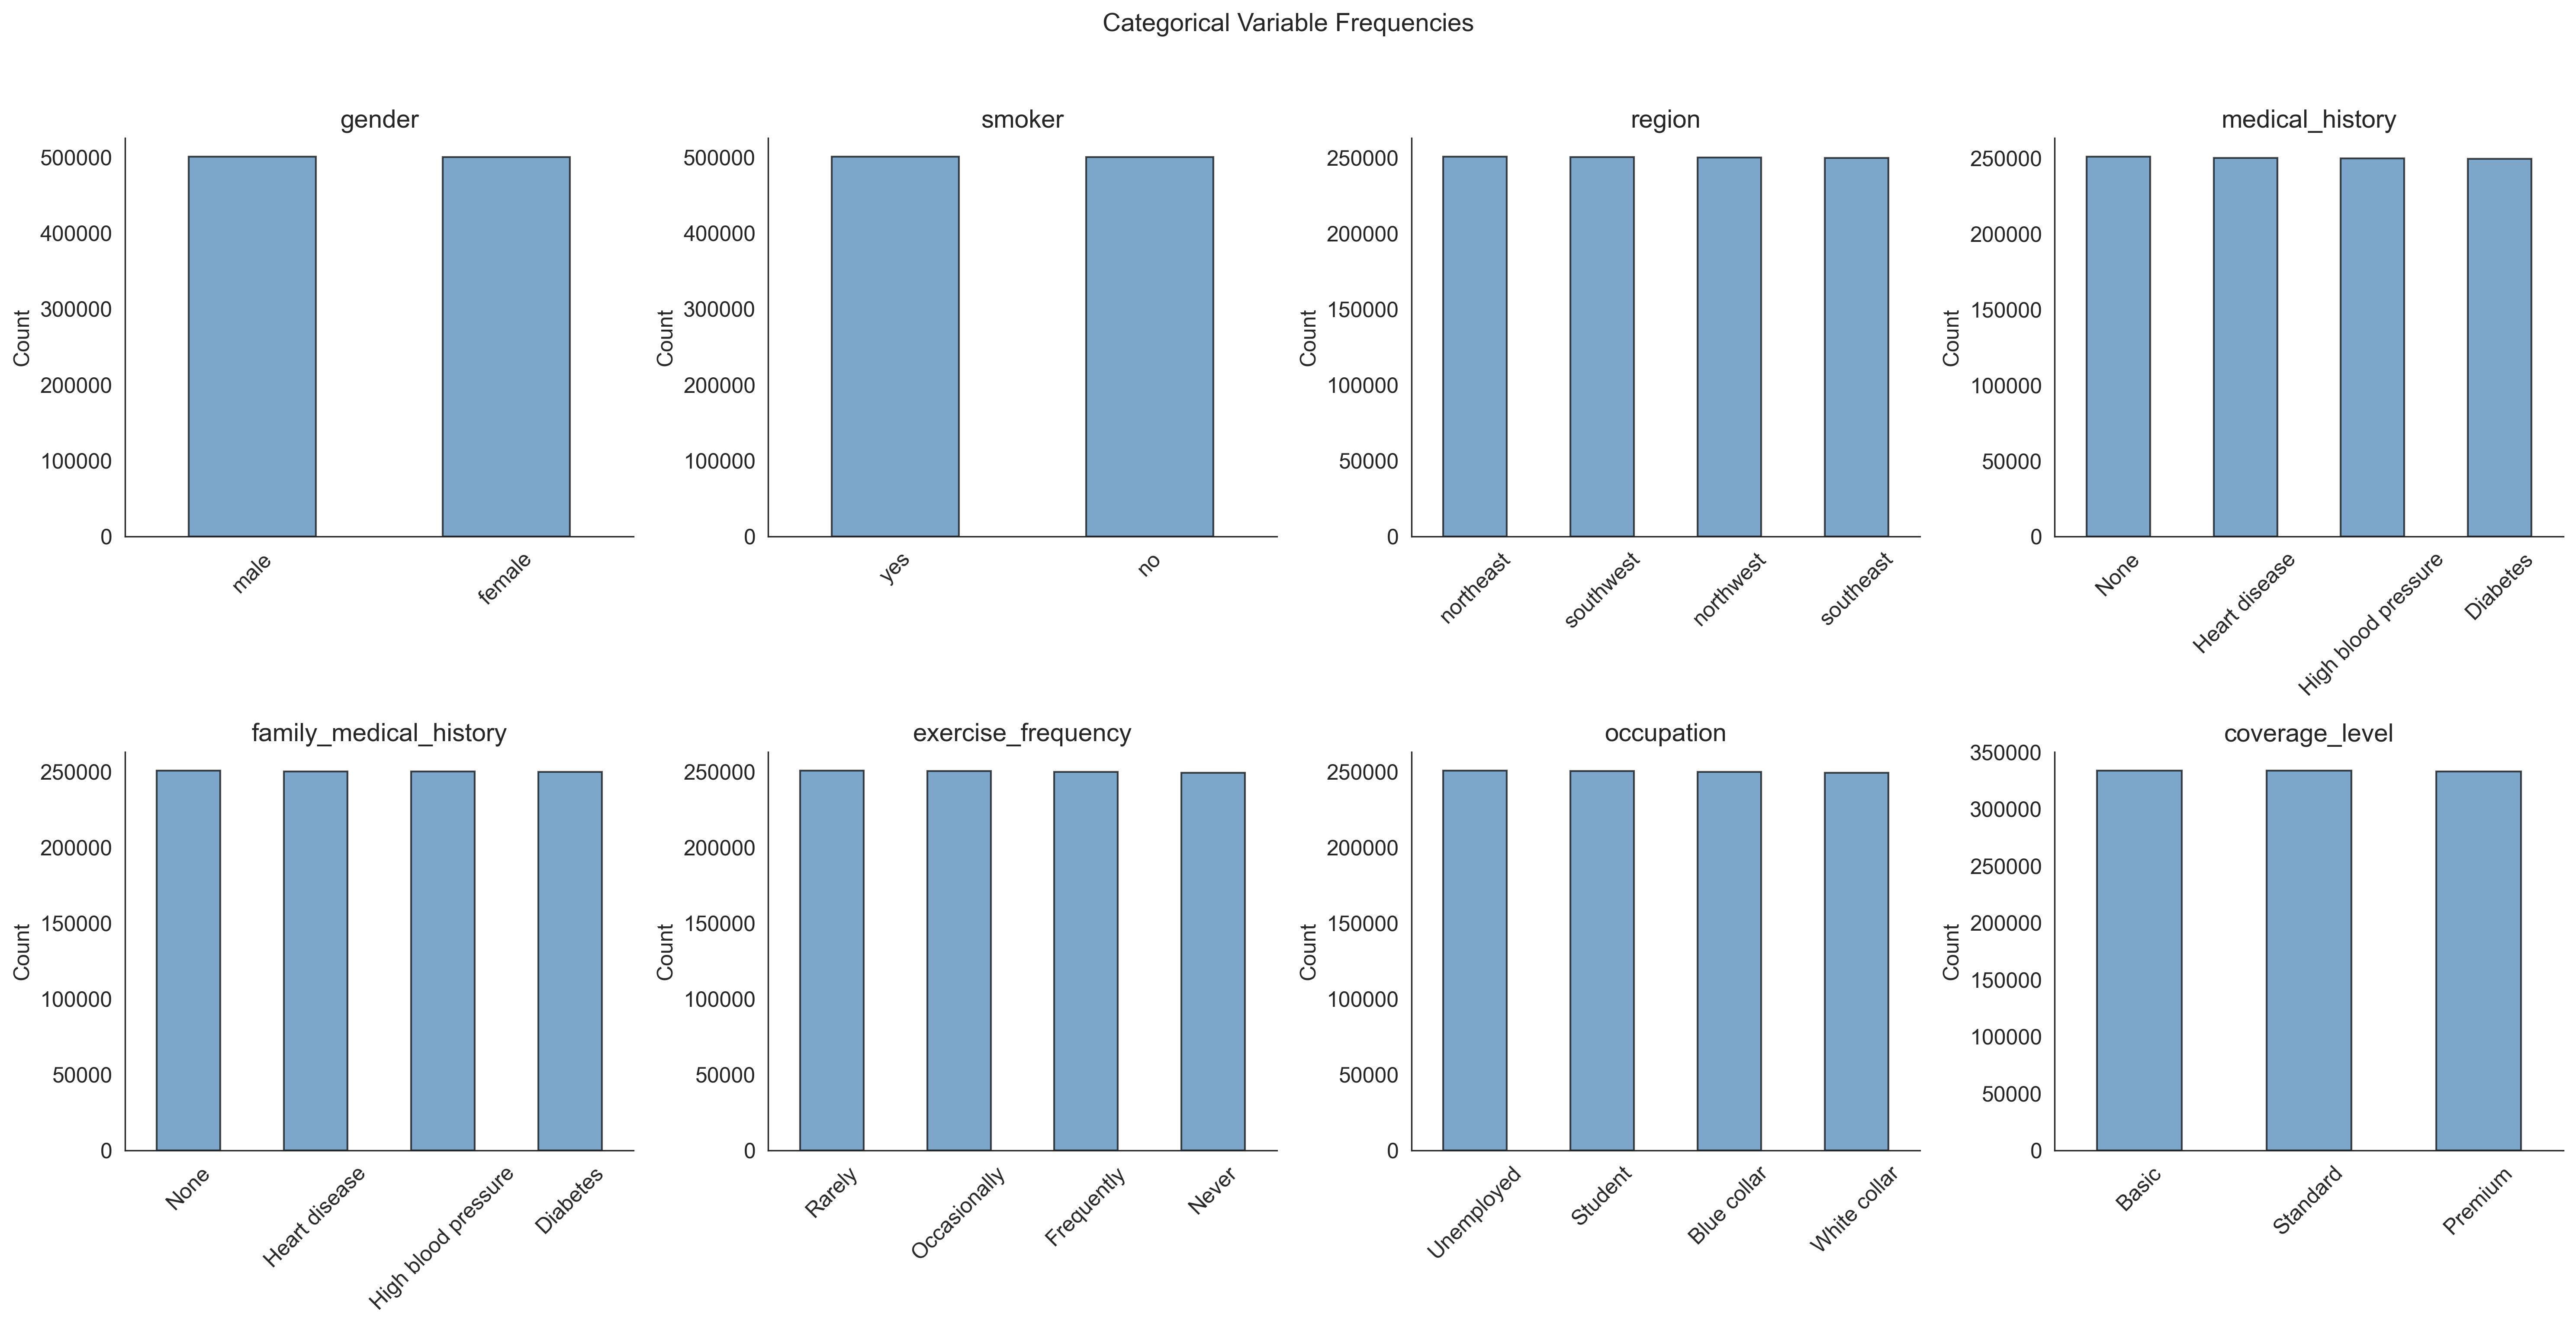
\includegraphics[width=0.95\textwidth]{Thesis/Chapter 3/Figures/fig_categorical_frequencies.png}
    \caption{Frequency distributions of categorical and binary predictors.}
    \label{fig:categorical_frequencies_ch3}
\end{subfigure}

\vspace{0.4cm}

\begin{subfigure}[b]{\textwidth}
    \centering
    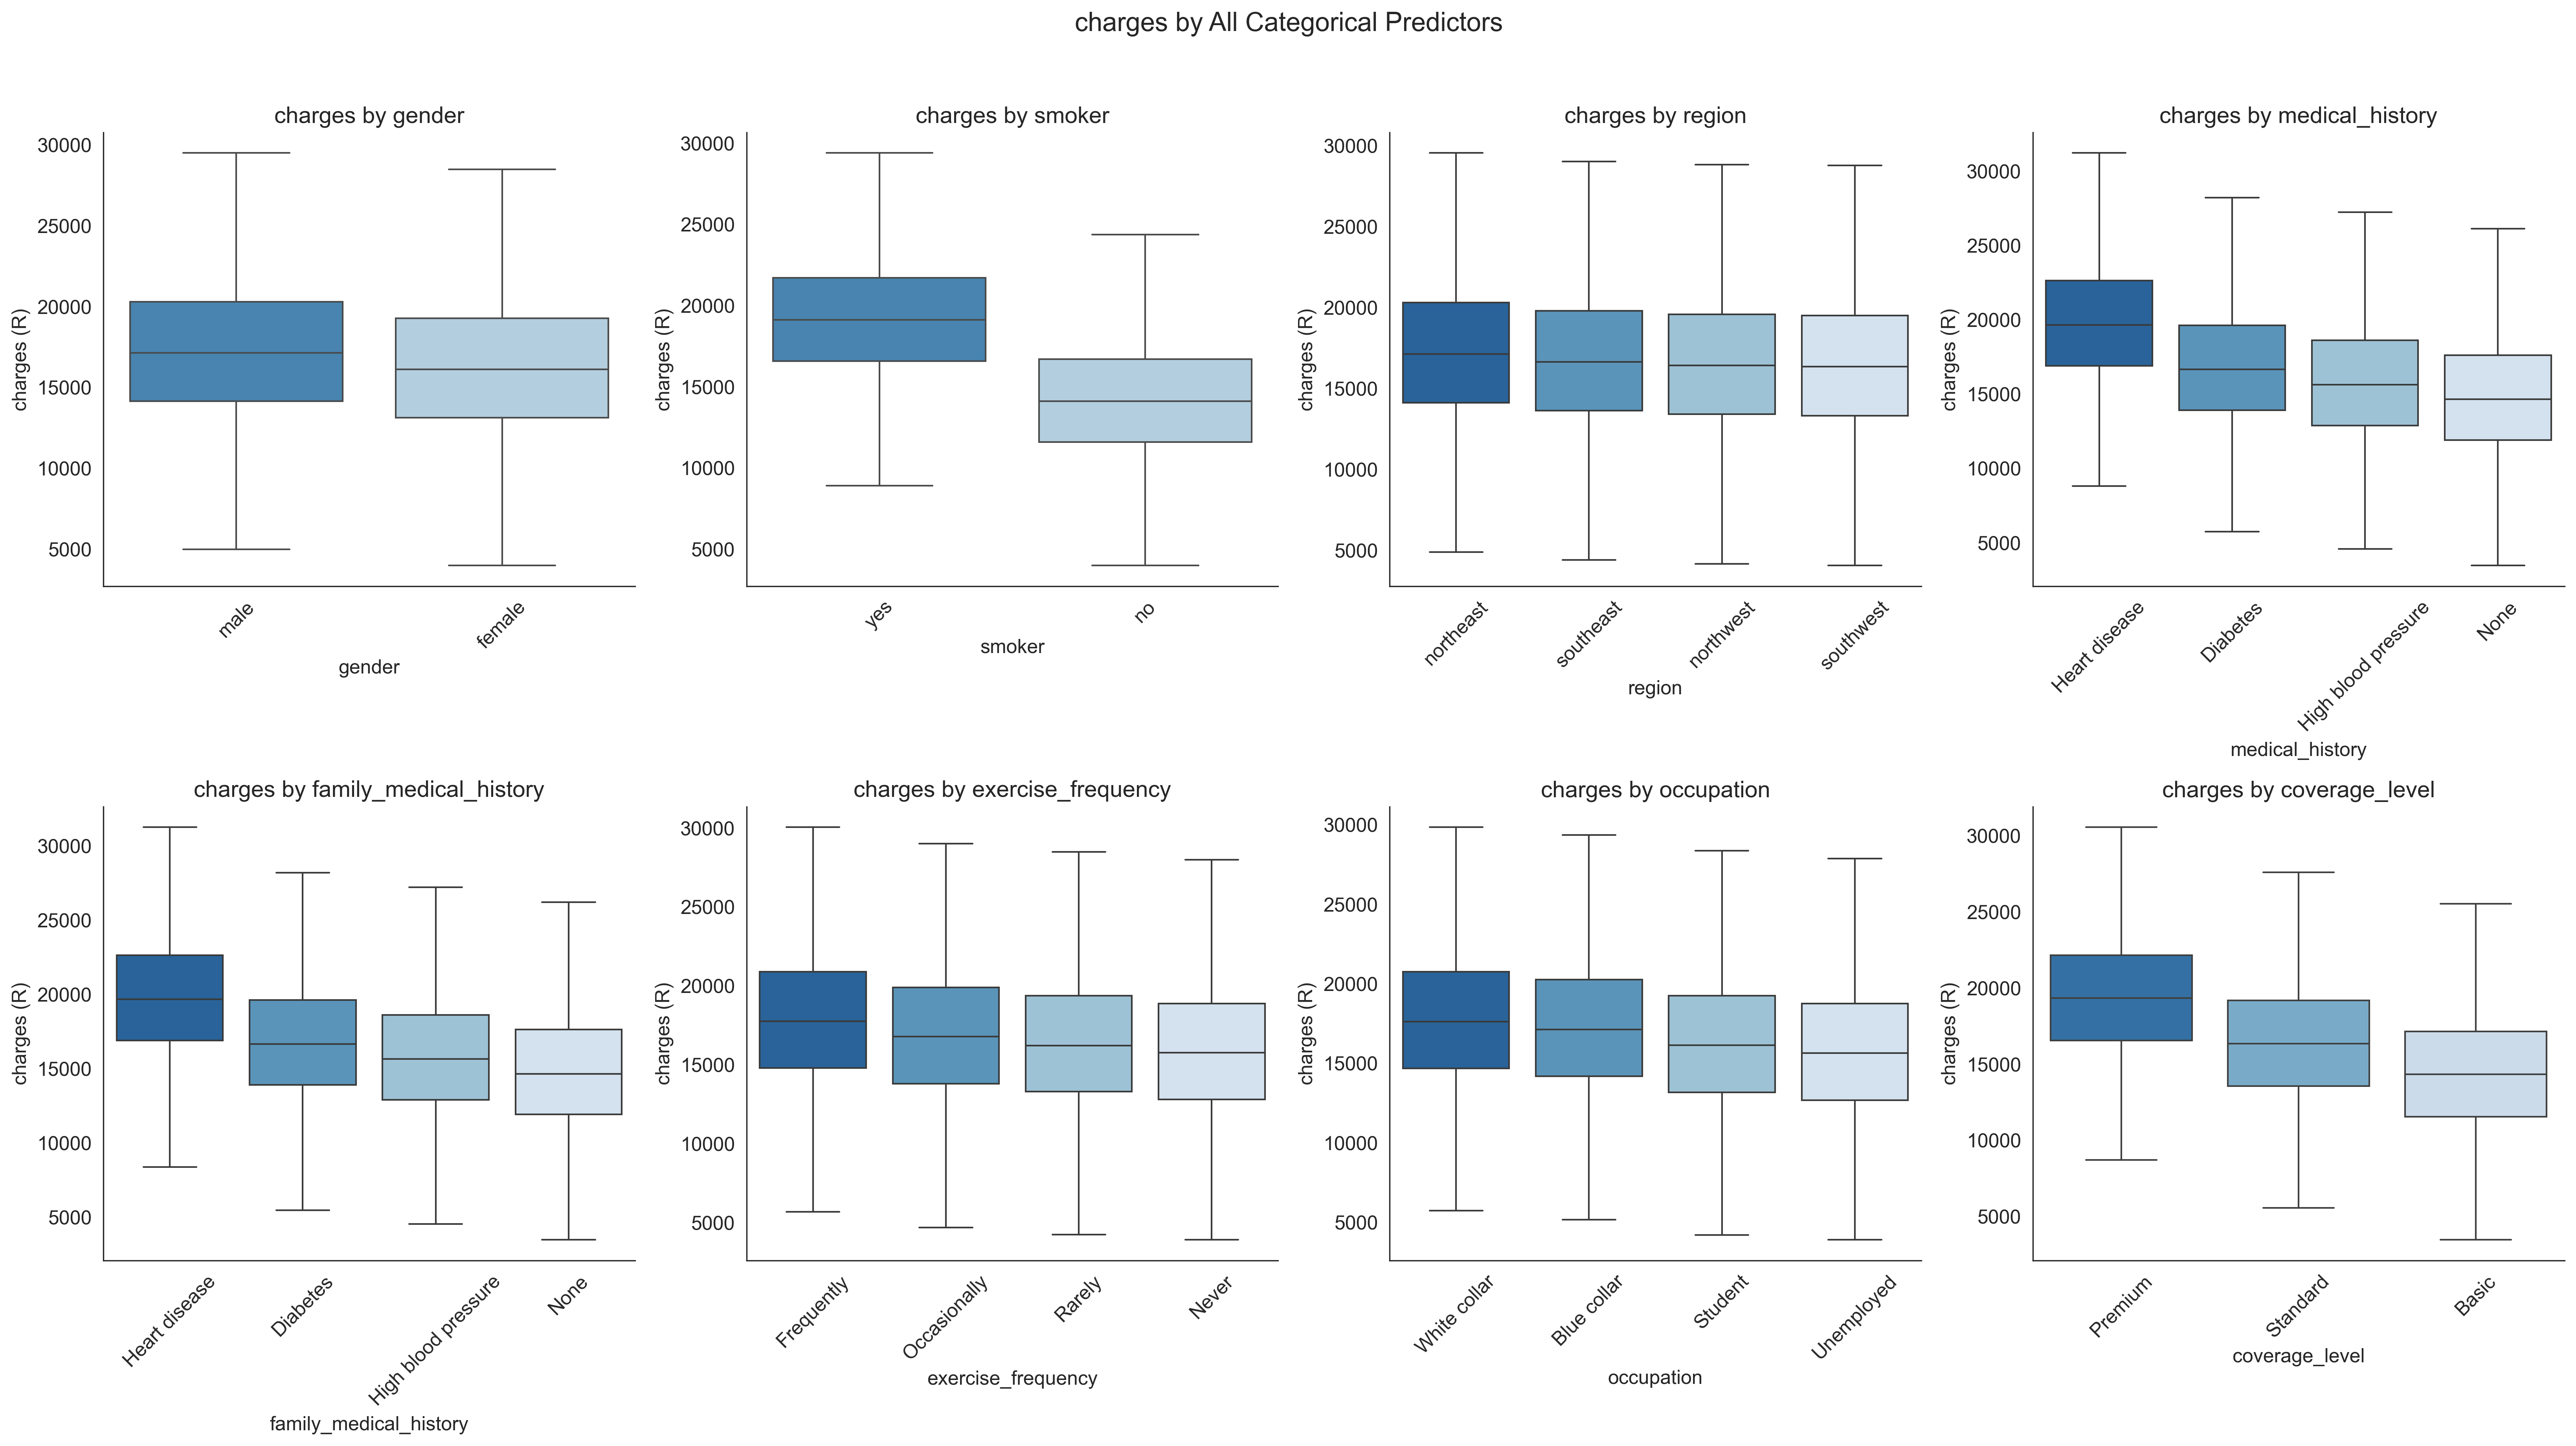
\includegraphics[width=0.95\textwidth]{Thesis/Chapter 3/Figures/fig_charges_by_all_categoricals.png}
    \caption{Boxplots of \texttt{charges} by categorical predictor.}
    \label{fig:charges_by_all_categoricals_ch3}
\end{subfigure}
\caption{Categorical predictor diagnostics: frequency distributions and conditional boxplots.}
\label{fig:categorical_diagnostics_ch3}
\end{figure}

\noindent
Figure~\ref{fig:categorical_frequencies_ch3} confirms that every
categorical and binary predictor is approximately uniformly distributed
across its levels. The two binary variables (\texttt{gender} and
\texttt{smoker}) each have close to 500\,000 observations per level, the
four-level variables (\texttt{region},\allowbreak{}
\texttt{medical\_\allowbreak{}history},\allowbreak{}
\texttt{family\_medical\_\allowbreak{}history},\allowbreak{}
\texttt{exercise\_\allowbreak{}frequency} and
\texttt{occupation}) each have approximately 250\,000 observations per
level, and the three-level \texttt{coverage\_\allowbreak{}level} variable has
approximately 333\,000 observations per tier. These balanced frequencies
ensure that no category is underrepresented in the training data and that
the fitted category proportions used in the \gls{mc} simulation are
estimated with high precision.

Figure~\ref{fig:charges_by_all_categoricals_ch3} displays the conditional
distribution of charges for each categorical predictor. The
\texttt{smoker} panel shows the clearest separation: smokers have a median
near R19\,000 compared to approximately R14\,000 for non-smokers. The
\texttt{coverage\_\allowbreak{}level} panel reveals a monotonic tier structure, with
Premium policyholders having the highest median charges (approximately
R20\,000), followed by Standard (approximately R17\,000) and Basic
(approximately R15\,000). Among \texttt{medical\_\allowbreak{}history} categories,
Heart disease is associated with the highest median charges (approximately
R20\,000), followed by Diabetes, High blood pressure and None. The
\texttt{family\_medical\_\allowbreak{}history} panel shows the same ordering, with Heart
disease again yielding the highest charges. The \texttt{exercise\_\allowbreak{}frequency}
panel shows a modest gradient, with Frequently exercising policyholders
having marginally higher median charges than those who Never exercise.
The \texttt{gender}, \texttt{region} and \texttt{occupation} panels display
smaller unconditional differences, though males tend to have slightly
higher charges than females across all panels.

Two-way interactions were examined for
\texttt{smoker}~$\times$~\texttt{coverage\_\allowbreak{}level},
\texttt{smoker}~$\times$~\texttt{medical\_\allowbreak{}history} and
\texttt{coverage\_\allowbreak{}level}~$\times$~\texttt{gender} to assess whether the
effect of one variable on charges depends on the level of another.

\begin{figure}[H]
\centering
\begin{subfigure}[b]{\textwidth}
    \centering
    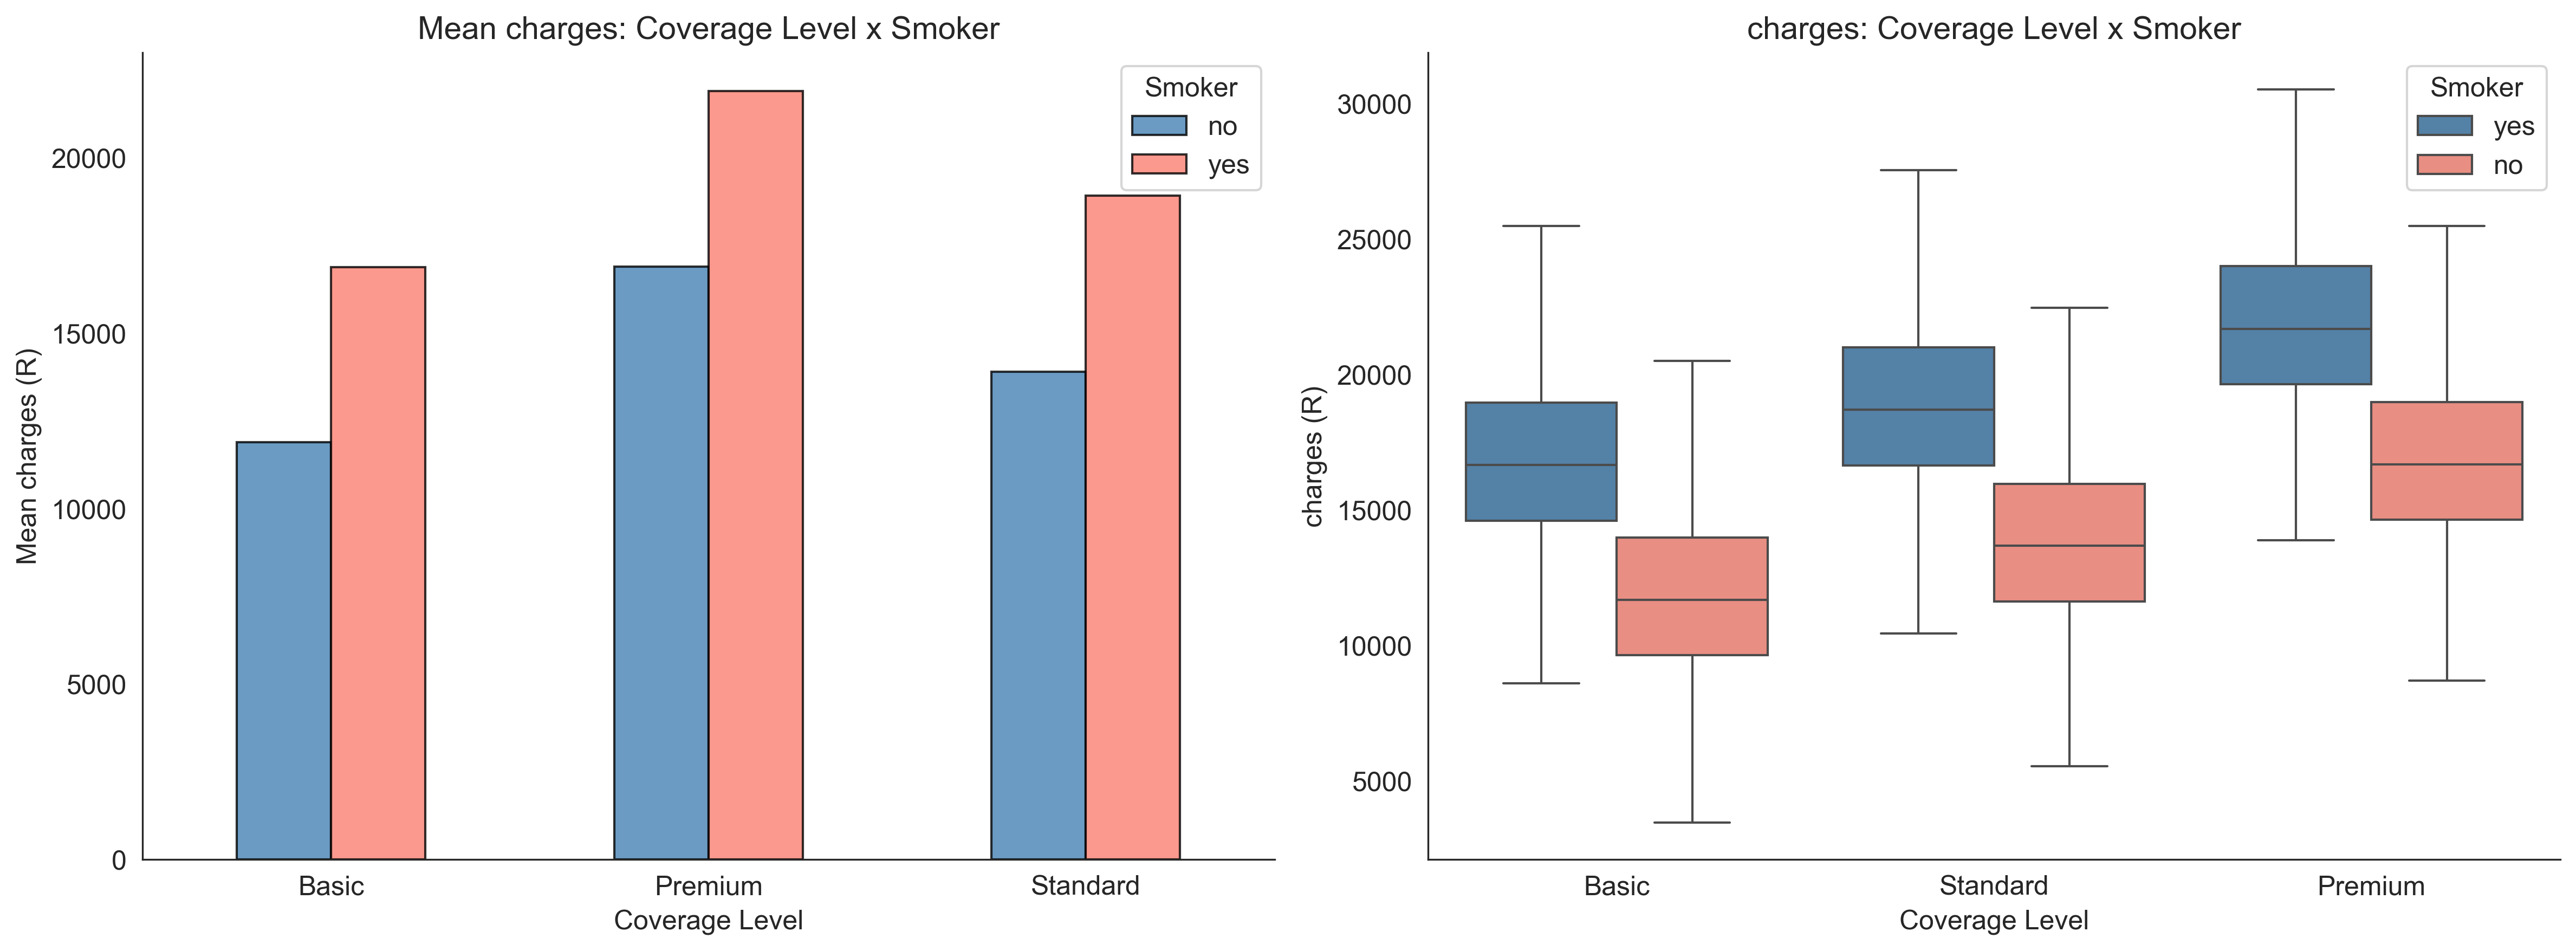
\includegraphics[width=0.95\textwidth]{Thesis/Chapter 3/Figures/fig_interaction_smoker_coverage.png}
    \caption{\texttt{smoker}~$\times$~\texttt{coverage\_\allowbreak{}level} interaction effects on charges.}
    \label{fig:interaction_smoker_coverage_ch3}
\end{subfigure}

\vspace{0.3cm}

\begin{subfigure}[b]{\textwidth}
    \centering
    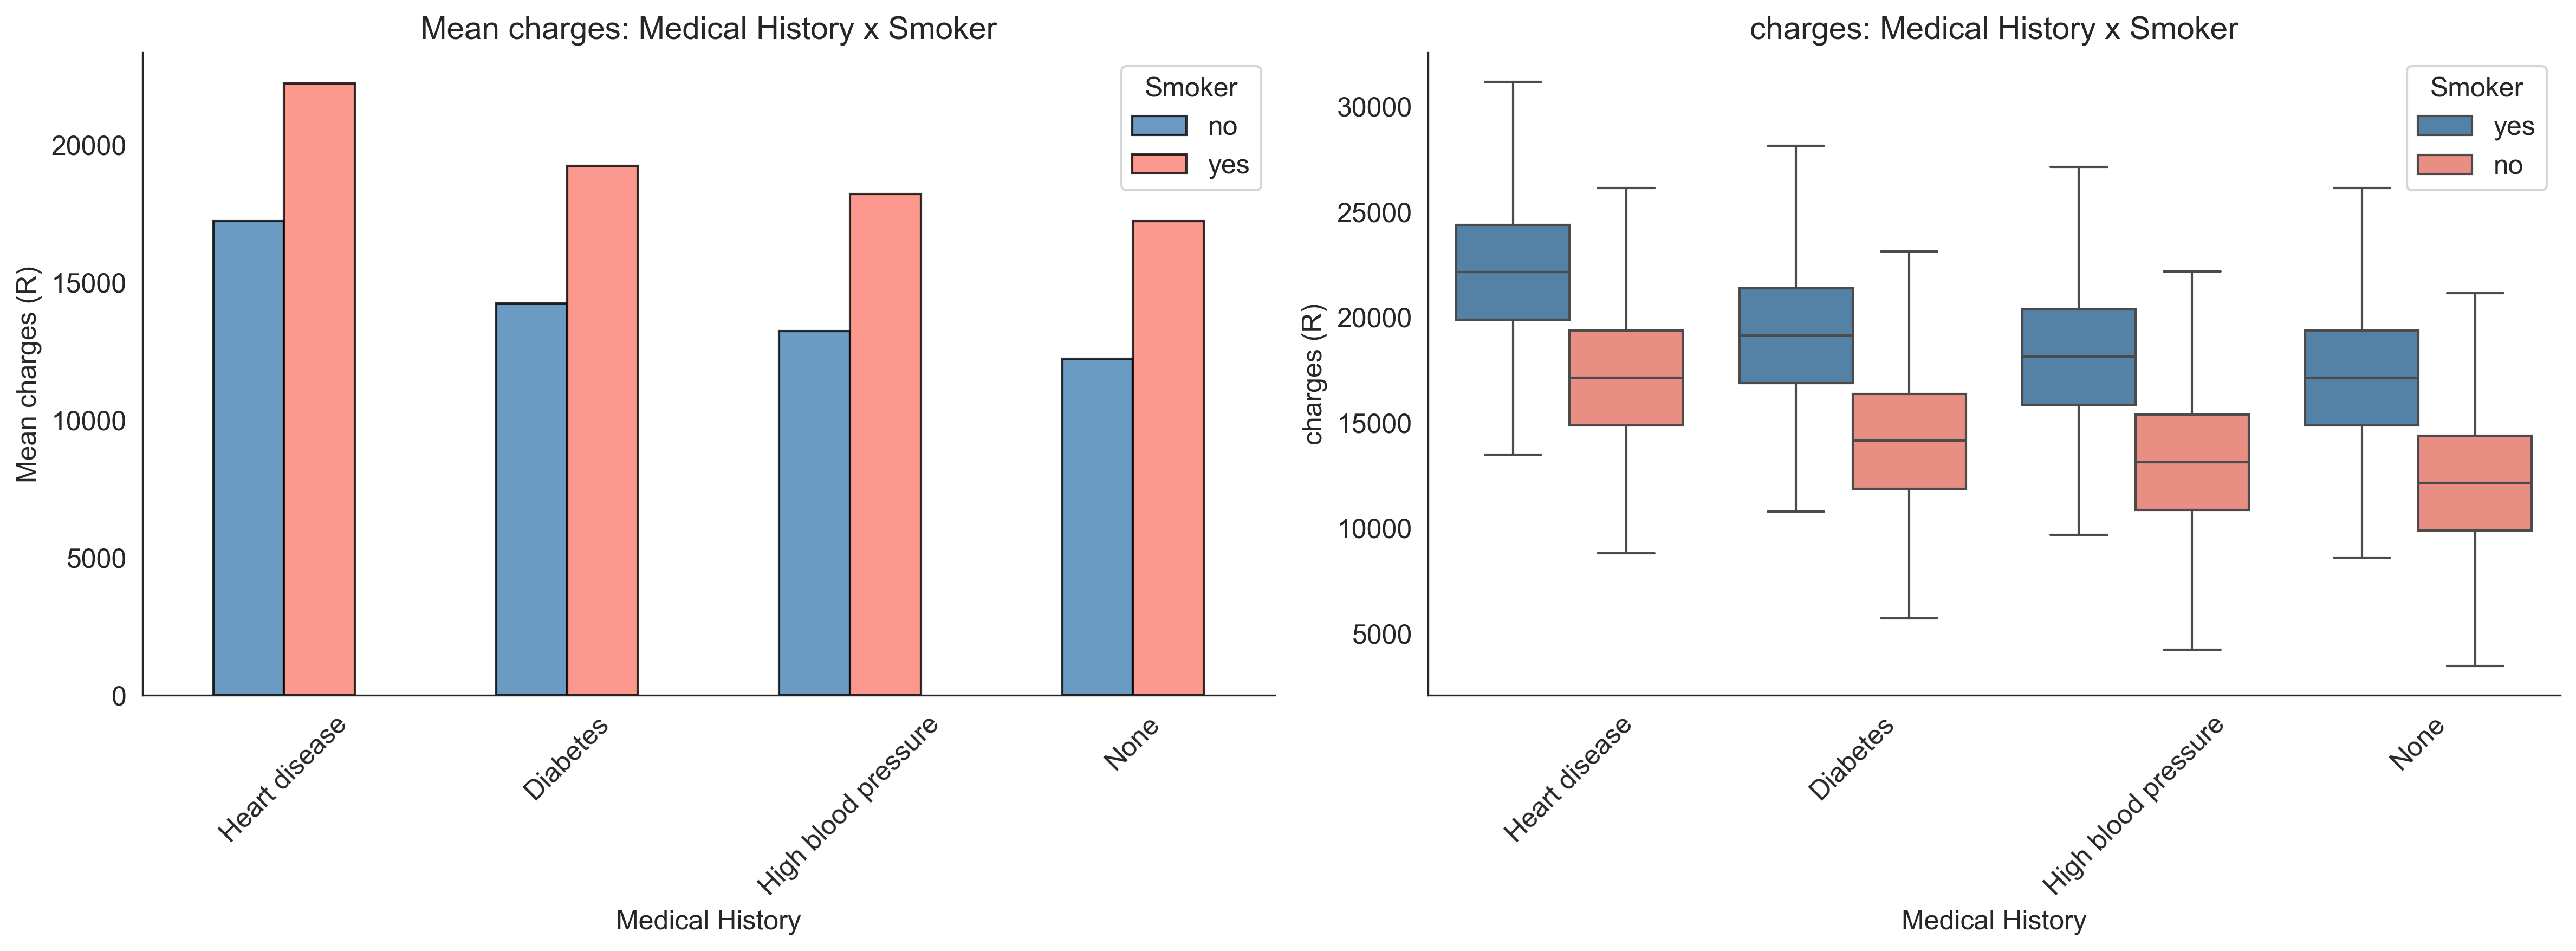
\includegraphics[width=0.95\textwidth]{Thesis/Chapter 3/Figures/fig_interaction_smoker_medical.png}
    \caption{\texttt{smoker}~$\times$~\texttt{medical\_\allowbreak{}history} interaction effects on charges.}
    \label{fig:interaction_smoker_medical_ch3}
\end{subfigure}

\vspace{0.3cm}

\begin{subfigure}[b]{0.65\textwidth}
    \centering
    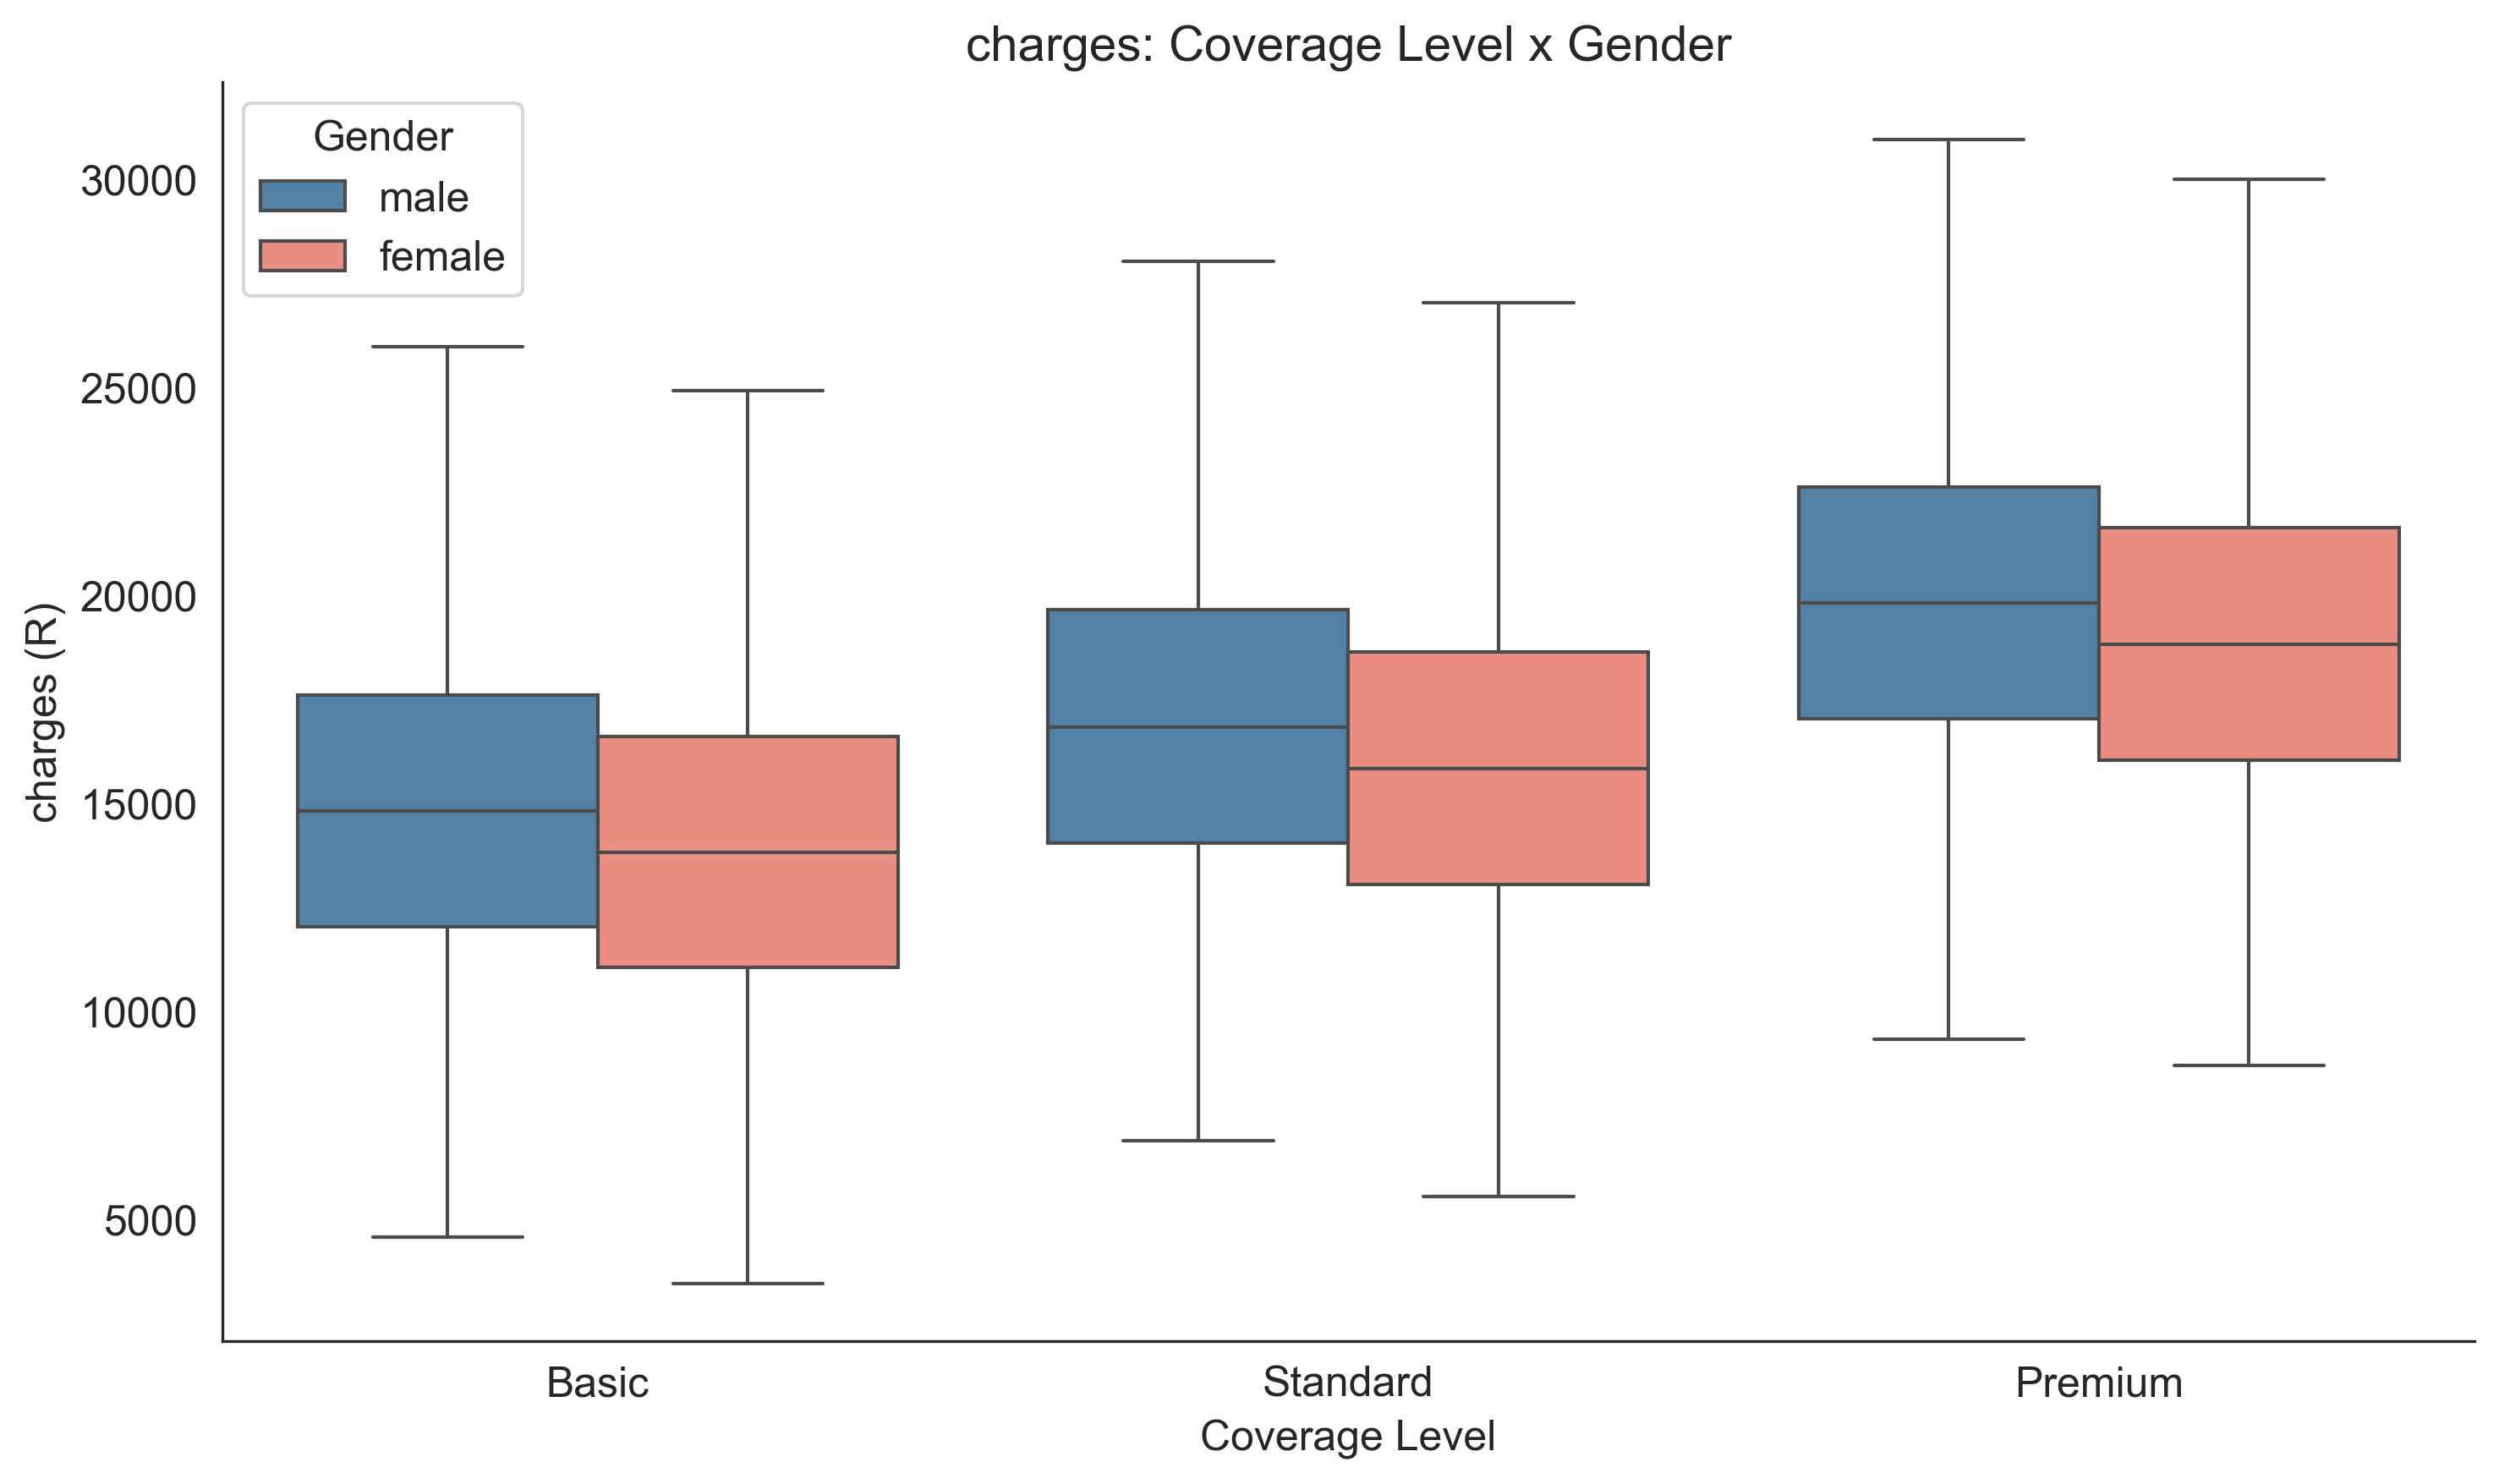
\includegraphics[width=\textwidth]{Thesis/Chapter 3/Figures/fig_interaction_coverage_gender.png}
    \caption{\texttt{coverage\_\allowbreak{}level}~$\times$~\texttt{gender} interaction effects on charges.}
    \label{fig:interaction_coverage_gender_ch3}
\end{subfigure}
\caption{Two-way interaction effects on \texttt{charges}.}
\label{fig:interaction_effects_ch3}
\end{figure}

\noindent
Figure~\ref{fig:interaction_smoker_coverage_ch3} shows that the smoker
effect is present at every coverage tier but is amplified at higher
coverage levels. At the Basic tier, the difference in mean charges between
smokers and non-smokers is approximately R5\,000 (R17\,000 versus R12\,000), whereas
at the Premium tier the difference widens to approximately R5\,000 to R6\,000
on a higher base (R22\,000 versus R17\,000). The boxplots confirm that
smokers consistently occupy a higher distributional range within each tier.
Figure~\ref{fig:interaction_smoker_medical_ch3} reveals a consistent
smoker premium across all medical history categories. The largest combined
effect occurs for smokers with Heart disease (mean charges approximately
R22\,500), while the lowest occurs for non-smokers with no reported
condition (approximately R12\,500). The smoker effect (approximately
R5\,000) is additive with the medical history effect, with the gap
remaining relatively stable across all four levels.
Figure~\ref{fig:interaction_coverage_gender_ch3} shows that males have
slightly higher median charges than females at every coverage tier, with
the gender gap widening modestly from Basic (approximately R1\,000) to
Premium (approximately R1\,500). The interaction effects visible in
Figure~\ref{fig:interaction_effects_ch3} support the use of a flexible \gls{dnn}
architecture capable of capturing nonlinear and interaction-based
relationships.

After encoding, the Pearson correlations between the 22 encoded predictors
and \texttt{charges} were computed on the training partition. The strongest
linear associations are \texttt{smoker} ($r = 0.567$),\allowbreak{}
\texttt{coverage\_level\_\allowbreak{}Premium} ($r = 0.427$),\allowbreak{}
\texttt{medical\_history\_\allowbreak{}Heart\_disease} ($r = 0.393$) and
\texttt{family\_medical\_\allowbreak{}history\_\allowbreak{}Heart\_disease} ($r = 0.393$).

\begin{figure}[H]
\centering
\begin{subfigure}[b]{0.48\textwidth}
    \centering
    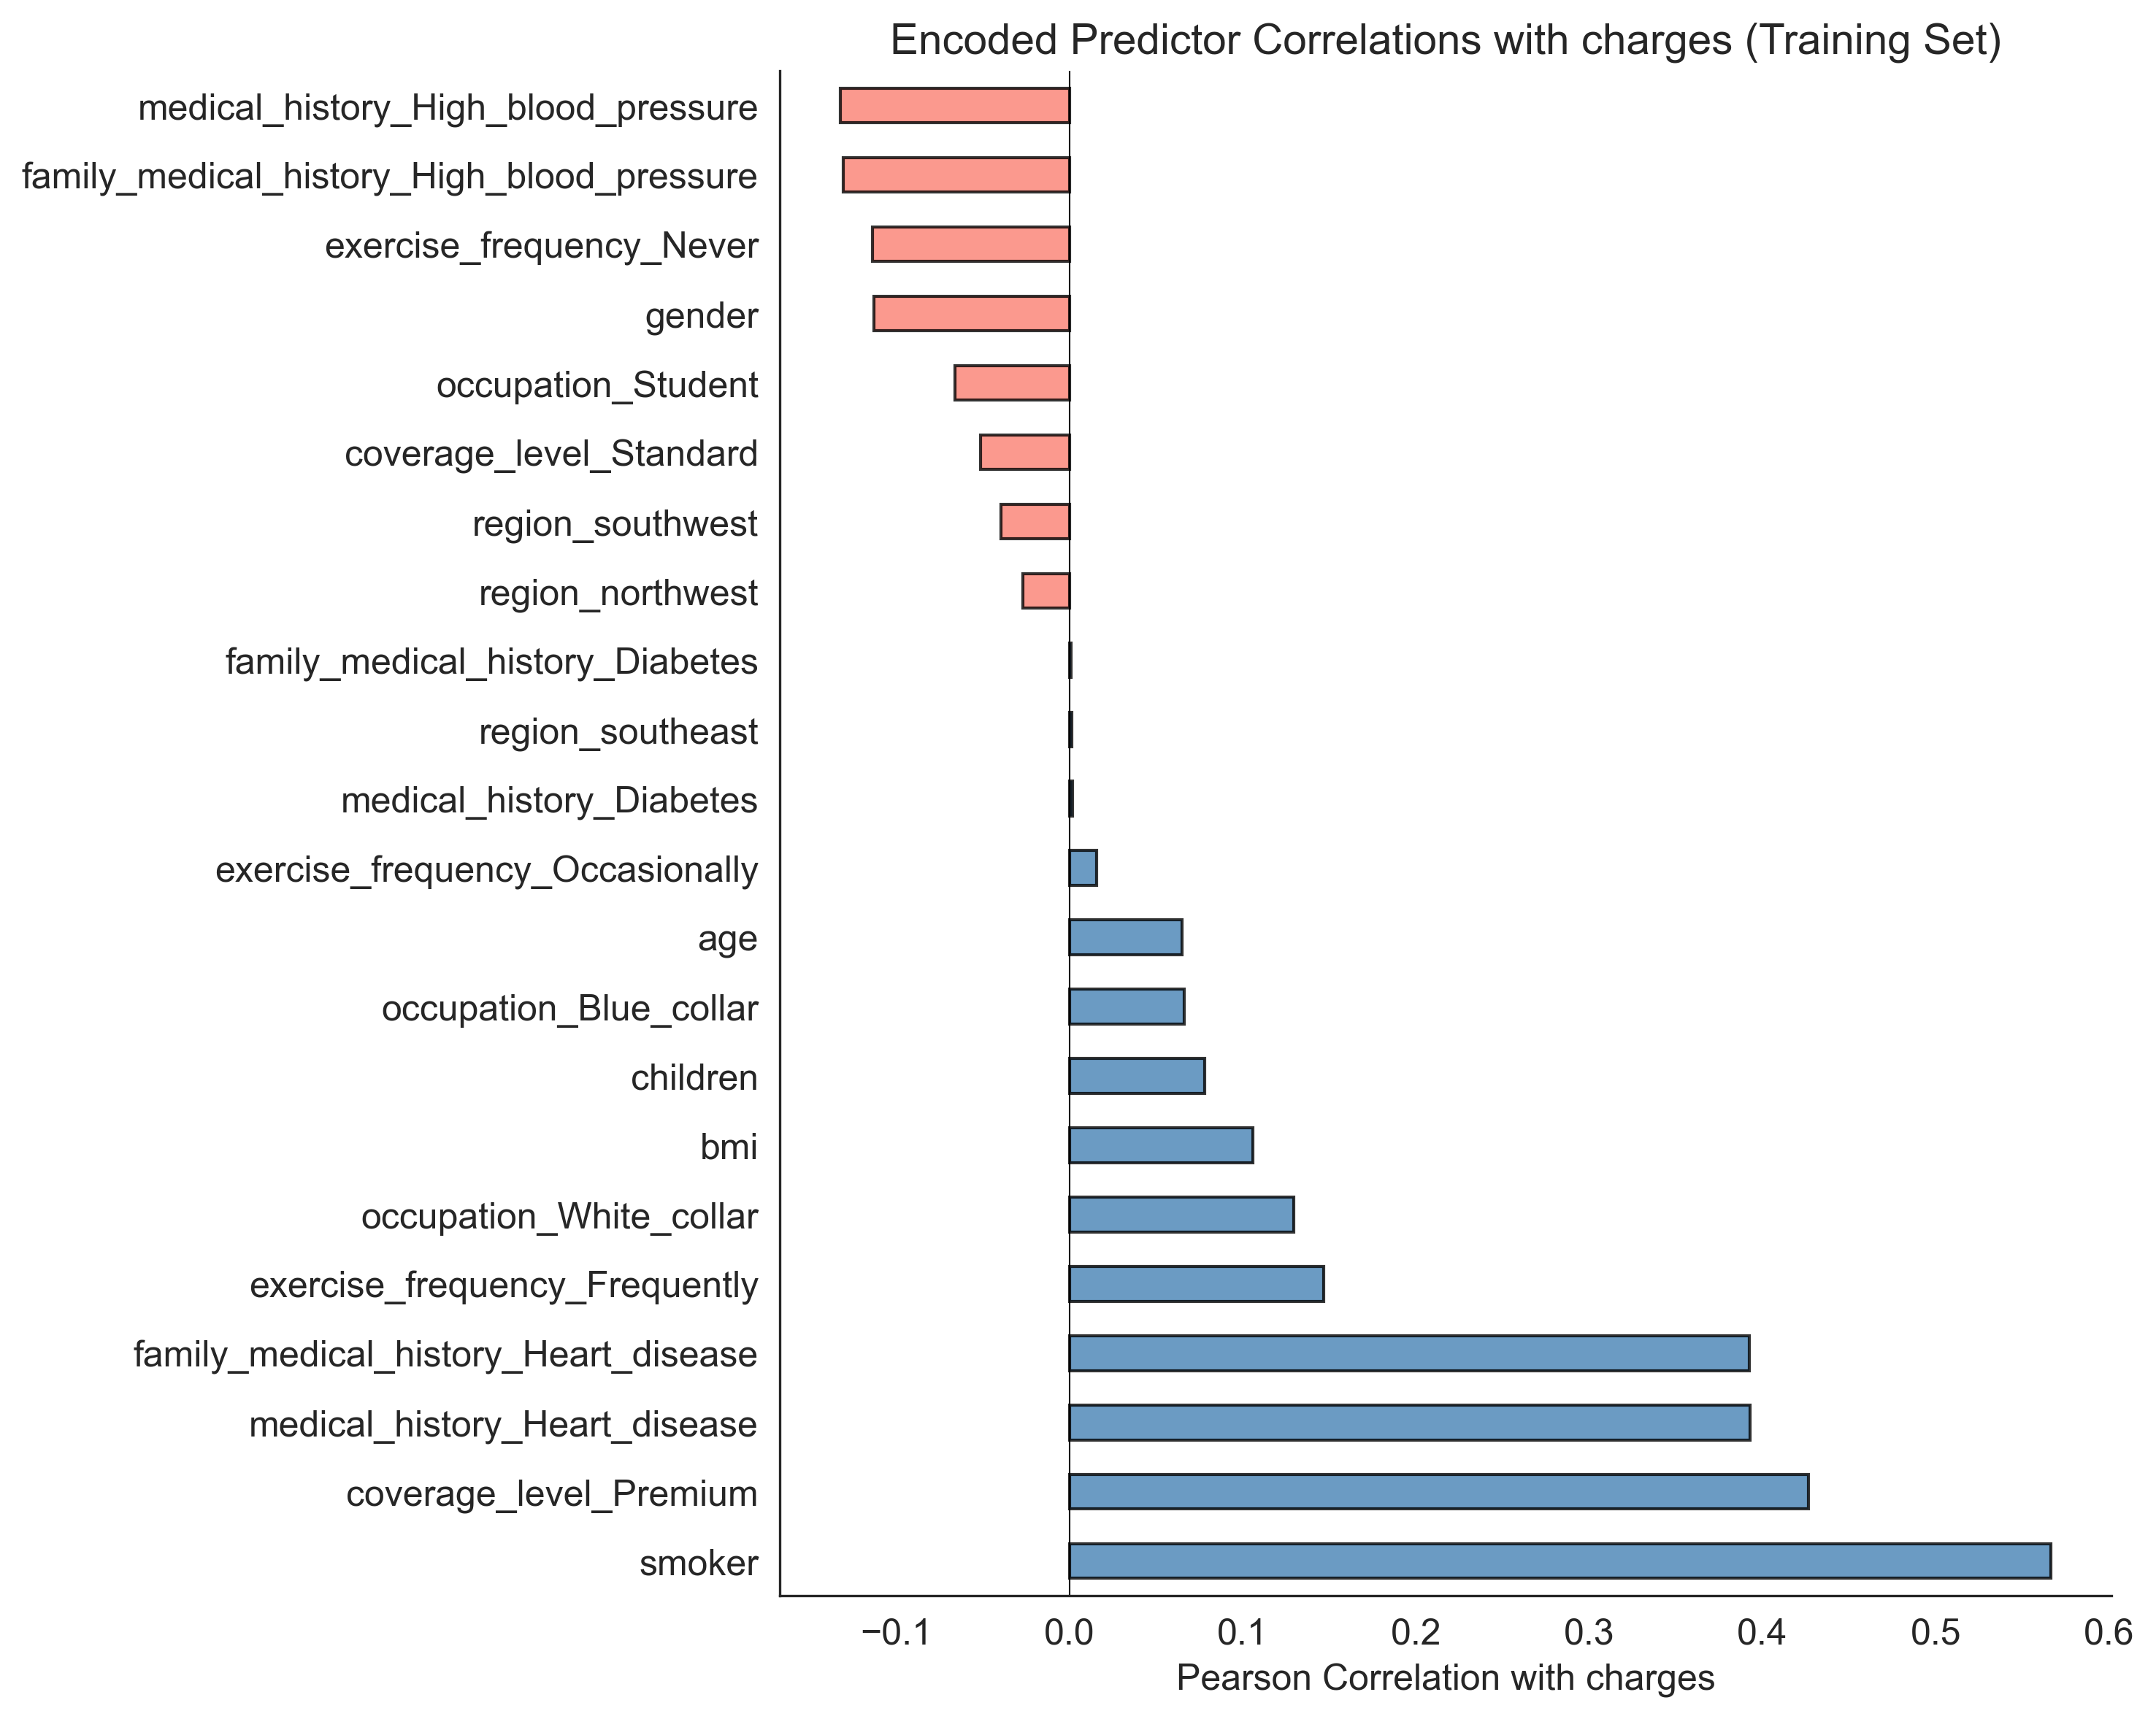
\includegraphics[width=\textwidth]{Thesis/Chapter 3/Figures/fig_encoded_correlations.png}
    \caption{Pearson correlations of encoded predictors with \texttt{charges}.}
    \label{fig:encoded_correlations_ch3}
\end{subfigure}
\hfill
\begin{subfigure}[b]{0.48\textwidth}
    \centering
    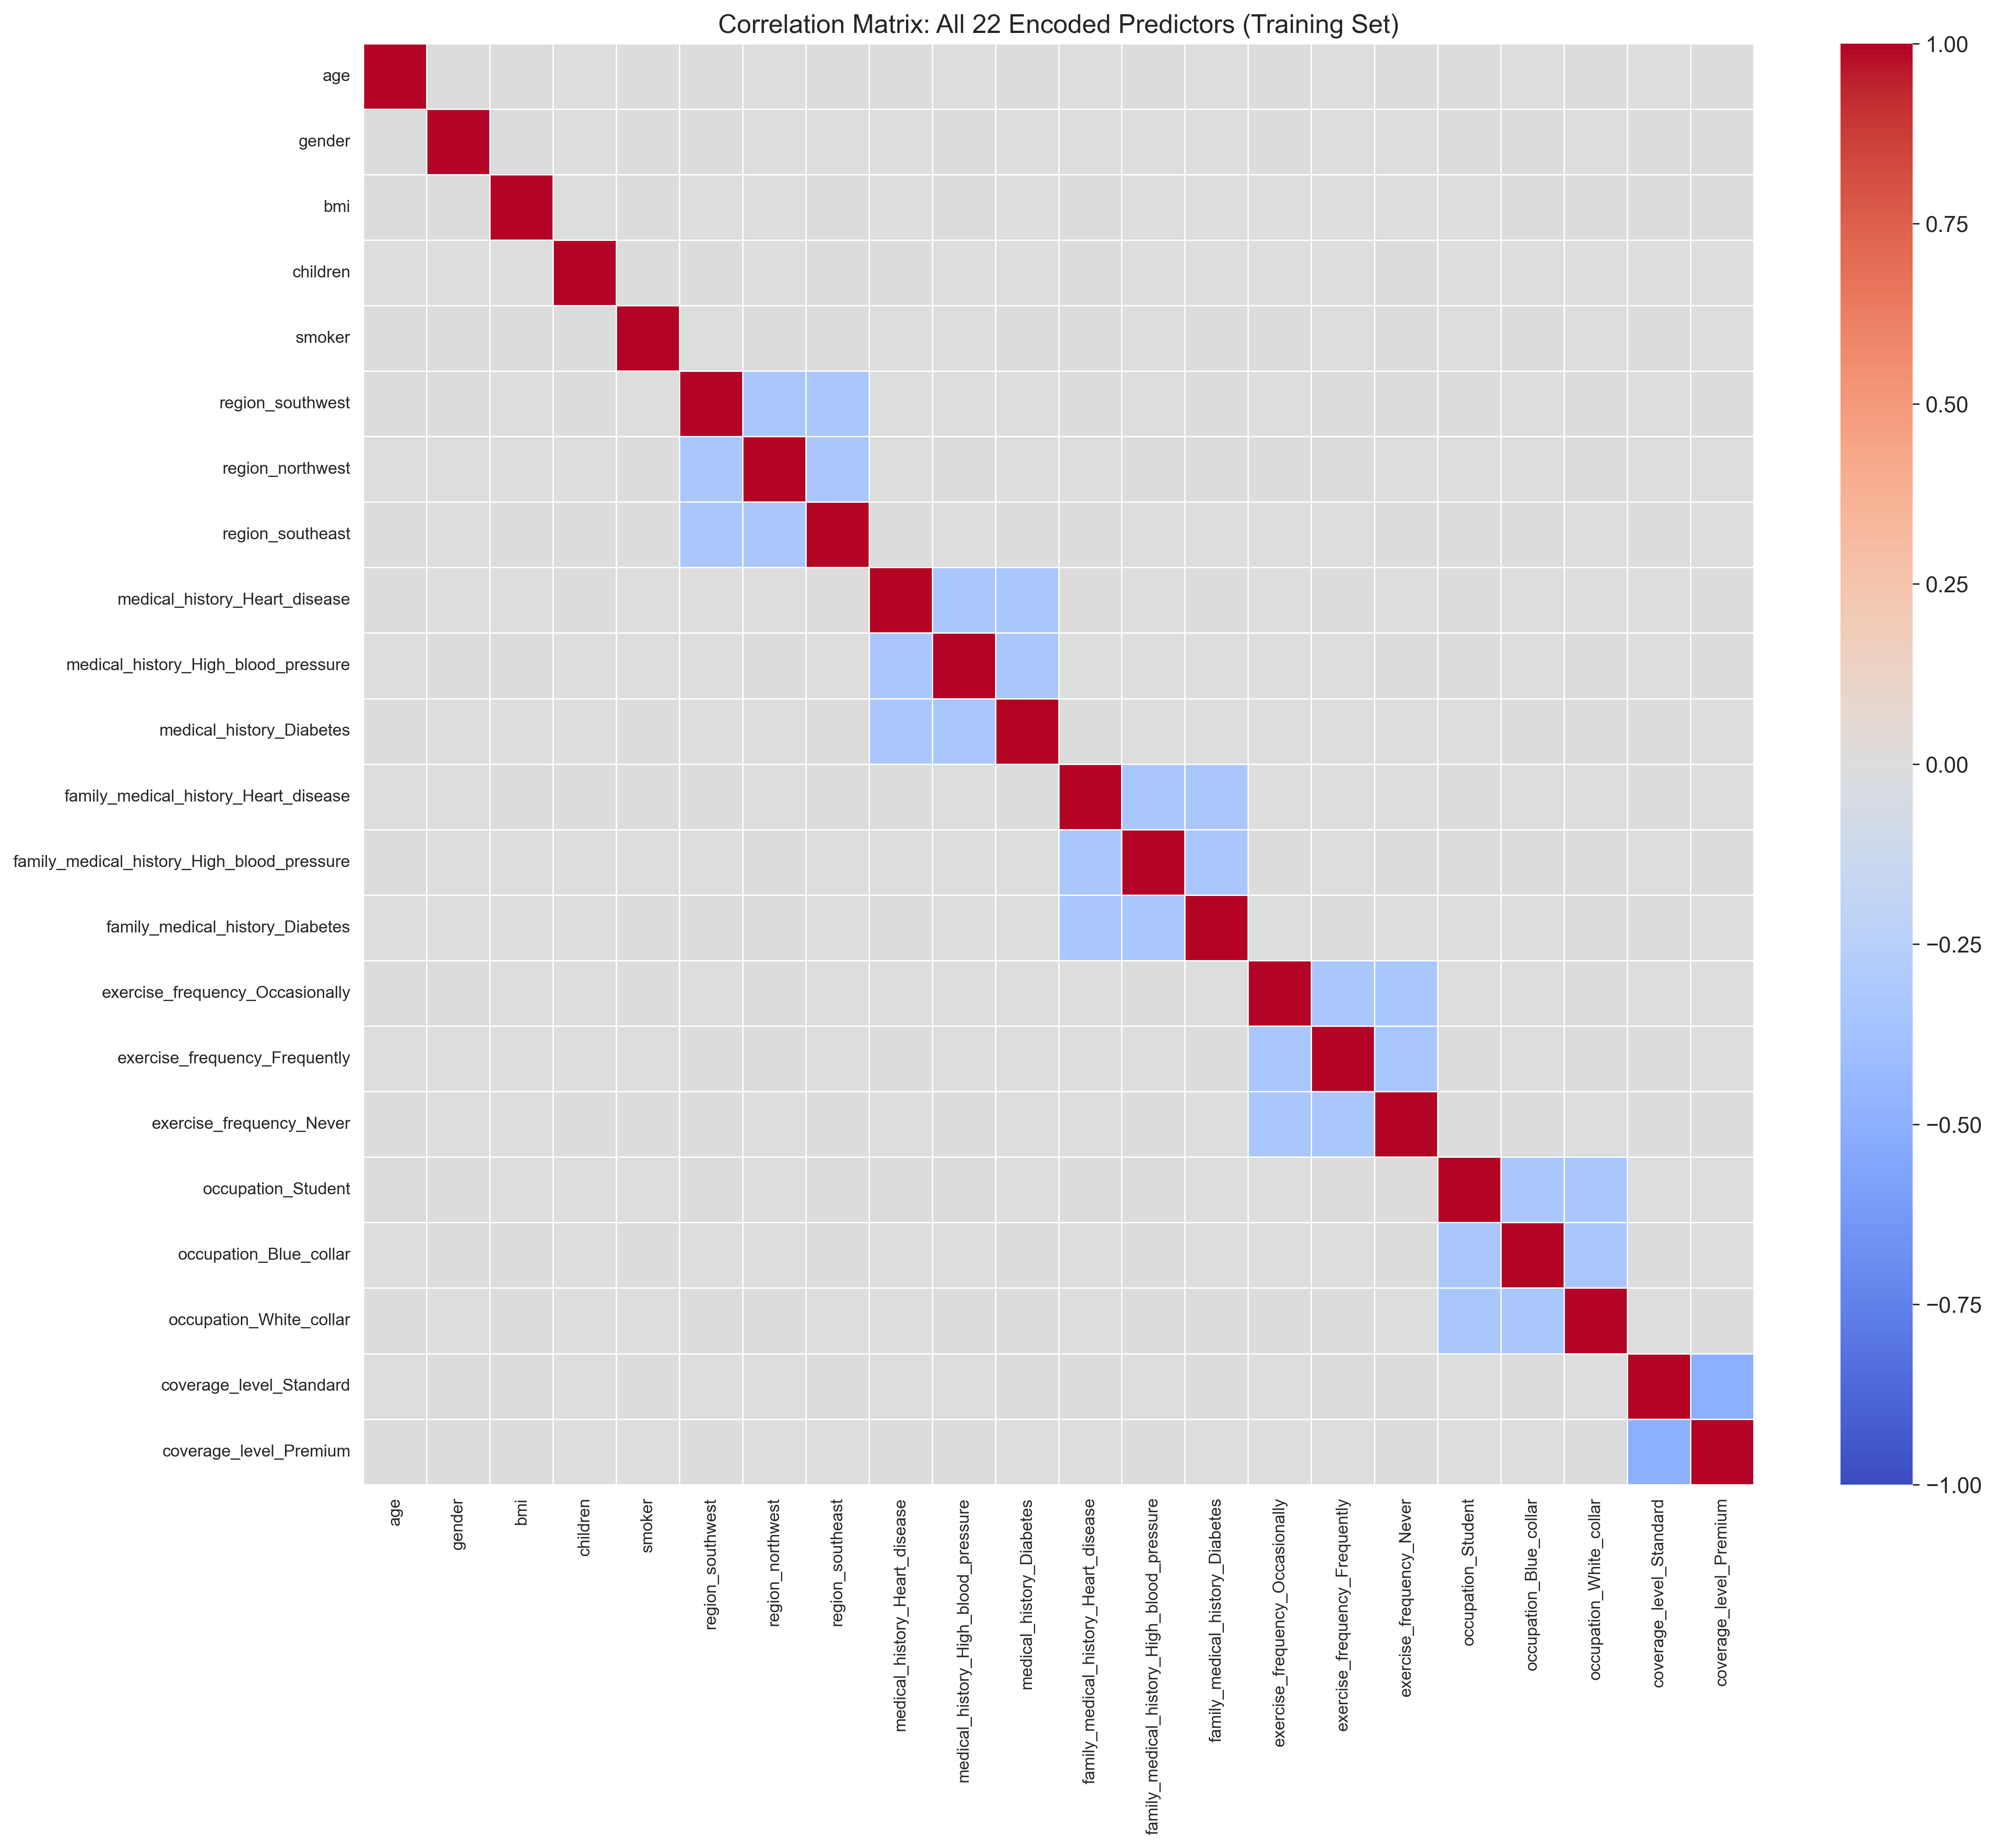
\includegraphics[width=\textwidth]{Thesis/Chapter 3/Figures/fig_full_encoded_correlation_heatmap.png}
    \caption{Full $22 \times 22$ Pearson correlation matrix of encoded predictors.}
    \label{fig:full_encoded_correlation_heatmap_ch3}
\end{subfigure}
\caption{Encoded predictor correlation analysis on the training partition.}
\label{fig:encoded_correlation_analysis_ch3}
\end{figure}

\noindent
Figure~\ref{fig:encoded_correlations_ch3} ranks all 22 encoded predictors
by their Pearson correlation with \texttt{charges}. The four strongest
positive associations are \texttt{smoker} ($r = 0.567$),\allowbreak{}
\texttt{coverage\_level\_\allowbreak{}Premium} ($r \approx 0.43$),\allowbreak{}
\texttt{medical\_history\_\allowbreak{}Heart\_disease} ($r \approx 0.39$) and
\texttt{family\_medical\_\allowbreak{}history\_\allowbreak{}Heart\_disease} ($r \approx 0.39$).
A second tier of moderate positive associations includes
\texttt{exercise\_frequency\_\allowbreak{}Frequently} ($r \approx 0.15$),\allowbreak{}
\texttt{occupation\_\allowbreak{}White\_collar} ($r \approx 0.12$),\allowbreak{}
\texttt{bmi}
($r \approx 0.10$), \texttt{children} ($r \approx 0.08$) and \texttt{age}
($r \approx 0.06$). On the negative side, the largest associations are
\texttt{medical\_history\_\allowbreak{}High\_blood\_\allowbreak{}pressure} ($r \approx -0.11$),\allowbreak{}
\texttt{family\_medical\_\allowbreak{}history\_\allowbreak{}High\_blood\_\allowbreak{}pressure}
($r \approx -0.10$),\allowbreak{}
\texttt{exercise\_frequency\_\allowbreak{}Never}
($r \approx -0.09$) and \texttt{gender} ($r \approx -0.08$). These
negative values reflect the reference-category encoding: for example,
a negative correlation for
\texttt{medical\_history\_\allowbreak{}High\_blood\_\allowbreak{}pressure} indicates lower charges
relative to the omitted reference category rather than a protective effect.
Figure~\ref{fig:full_encoded_correlation_heatmap_ch3} shows the full
inter-predictor correlation structure. The dominant feature is the block
of negative correlations within each dummy group: dummy indicators derived
from the same raw categorical variable are mechanically negatively
correlated because only one indicator can be active at a time. Outside
these within-group blocks, the off-diagonal correlations are uniformly
near zero (grey shading), confirming the absence of problematic
multicollinearity among predictors from different raw variables.

% ----------------------------
% 3.3.4 PARTITION CONSISTENCY
% ----------------------------

\subsubsection{Partition consistency}
Kernel density estimates of \texttt{charges} and of each numerical
predictor were overlaid for the training, validation, and test partitions;
the distributions are virtually indistinguishable.  Proportions of each
dummy variable were likewise compared, and no systematic shifts are
present.  The partitioning procedure therefore preserves the
distributional characteristics of the data.

% -------------------------------------------------
% 3.3.5 DECISIONS FROM THE EXPLORATORY DIAGNOSTICS
% -------------------------------------------------

\subsubsection{Decisions from the exploratory diagnostics}
Four implementation decisions follow directly from the EDA:

\begin{enumerate}
    \item Bounded numerical predictors are simulated under support
          restrictions that maintain their observed ranges.
    \item Categorical variables are simulated at the raw-category level
          and only afterwards encoded.
    \item The weak linear correlations among the numerical predictors,
          together with their uniform-like marginal shapes, motivate the
          product-marginal independence assumption adopted in the \gls{mc}
          design (Section~\ref{sec:mc_simulation_design}).
    \item The response is standardised during training and de-normalised
          for evaluation; no further transformation is needed.
\end{enumerate}

% ----------------------------------------
% 3.4 Network Specification and Training
% ----------------------------------------
\subsection{Network Specification and Training}
\label{sec:dnn_specification_training}

The predictive component is a \gls{dnn} for supervised
regression, following the formulation of equations~\eqref{eq:regression}
and~\eqref{eq:fitted_model}.  The network maps the model-ready input vector
$\mathbf{z}_i \in \mathbb{R}^{22}$ to a scalar prediction of the
standardised response,
\begin{equation}
    \widehat{\widetilde{y}}_i = f_{\widehat{\theta}}(\mathbf{z}_i),
    \label{eq:dnn_prediction_standardised_ch3}
\end{equation}
\equationlistentry{\Gls{dnn} prediction on standardised scale}
which is subsequently de-normalised to the original monetary scale via
equation~\eqref{eq:response_denormalisation_ch3}.

\subsubsection{Architecture}

The network adopts the contracting funnel topology

\begin{figure}[htbp]                                                                                                                                                                                               
  \centering                                                                                                                                                                                                       
  \begin{tikzpicture}[                                                                                                                                                                                               
      neuron/.style={circle, draw=black, fill=white, minimum size=10pt,                                                                                                                                            
                     inner sep=0pt, line width=0.4pt},                                                                                                                                                               
      dots/.style={minimum size=10pt, inner sep=0pt},                                                                                                                                                              
      layer label/.style={font=\footnotesize\bfseries, align=center},
      width label/.style={font=\scriptsize, text=black!70},
      connection/.style={-, draw=black!20, line width=0.2pt},
  ]

  % ── Horizontal positions ──
  \def\xIn{0}
  \def\xA{1.6}
  \def\xB{3.2}
  \def\xC{4.8}
  \def\xD{6.4}
  \def\xE{8.0}
  \def\xOut{9.6}

  % ── Vertical half-spans (centred at y = 0) ──
  \def\sIn{0.7}    % 22
  \def\sA{3.2}     % 256
  \def\sB{2.4}     % 128
  \def\sC{1.7}     % 64
  \def\sD{1.1}     % 32
  \def\sE{0.65}    % 16

  % === INPUT (22) ===
  \node[neuron] (i1) at (\xIn,  \sIn) {};
  \node[neuron] (i2) at (\xIn,  \sIn*0.33) {};
  \node[dots]        at (\xIn, -\sIn*0.2) {$\vdots$};
  \node[neuron] (i3) at (\xIn, -\sIn*0.55) {};
  \node[neuron] (i4) at (\xIn, -\sIn) {};
  \node[layer label, above=4pt of i1] {Input};
  \node[width label, below=4pt of i4] {22};

  % === HIDDEN 1 (256) ===
  \node[neuron] (a1) at (\xA,  \sA) {};
  \node[neuron] (a2) at (\xA,  \sA*0.65) {};
  \node[dots]        at (\xA,  \sA*0.35) {$\vdots$};
  \node[dots]        at (\xA,  0) {$\vdots$};
  \node[dots]        at (\xA, -\sA*0.35) {$\vdots$};
  \node[neuron] (a3) at (\xA, -\sA*0.65) {};
  \node[neuron] (a4) at (\xA, -\sA) {};
  \node[layer label, above=4pt of a1] {Hidden 1};
  \node[width label, below=4pt of a4] {256};

  % === HIDDEN 2 (128) ===
  \node[neuron] (b1) at (\xB,  \sB) {};
  \node[neuron] (b2) at (\xB,  \sB*0.55) {};
  \node[dots]        at (\xB,  0) {$\vdots$};
  \node[dots]        at (\xB, -\sB*0.3) {$\vdots$};
  \node[neuron] (b3) at (\xB, -\sB*0.65) {};
  \node[neuron] (b4) at (\xB, -\sB) {};
  \node[layer label, above=4pt of b1] {Hidden 2};
  \node[width label, below=4pt of b4] {128};

  % === HIDDEN 3 (64) ===
  \node[neuron] (c1) at (\xC,  \sC) {};
  \node[neuron] (c2) at (\xC,  \sC*0.4) {};
  \node[dots]        at (\xC, -\sC*0.15) {$\vdots$};
  \node[neuron] (c3) at (\xC, -\sC*0.55) {};
  \node[neuron] (c4) at (\xC, -\sC) {};
  \node[layer label, above=4pt of c1] {Hidden 3};
  \node[width label, below=4pt of c4] {64};

  % === HIDDEN 4 (32) ===
  \node[neuron] (d1) at (\xD,  \sD) {};
  \node[neuron] (d2) at (\xD,  \sD*0.33) {};
  \node[dots]        at (\xD, -\sD*0.2) {$\vdots$};
  \node[neuron] (d3) at (\xD, -\sD*0.55) {};
  \node[neuron] (d4) at (\xD, -\sD) {};
  \node[layer label, above=4pt of d1] {Hidden 4};
  \node[width label, below=4pt of d4] {32};

  % === HIDDEN 5 (16) ===
  \node[neuron] (e1) at (\xE,  \sE) {};
  \node[neuron] (e2) at (\xE,  \sE*0.33) {};
  \node[dots]        at (\xE, -\sE*0.2) {$\vdots$};
  \node[neuron] (e3) at (\xE, -\sE*0.55) {};
  \node[neuron] (e4) at (\xE, -\sE) {};
  \node[layer label, above=4pt of e1] {Hidden 5};
  \node[width label, below=4pt of e4] {16};

  % === OUTPUT (1) ===
  \node[neuron] (o1) at (\xOut, 0) {};
  \node[layer label, above=4pt of o1] {Output};
  \node[width label, below=4pt of o1] {1};

  % === CONNECTIONS ===
  \foreach \src in {i1,i2,i3,i4}{
      \foreach \dst in {a1,a2,a3,a4}{ \draw[connection] (\src) -- (\dst); }}
  \foreach \src in {a1,a2,a3,a4}{
      \foreach \dst in {b1,b2,b3,b4}{ \draw[connection] (\src) -- (\dst); }}
  \foreach \src in {b1,b2,b3,b4}{
      \foreach \dst in {c1,c2,c3,c4}{ \draw[connection] (\src) -- (\dst); }}
  \foreach \src in {c1,c2,c3,c4}{
      \foreach \dst in {d1,d2,d3,d4}{ \draw[connection] (\src) -- (\dst); }}
  \foreach \src in {d1,d2,d3,d4}{
      \foreach \dst in {e1,e2,e3,e4}{ \draw[connection] (\src) -- (\dst); }}
  \foreach \src in {e1,e2,e3,e4}{
      \draw[connection] (\src) -- (o1); }

  \end{tikzpicture}
  \caption{Funnel architecture of the \gls{dnn}.}
  \label{fig:dnn_architecture_ch3}
  \end{figure}

with the layer-wise recursion given by
equation~\eqref{eq:pre_activation}.  All hidden layers use the
\gls{celu} activation function
(equation~\eqref{eq:celu}).  \gls{celu} was selected from among the
candidate activations reviewed in
Section~\ref{sec:activation_functions} because it combines the
computational efficiency of a rectifier with continuous
differentiability across its entire domain, avoiding the dead-unit
problem associated with \gls{relu} while maintaining a linear positive
branch that preserves gradient flow in deep architectures.  The output
layer uses an identity mapping, as required for continuous regression.  The full five-hidden-layer depth,
including the final 16-unit layer, is retained; its adequacy is assessed
through the validation diagnostics of
Section~\ref{sec:model_validation_diagnostics}.

The network is constructed without bias vectors.  This is a genuine
restriction rather than a costless simplification: because the \gls{celu}
activation satisfies $\sigma(0)=0$, a bias-free network necessarily maps
the origin to zero, so the fitted function is pinned to zero at the
standardised data centroid and cannot represent arbitrary additive shifts
(the corresponding universal-approximation caveat is discussed in
Chapter~\ref{sec:literature_review}).  After standardisation, however, the
data centroid maps near the origin, where the response surface lies well
within the support of the data, and the adequacy of the bias-free
restriction is assessed empirically through the predictive diagnostics of
Section~\ref{sec:model_validation_diagnostics} rather than guaranteed
theoretically.  The total number of trainable parameters is
\begin{align}
    N_{\mathrm{par}}
    &= (22)(256) + (256)(128) + (128)(64) + (64)(32) + (32)(16) + (16)(1) \notag \\
    &= 49\,168.
    \label{eq:dnn_parameter_count_ch3}
\end{align}
\equationlistentry{\Gls{dnn} total trainable parameter count}

\subsubsection{Forward and Backward Propagation}
\label{sec:propagation_mechanics}

The operation of the contracting funnel specified in figure
\ref{fig:dnn_architecture_ch3} can be described compactly by the
forward- and backward-pass equations that underpin all gradient-based
training.  For a single input vector $\mathbf{x}$ (with
$\mathbf{a}^{(0)} = \mathbf{x}$), the forward computation of layer $l$ is
\begin{align}
    \mathbf{z}^{(l)} &= \bigl(W^{(l)}\bigr)^{\!\top} \mathbf{a}^{(l-1)}
                      + \mathbf{b}^{(l)},
                      \qquad
                      W^{(l)} \in \mathbb{R}^{d_{l-1}\times d_{l}},\;
                      \mathbf{b}^{(l)} \in \mathbb{R}^{d_{l}},
    \label{eq:forward_affine} \\
    \mathbf{a}^{(l)} &= \sigma_l\!\bigl(\mathbf{z}^{(l)}\bigr),
    \label{eq:forward_activation}
\end{align}
where $d_{l-1}$ and $d_{l}$ are the widths of the adjacent layers.
Because the input and response are standardised and the architecture omits
bias vectors (Section~\ref{sec:dnn_specification_training}), the bias term
is not used; the forward pass simplifies to
equation~\eqref{eq:bias_free_recursion}.

The network is trained by minimising the \gls{mse} loss
$\mathcal{L} = \frac{1}{2}(y - \hat{y})^{2}$.  Defining the gradient of the
loss with respect to the output pre-activation as
\begin{equation}
    \delta^{(L)} \equiv \frac{\partial \mathcal{L}}{\partial \mathbf{z}^{(L)}}
    = \hat{y} - y,
    \label{eq:output_delta}
\end{equation}
this error signal is propagated backward through the hidden layers.  For
layer $l = L-1, L-2, \dots, 1$, the recursion is
\begin{equation}
    \delta^{(l)}
    = \frac{\partial \mathcal{L}}{\partial \mathbf{z}^{(l)}}
    = \bigl(W^{(l+1)}\bigr)^{\!\top} \delta^{(l+1)}
      \odot \sigma_{l}'\!\bigl(\mathbf{z}^{(l)}\bigr),
    \label{eq:backprop_delta}
\end{equation}
where $\odot$ denotes element-wise multiplication and $\sigma_{l}'$ is the
derivative of the activation function.  For the \gls{celu} activation
employed in every hidden layer (equation~\eqref{eq:celu}), the derivative is
smooth and non-zero for all inputs, ensuring stable gradient flow.

The gradient of the loss with respect to the weight matrix of layer $l$ is
\begin{equation}
    \frac{\partial \mathcal{L}}{\partial W^{(l)}}
    = \mathbf{a}^{(l-1)} \bigl(\delta^{(l)}\bigr)^{\!\top}.
    \label{eq:weight_gradient}
\end{equation}
Because bias vectors are omitted, no bias-update term appears.  The weight
matrices are then updated by the \gls{nadam} optimiser
(Section~\ref{sec:training_configuration}), which combines Nesterov-accelerated momentum with adaptive learning rates.

These equations are standard in the deep learning literature
\citep{goodfellow2016deep} and are reproduced here for completeness; they
make the training procedure, including the bias-free simplification,
explicit.  In practice, all gradients are computed automatically by
the deep learning framework (PyTorch) through reverse-mode automatic
differentiation, so the closed-form expressions are never coded directly.
Their inclusion ensures that the reader can relate the chosen architecture,
loss function, and activation to the mechanics of gradient-based
optimisation.


\subsubsection{Training configuration}
\label{sec:training_configuration}

The network is trained by minimising the \gls{mse} on the
standardised response scale (equation~\eqref{eq:mse_loss}).  Weights are
updated with the \gls{nadam} optimiser \citep{dozat2016incorporating}, described
in Section~\ref{sec:loss_optimisation}.  Validation performance is
evaluated every $v = 5$ epochs.  For a fixed validation set, minimising
the validation \gls{mse} is equivalent to maximising the validation \gls{r2}; the
dot-product \gls{r2} is therefore used as the operational model-selection
criterion.  The selected epoch is
\begin{equation}
    e^{*} = \arg\max_{e \in \mathcal{E}_{\mathrm{val}}} R^2_{\mathrm{val}}(e),
    \qquad
    \mathcal{E}_{\mathrm{val}} = \{v, 2v, 3v, \dots\} \cap \{1, \dots, E_{\max}\}.
    \label{eq:validation_r2_epoch_selection_ch3}
\end{equation}
\equationlistentry{Validation $R^2$ epoch selection criterion}
Training stops early if the validation \gls{r2} does not improve for $P = 10$
consecutive validation checks \citep{prechelt2012early}; the retained
model is the checkpoint with the highest validation \gls{r2} observed.  The test set is reserved
exclusively for final out-of-sample evaluation.

On the original monetary scale, the standard
$R^2 = 1 - \mathrm{SS}_{\mathrm{res}} / \mathrm{SS}_{\mathrm{tot}}$
(equation~\eqref{eq:r_squared}) is reported alongside the \gls{mae} and
\gls{rmse}.

Table~\ref{tab:dnn_architecture_training_ch3} summarises the complete
architecture and training configuration.

\begin{table}[H]
\centering
\small
\renewcommand{\arraystretch}{1.15}
\begin{tabular}{p{0.34\textwidth}p{0.56\textwidth}}
\toprule
\textbf{Component} & \textbf{Specification} \\
\midrule
Input dimension & $p = 22$ encoded predictor variables \\
Hidden layer widths & $256, 128, 64, 32, 16$ \\
Output dimension & One scalar regression output \\
Architecture type & Fully connected \gls{dnn} \\
Network shape & Contracting representation from 256 to 16 hidden units \\
Bias vectors & Omitted \\
Hidden activation & \gls{celu} (equation~\eqref{eq:celu}) \\
Output activation & Identity mapping \\
Training response & Standardised \texttt{charges} \\
Prediction scale & De-normalised to the original monetary scale \\
Training objective & \Gls{mse} on the standardised response scale \\
Secondary evaluation metrics & \gls{mae}, \gls{rmse} and \gls{r2} on the original response scale \\
Optimiser & \gls{nadam} \citep{dozat2016incorporating} \\
Momentum parameters & $(\beta_1,\beta_2)$ selected by validation comparison from $\{(0.90,0.999),\ (0.95,0.999),\ (0.99,0.999)\}$ \\
Learning rate & Selected by validation comparison from $\{0.01, 0.001, 0.0005, 0.0001\}$ \\
Batch size & Selected by validation comparison from $\{64, 128, 256, 512\}$ \\
Maximum epochs & $E_{\max} = 200$ \\
Validation frequency & Every $v = 5$ epochs \\
Model-selection criterion & Dot-product validation \gls{r2} \\
Early stopping & Patience $P = 10$ validation checks without \gls{r2} improvement \\
Explicit regularisation & Not used \\
Dropout & Not used \\
Random seed & $s = 42$, fixed for reproducibility \\
Trainable parameters & $49\,168$ weights \\
\bottomrule
\end{tabular}
\caption{\Gls{dnn} architecture and training configuration.}
\label{tab:dnn_architecture_training_ch3}
\end{table}

\subsubsection{Hyperparameter comparison}

The main training hyperparameters that materially affect the fitted
prediction surface are compared sequentially:

\begin{enumerate}
    \item \textbf{Hidden activation:}  \gls{celu}, \gls{gelu} and Tanh are evaluated
          with learning rate $0.001$, batch size $256$, and \gls{adam} held fixed.
    \item \textbf{Learning rate:}  Values $\{0.01, 0.001, 0.0005, 0.0001\}$
          are tested with the best activation carried forward.
    \item \textbf{Batch size:}  Sizes $\{64, 128, 256, 512\}$ are tested
          with the best activation and learning rate.
    \item \textbf{Optimiser:}  \gls{adam} and \gls{nadam} are compared with all previous
          best choices carried forward.
    \item \textbf{Momentum parameters:} $(\beta_1,\beta_2)$.  Since \gls{nadam} is
          selected in the previous step, its Nesterov-accelerated momentum
          parameters are compared over
          $\{(0.90,0.999),\linebreak[1] (0.95,0.999),\linebreak[1] (0.99,0.999)\}$.  The first
          coefficient $\beta_1$ controls the decay of the gradient mean
          estimate; the second, $\beta_2$, controls the decay of the
          uncentred variance estimate \citep{dozat2016incorporating}.
\end{enumerate}

At each stage the best choice is carried forward and all other factors are
held constant.  Explicit $\mathcal{L}_1$, $\mathcal{L}_2$, and dropout
\citep{srivastava2014dropout} regularisation are not
included; the adequacy of this design is assessed through validation
curves, out-of-sample error metrics, and structural diagnostics\footnote{In this context, $\mathcal{L}_1$ and $\mathcal{L}_2$
regularisation refer to adding penalty terms to the training objective. If
\(\mathcal{L}_{0}(\theta)\) denotes the original training loss and
\(\theta=(\theta_1,\ldots,\theta_d)\) denotes the vector of trainable
parameters, then $\mathcal{L}_1$ regularisation uses
\[
    \mathcal{L}_{1}(\theta)
    =
    \mathcal{L}_{0}(\theta)
    +
    \lambda
    \sum_{j=1}^{d}
    |\theta_j|,
\]
whereas $\mathcal{L}_2$ regularisation uses
\[
    \mathcal{L}_{2}(\theta)
    =
    \mathcal{L}_{0}(\theta)
    +
    \lambda
    \sum_{j=1}^{d}
    \theta_j^2.
\]
Here, \(\lambda \geq 0\) controls the strength of the penalty. The $\mathcal{L}_1$
penalty encourages sparse parameter estimates, while the $\mathcal{L}_2$ penalty
shrinks parameters towards zero without necessarily setting them exactly equal
to zero.}.

The training procedure consists of: (1)~random weight initialisation
using Kaiming uniform initialisation \citep{he2015delving}, which
scales the initial weights according to the fan-in of each layer so
that activations neither vanish nor explode during the early forward
passes, a property that is particularly important in deeper
architectures such as the five-hidden-layer network used here;
(2)~mini-batch gradient descent with the \gls{nadam} optimiser;
(3)~validation evaluation every 5 epochs using the dot-product \gls{r2};
(4)~early stopping when the validation \gls{r2} has not improved for 10
consecutive checks; (5)~selection of the checkpoint with the highest
validation \gls{r2}; and (6)~final test-set evaluation on the original
monetary scale using \gls{r2}, \gls{rmse} and \gls{mae}.  The complete
pseudocode is presented in
Algorithm~\ref{tab:dnn_training_algorithm_annex}
(\ref{annexure:dnn_algorithm_detailed}).

\subsubsection{Benchmark GLM}
\label{sec:glm_benchmark_methods}

A classical actuarial benchmark is provided by a \gls{glm}
with a gamma distribution and logarithmic link function
\citep{dobson2008introduction, mccullagh1989generalized}.  For a policyholder with
model-ready input vector $\mathbf{z}_i \in \mathbb{R}^{22}$ (the same encoded
predictors used by the \gls{dnn}), the \gls{glm} assumes
\begin{equation}
    Y_i \sim \text{Gamma}(\mu_i, \phi),
    \qquad
    \log(\mu_i) = \beta_0 + \sum_{j=1}^{22} \beta_j z_{ij},
    \label{eq:glm_specification}
\end{equation}
\equationlistentry{\Gls{glm} specification with gamma distribution and log link}
where $\mu_i = \mathbb{E}[Y_i \mid \mathbf{z}_i]$ and $\phi$ is the
dispersion parameter.  The distributional and link-function rationale
for this specification was set out in
Section~\ref{sec:classical_actuarial}; under the log link the predicted
mean $\mu_i = \exp(\beta_0 + \sum_j \beta_j z_{ij})$ is always positive.

The model includes no interaction terms or non-linear transformations.  It
is fitted to the training partition by maximum likelihood estimation.  The
log-likelihood for the gamma \gls{glm} is
\begin{equation}
    \ell(\boldsymbol{\beta}, \phi)
    =
    \sum_{i=1}^{n}
    \left[
        \frac{1}{\phi}
        \left(
            -\frac{y_i}{\mu_i} - \log \mu_i
        \right)
        +
        \left(\frac{1}{\phi} - 1\right) \log y_i
        -
        \log \Gamma\!\left(\frac{1}{\phi}\right)
        -
        \frac{1}{\phi}\log \phi
    \right],
    \label{eq:glm_loglikelihood}
\end{equation}
\equationlistentry{Gamma \gls{glm} log-likelihood}
where $\mu_i = \exp(\mathbf{z}_i^{\top}\boldsymbol{\beta})$ and
$\boldsymbol{\beta} = (\beta_0, \beta_1, \ldots, \beta_{22})^{\top}$.
The parameter vector $\boldsymbol{\beta}$ is estimated by \gls{irls}, which solves the score equations
\begin{equation}
    \sum_{i=1}^{n}
    \frac{(y_i - \mu_i)}{\mathrm{Var}(Y_i)}
    \,
    \frac{\partial \mu_i}{\partial \eta_i}
    \,
    z_{ij}
    = 0,
    \qquad j = 0, 1, \ldots, 22,
    \label{eq:glm_score}
\end{equation}
\equationlistentry{\Gls{glm} score equations}
where $\eta_i = \log(\mu_i)$ is the linear predictor and
$\mathrm{Var}(Y_i) = \phi\,\mu_i^{2}$ under the gamma family.  Each \gls{irls}
iteration computes a weighted least squares regression of an adjusted
dependent variable on the design matrix, with weights inversely
proportional to the variance function evaluated at the current fitted
values \citep{dobson2008introduction}.

Algorithm~\ref{tab:glm_algorithm_annex} formalises the fitting procedure.

The \gls{glm} is fitted via \gls{irls},
which computes working weights and adjusted dependent variables at each
iteration until convergence.  The dispersion parameter
$\widehat{\phi}$ is estimated from the Pearson residuals, and
predictions are obtained on the original monetary scale by applying the
inverse link $\widehat{y}_i = \exp(\mathbf{z}_i^{\top}
\widehat{\boldsymbol{\beta}})$.  The complete \gls{irls} algorithm is
presented in Algorithm~\ref{tab:glm_algorithm_annex}
(\ref{annexure:glm_algorithm}).

No hyperparameter tuning is applied to the \gls{glm}; its role as a benchmark
was motivated in Section~\ref{sec:statistical_learning_supervised_regression}.

\subsubsection{Tree-Based Benchmarks}
\label{sec:tree_benchmarks_methods}

Two tree-based ensemble methods are included alongside the \gls{glm} to
provide a more comprehensive model-class comparison.  Both models use the
same 22 encoded features and the same approximately $52/24/24$ partition
(Section~\ref{sec:feature_encoding_input_standardisation}) as the
\gls{dnn} and \gls{glm}.

% ----- \Gls{rf} -----

\subsubsection{RF Benchmark}
A \gls{rf} regressor \citep{breiman2001random} is fitted with 500 trees,
maximum depth unrestricted, minimum samples per leaf of 5, and
\texttt{random\_state=42}.  \gls{rf} aggregates predictions across
decorrelated decision trees, reducing variance through bootstrap
aggregation (bagging) while maintaining low bias.

The \gls{rf} constructs an ensemble of $B$ regression trees, each grown on
a bootstrap sample of the training data.  At every candidate split the
algorithm considers only a random subset of $m$ out of $p$ predictors,
thereby decorrelating the individual trees and reducing the variance of the
averaged prediction.  For a regression tree $T_b$ grown on bootstrap
sample $\mathcal{D}_b^{*}$, the prediction for input $\mathbf{z}$ is
$\hat{y}_b(\mathbf{z}) = T_b(\mathbf{z})$.  The \gls{rf} prediction is
the average across all $B$ trees:
\begin{equation}
    \hat{f}_{\mathrm{RF}}(\mathbf{z})
    =
    \frac{1}{B}
    \sum_{b=1}^{B}
    T_b(\mathbf{z}).
    \label{eq:rf_prediction}
\end{equation}
\equationlistentry{\Gls{rf} ensemble prediction}

Each tree $T_b$ is grown by recursively partitioning the feature space.
At each internal node, the algorithm selects a random subset of
$m = \lfloor p/3 \rfloor$ predictors (the default for regression) and
chooses the split variable $j^{*}$ and split point $s^{*}$ that minimise
the weighted sum of squared residuals in the resulting child nodes:
\begin{equation}
    (j^{*}, s^{*})
    =
    \arg\min_{j \in \mathcal{S},\; s}
    \Biggl[
        \sum_{i:\, z_{ij} \le s} (y_i - \bar{y}_{L})^{2}
        +
        \sum_{i:\, z_{ij} > s} (y_i - \bar{y}_{R})^{2}
    \Biggr],
    \label{eq:rf_split_criterion}
\end{equation}
\equationlistentry{\Gls{rf} split criterion}
where $\mathcal{S} \subset \{1,\dots,p\}$ with $|\mathcal{S}| = m$ is the
randomly selected predictor subset, and $\bar{y}_{L}$ and $\bar{y}_{R}$
denote the sample means in the left and right child nodes respectively.
Trees are grown until each terminal node contains at most 5 observations.

The variance reduction mechanism of the \gls{rf} can be understood
through the decomposition of the variance of the ensemble average.  If
individual tree predictions have variance $\sigma^{2}$ and pairwise
correlation $\rho$, then
\begin{equation}
    \mathrm{Var}\bigl(\hat{f}_{\mathrm{RF}}\bigr)
    =
    \rho\,\sigma^{2}
    +
    \frac{1 - \rho}{B}\,\sigma^{2}.
    \label{eq:rf_variance_reduction}
\end{equation}
\equationlistentry{\Gls{rf} variance reduction}
As $B$ increases, the second term vanishes, and the ensemble variance is
governed by $\rho\,\sigma^{2}$.  By restricting splits to a random
predictor subset, the \gls{rf} reduces $\rho$ below the value obtained by
standard bagging (which uses all $p$ predictors at every split), yielding
a lower ensemble variance \citep{hastie2009elements}.

The complete training procedure is presented in
Algorithm~\ref{tab:rf_algorithm_annex}
(\ref{annexure:rf_algorithm}), and
Table~\ref{tab:rf_hyperparameters_ch3} summarises the \gls{rf}
configuration.

\begin{table}[H]
\centering
\small
\renewcommand{\arraystretch}{1.15}
\begin{tabular}{p{0.34\textwidth}p{0.56\textwidth}}
\toprule
\textbf{Component} & \textbf{Specification} \\
\midrule
Number of trees ($B$) & 500 \\
Candidate predictors per split ($m$) & $\lfloor p/3 \rfloor = 7$ \\
Maximum depth & Unrestricted \\
Minimum samples per leaf & 5 \\
Bootstrap sampling & With replacement, sample size $= n_{\mathrm{train}}$ \\
Split criterion & \Gls{mse} (equation~\eqref{eq:rf_split_criterion}) \\
Hyperparameter tuning & Not applied (default values) \\
Random seed & 42 \\
Implementation & \texttt{scikit-learn} \texttt{Random\allowbreak{}Forest\allowbreak{}Regressor} \\
\bottomrule
\end{tabular}
\caption{\Gls{rf} configuration.}
\label{tab:rf_hyperparameters_ch3}
\end{table}

% ----- XGBoost -----

\subsubsection{XGBoost Benchmark}
A gradient-boosted tree regressor is fitted using the \gls{xgboost}
implementation \citep{chen2016xgboost} with 1\,000 boosting rounds, a
learning rate of 0.05, maximum depth of 8, and early stopping on the
validation set with a patience of 50 rounds.  \gls{xgboost} constructs an
additive ensemble of shallow trees via gradient boosting, using
approximate histogram-based splitting for computational efficiency.

Gradient boosting builds an additive model in a stage-wise fashion.  The
ensemble prediction after $M$ boosting rounds is
\begin{equation}
    \hat{f}_{M}(\mathbf{z})
    =
    \sum_{m=0}^{M}
    \eta \, h_m(\mathbf{z}),
    \label{eq:xgb_additive_model}
\end{equation}
\equationlistentry{\Gls{xgboost} additive ensemble model}
where $h_0(\mathbf{z}) = \bar{y}$ is the initial constant prediction
(the training-set mean), $h_m$ is the regression tree fitted at round $m$,
and $\eta \in (0,1]$ is the learning rate (shrinkage parameter) that
scales each tree's contribution.

At each boosting round $m$, \gls{xgboost} fits a new tree $h_m$ to
minimise a regularised objective.  For the squared-error loss used in
regression, the objective at round $m$ is
\begin{equation}
    \mathcal{O}^{(m)}
    =
    \sum_{i=1}^{n}
    \ell\!\bigl(y_i,\, \hat{f}_{m-1}(\mathbf{z}_i) + h_m(\mathbf{z}_i)\bigr)
    +
    \Omega(h_m),
    \label{eq:xgb_objective}
\end{equation}
\equationlistentry{\Gls{xgboost} regularised objective}
where $\ell(y, \hat{y}) = \tfrac{1}{2}(y - \hat{y})^{2}$ is the
squared-error loss and $\Omega(h_m)$ is a regularisation penalty on the
complexity of tree $h_m$.  The regularisation term is defined as
\begin{equation}
    \Omega(h)
    =
    \gamma \, J
    +
    \tfrac{1}{2}\,\lambda
    \sum_{j=1}^{J}
    w_j^{2},
    \label{eq:xgb_regularisation}
\end{equation}
\equationlistentry{\Gls{xgboost} tree complexity penalty}
where $J$ is the number of terminal nodes (leaves), $w_j$ is the
predicted value in leaf $j$, $\gamma \ge 0$ penalises additional leaves,
and $\lambda \ge 0$ applies $\mathcal{L}_2$ shrinkage to the leaf weights.

The key computational innovation of \gls{xgboost} is the use of a
second-order Taylor expansion of the loss around the current prediction
$\hat{f}_{m-1}(\mathbf{z}_i)$.  Define the first- and second-order
gradient statistics for observation $i$:
\begin{equation}
    g_i
    =
    \frac{\partial\, \ell(y_i,\, \hat{y})}{\partial\, \hat{y}}
    \bigg|_{\hat{y} = \hat{f}_{m-1}(\mathbf{z}_i)},
    \qquad
    h_i
    =
    \frac{\partial^{2}\, \ell(y_i,\, \hat{y})}{\partial\, \hat{y}^{2}}
    \bigg|_{\hat{y} = \hat{f}_{m-1}(\mathbf{z}_i)}.
    \label{eq:xgb_gradient_hessian}
\end{equation}
\equationlistentry{\Gls{xgboost} gradient and Hessian statistics}
For the squared-error loss, $g_i = \hat{f}_{m-1}(\mathbf{z}_i) - y_i$
(the negative residual) and $h_i = 1$.  With these gradient statistics,
the approximate objective simplifies to
\begin{equation}
    \tilde{\mathcal{O}}^{(m)}
    =
    \sum_{j=1}^{J}
    \Biggl[
        G_j \, w_j
        +
        \frac{1}{2}(H_j + \lambda)\, w_j^{2}
    \Biggr]
    +
    \gamma \, J,
    \label{eq:xgb_approx_objective}
\end{equation}
\equationlistentry{\Gls{xgboost} second-order approximate objective}
where $G_j = \sum_{i \in I_j} g_i$ and $H_j = \sum_{i \in I_j} h_i$ are
the sums of gradient and Hessian statistics over the observations
$I_j$ assigned to leaf $j$.  The optimal leaf weight and the
corresponding optimal objective value are
\begin{equation}
    w_j^{*}
    =
    -\frac{G_j}{H_j + \lambda},
    \qquad
    \tilde{\mathcal{O}}^{*}
    =
    -\frac{1}{2}
    \sum_{j=1}^{J}
    \frac{G_j^{2}}{H_j + \lambda}
    +
    \gamma \, J.
    \label{eq:xgb_optimal_leaf}
\end{equation}
\equationlistentry{\Gls{xgboost} optimal leaf weight and objective}

To evaluate a candidate split that partitions observations in a node into
left ($I_L$) and right ($I_R$) child nodes, \gls{xgboost} computes the
gain:
\begin{equation}
    \mathrm{Gain}
    =
    \frac{1}{2}
    \left[
        \frac{G_L^{2}}{H_L + \lambda}
        +
        \frac{G_R^{2}}{H_R + \lambda}
        -
        \frac{(G_L + G_R)^{2}}{H_L + H_R + \lambda}
    \right]
    -
    \gamma,
    \label{eq:xgb_split_gain}
\end{equation}
\equationlistentry{\Gls{xgboost} split gain criterion}
where $G_L = \sum_{i \in I_L} g_i$, $G_R = \sum_{i \in I_R} g_i$,
$H_L = \sum_{i \in I_L} h_i$, and $H_R = \sum_{i \in I_R} h_i$.  A
split is made only if $\mathrm{Gain} > 0$; the regularisation parameter
$\gamma$ acts as a minimum-gain threshold that prunes unprofitable splits
\citep{chen2016xgboost}.

The complete training procedure is presented in
Algorithm~\ref{tab:xgb_algorithm_annex}
(\ref{annexure:xgb_algorithm}), and
Table~\ref{tab:xgb_hyperparameters_ch3} summarises the \gls{xgboost}
configuration.

\begin{table}[H]
\centering
\small
\renewcommand{\arraystretch}{1.15}
\begin{tabular}{p{0.34\textwidth}p{0.56\textwidth}}
\toprule
\textbf{Component} & \textbf{Specification} \\
\midrule
Maximum boosting rounds ($M$) & 1\,000 \\
Learning rate ($\eta$) & 0.05 \\
Maximum tree depth ($d_{\max}$) & 8 \\
Booster & \texttt{gbtree} (tree-based) \\
Objective & \texttt{reg:squarederror} \\
Split evaluation & Approximate histogram-based \\
$\mathcal{L}_2$ regularisation ($\lambda$) & Default (1.0) \\
Minimum split gain ($\gamma$) & Default (0.0) \\
Early stopping patience & 50 rounds on validation loss \\
Hyperparameter tuning & Not applied (default values) \\
Random seed & 42 \\
Implementation & \texttt{xgboost} \texttt{XGBRegressor} \\
\bottomrule
\end{tabular}
\caption{\Gls{xgboost} configuration.}
\label{tab:xgb_hyperparameters_ch3}
\end{table}

In the primary comparison, hyperparameters for both tree-based models are
set to commonly recommended defaults rather than tuned via
cross-validation, paralleling the no-tuning treatment of the \gls{glm};
this isolates model-class differences from tuning effort.  As a
complementary analysis, both tree-based models are subsequently re-fitted
with tuned hyperparameters selected by randomised search with five-fold
cross-validation on the training partition, quantifying how much of any
remaining performance gap is attributable to tuning rather than to the
model class itself (results in Section~\ref{sec:tuned_benchmarks}).  All
models are evaluated using $R^2$, \gls{rmse} and \gls{mae} on the
original monetary scale across all three partitions.

% =============================================================
\subsection{Predictive and Structural Diagnostics}
\label{sec:model_validation_diagnostics}
\label{sec:model_evaluation_metrics}
\label{sec:fitted_model_diagnostic_plots}

The predictive and structural diagnostics described below serve a single
purpose: to verify that the fitted \gls{dnn} is sufficiently stable and
well-behaved to act as the prediction surface in the subsequent \gls{mc}
and Shapley-value analyses.

All predictive performance metrics are computed on the original monetary
scale after de-normalising the fitted predictions.  The metrics are the
\gls{mae}, \gls{rmse} and $R^2$ defined in
equations~\eqref{eq:mae},~\eqref{eq:rmse} and~\eqref{eq:r_squared}.  For
observation $i$ the fitted prediction is denoted $\widehat{y}_i$ and
the residual is
\begin{equation}
    r_i = y_i - \widehat{y}_i .
    \label{eq:residual_definition_ch3}
\end{equation}
\equationlistentry{Residual definition}
Residuals are computed separately for the training, validation and test
partitions.

\subsubsection{Predictive error assessment}

Predictive error is assessed by comparing observed charges with fitted
predictions on the original response scale.  The training partition is used
to evaluate in-sample fit, the validation partition to guide model-selection
decisions, and the test partition to provide a final out-of-sample
evaluation.  The three scalar metrics are interpreted jointly: a suitable
model should exhibit consistent performance across the validation and test
partitions, without a large deterioration relative to the training
partition.

\begin{figure}[H]
\centering
\begin{subfigure}[b]{\textwidth}
    \centering
    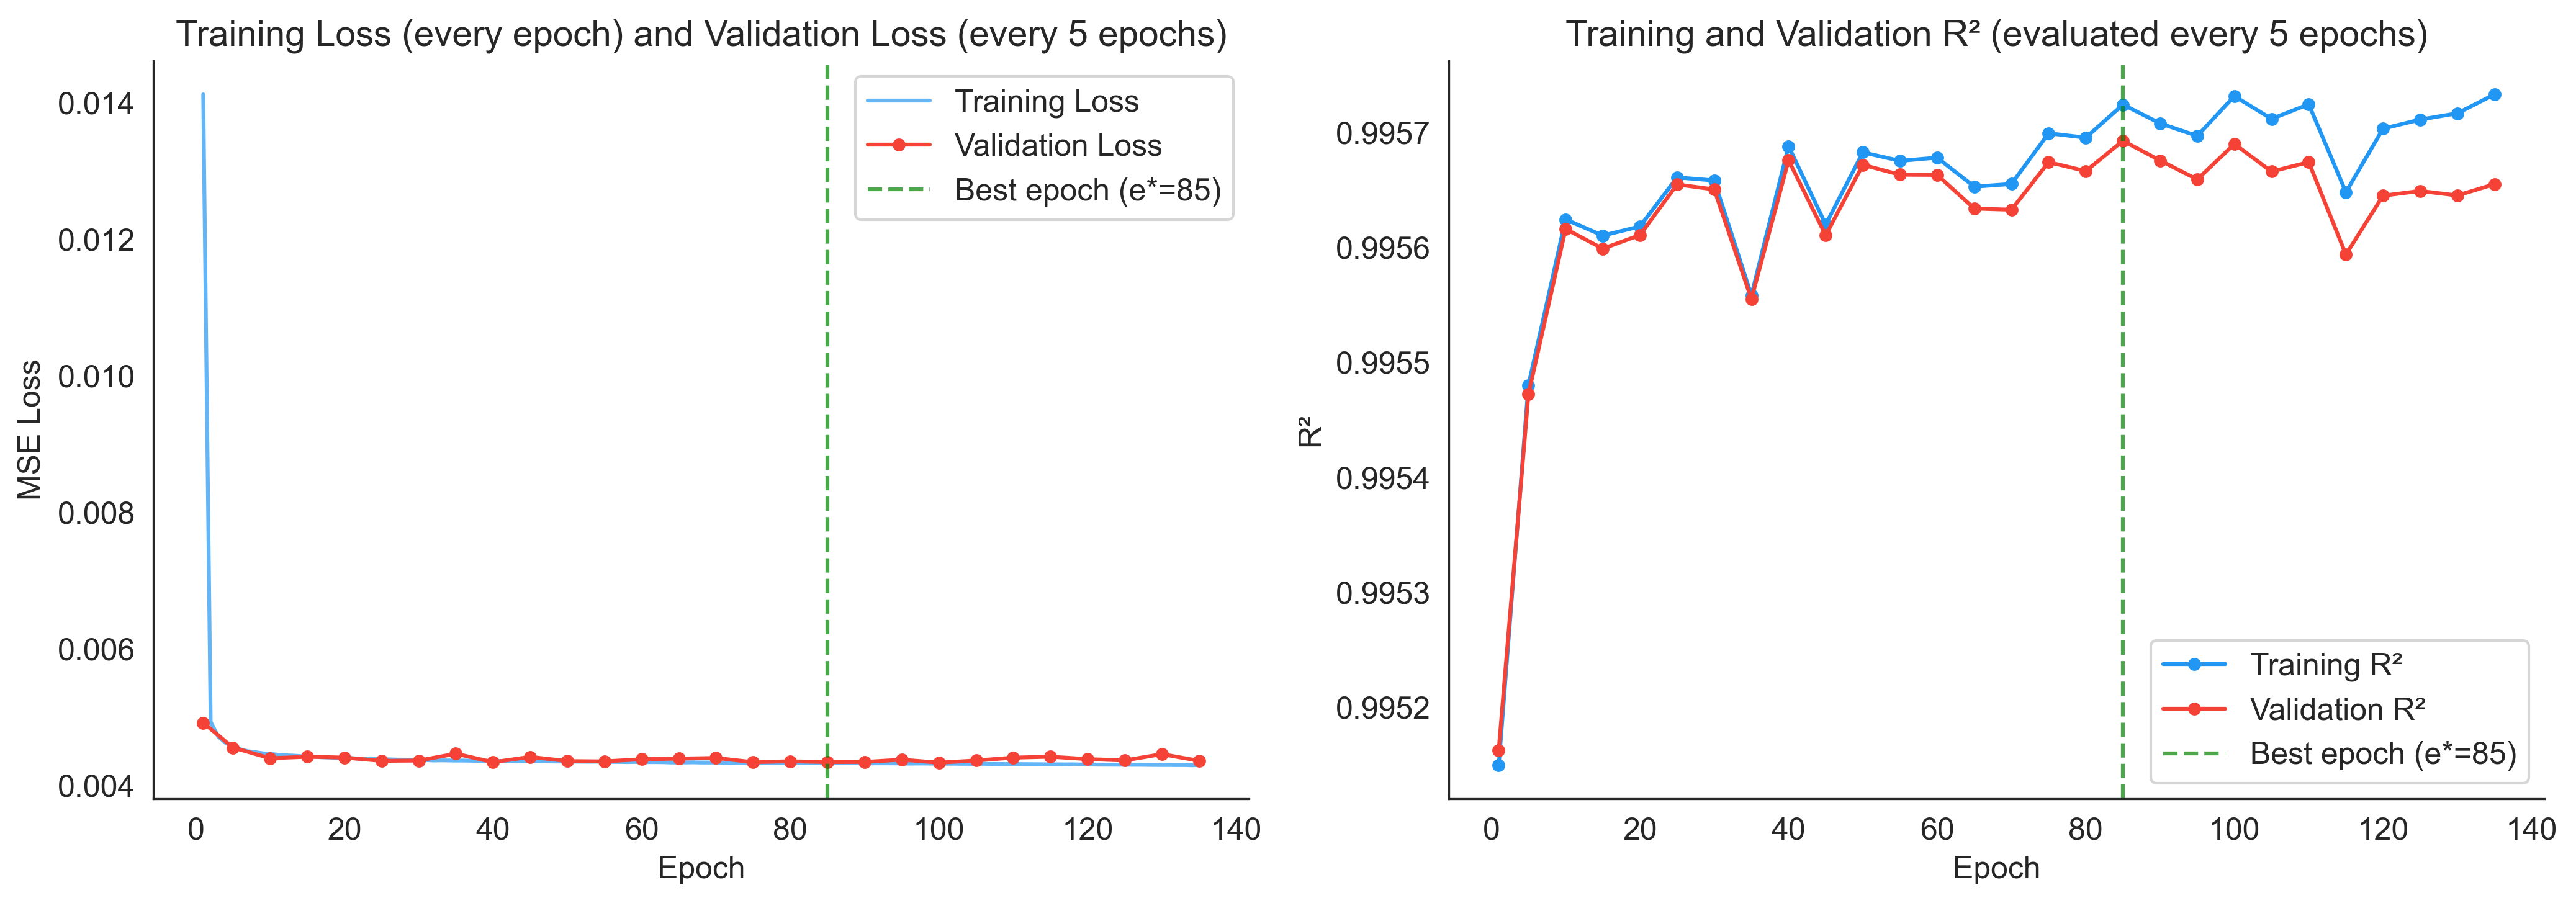
\includegraphics[width=0.90\textwidth]{Thesis/Chapter 3/Figures/fig_training_validation_curves.png}
    \caption{Training and validation loss with $R^2$ over epochs.}
    \label{fig:learning_curves_ch3}
\end{subfigure}

\vspace{0.4cm}

\begin{subfigure}[b]{\textwidth}
    \centering
    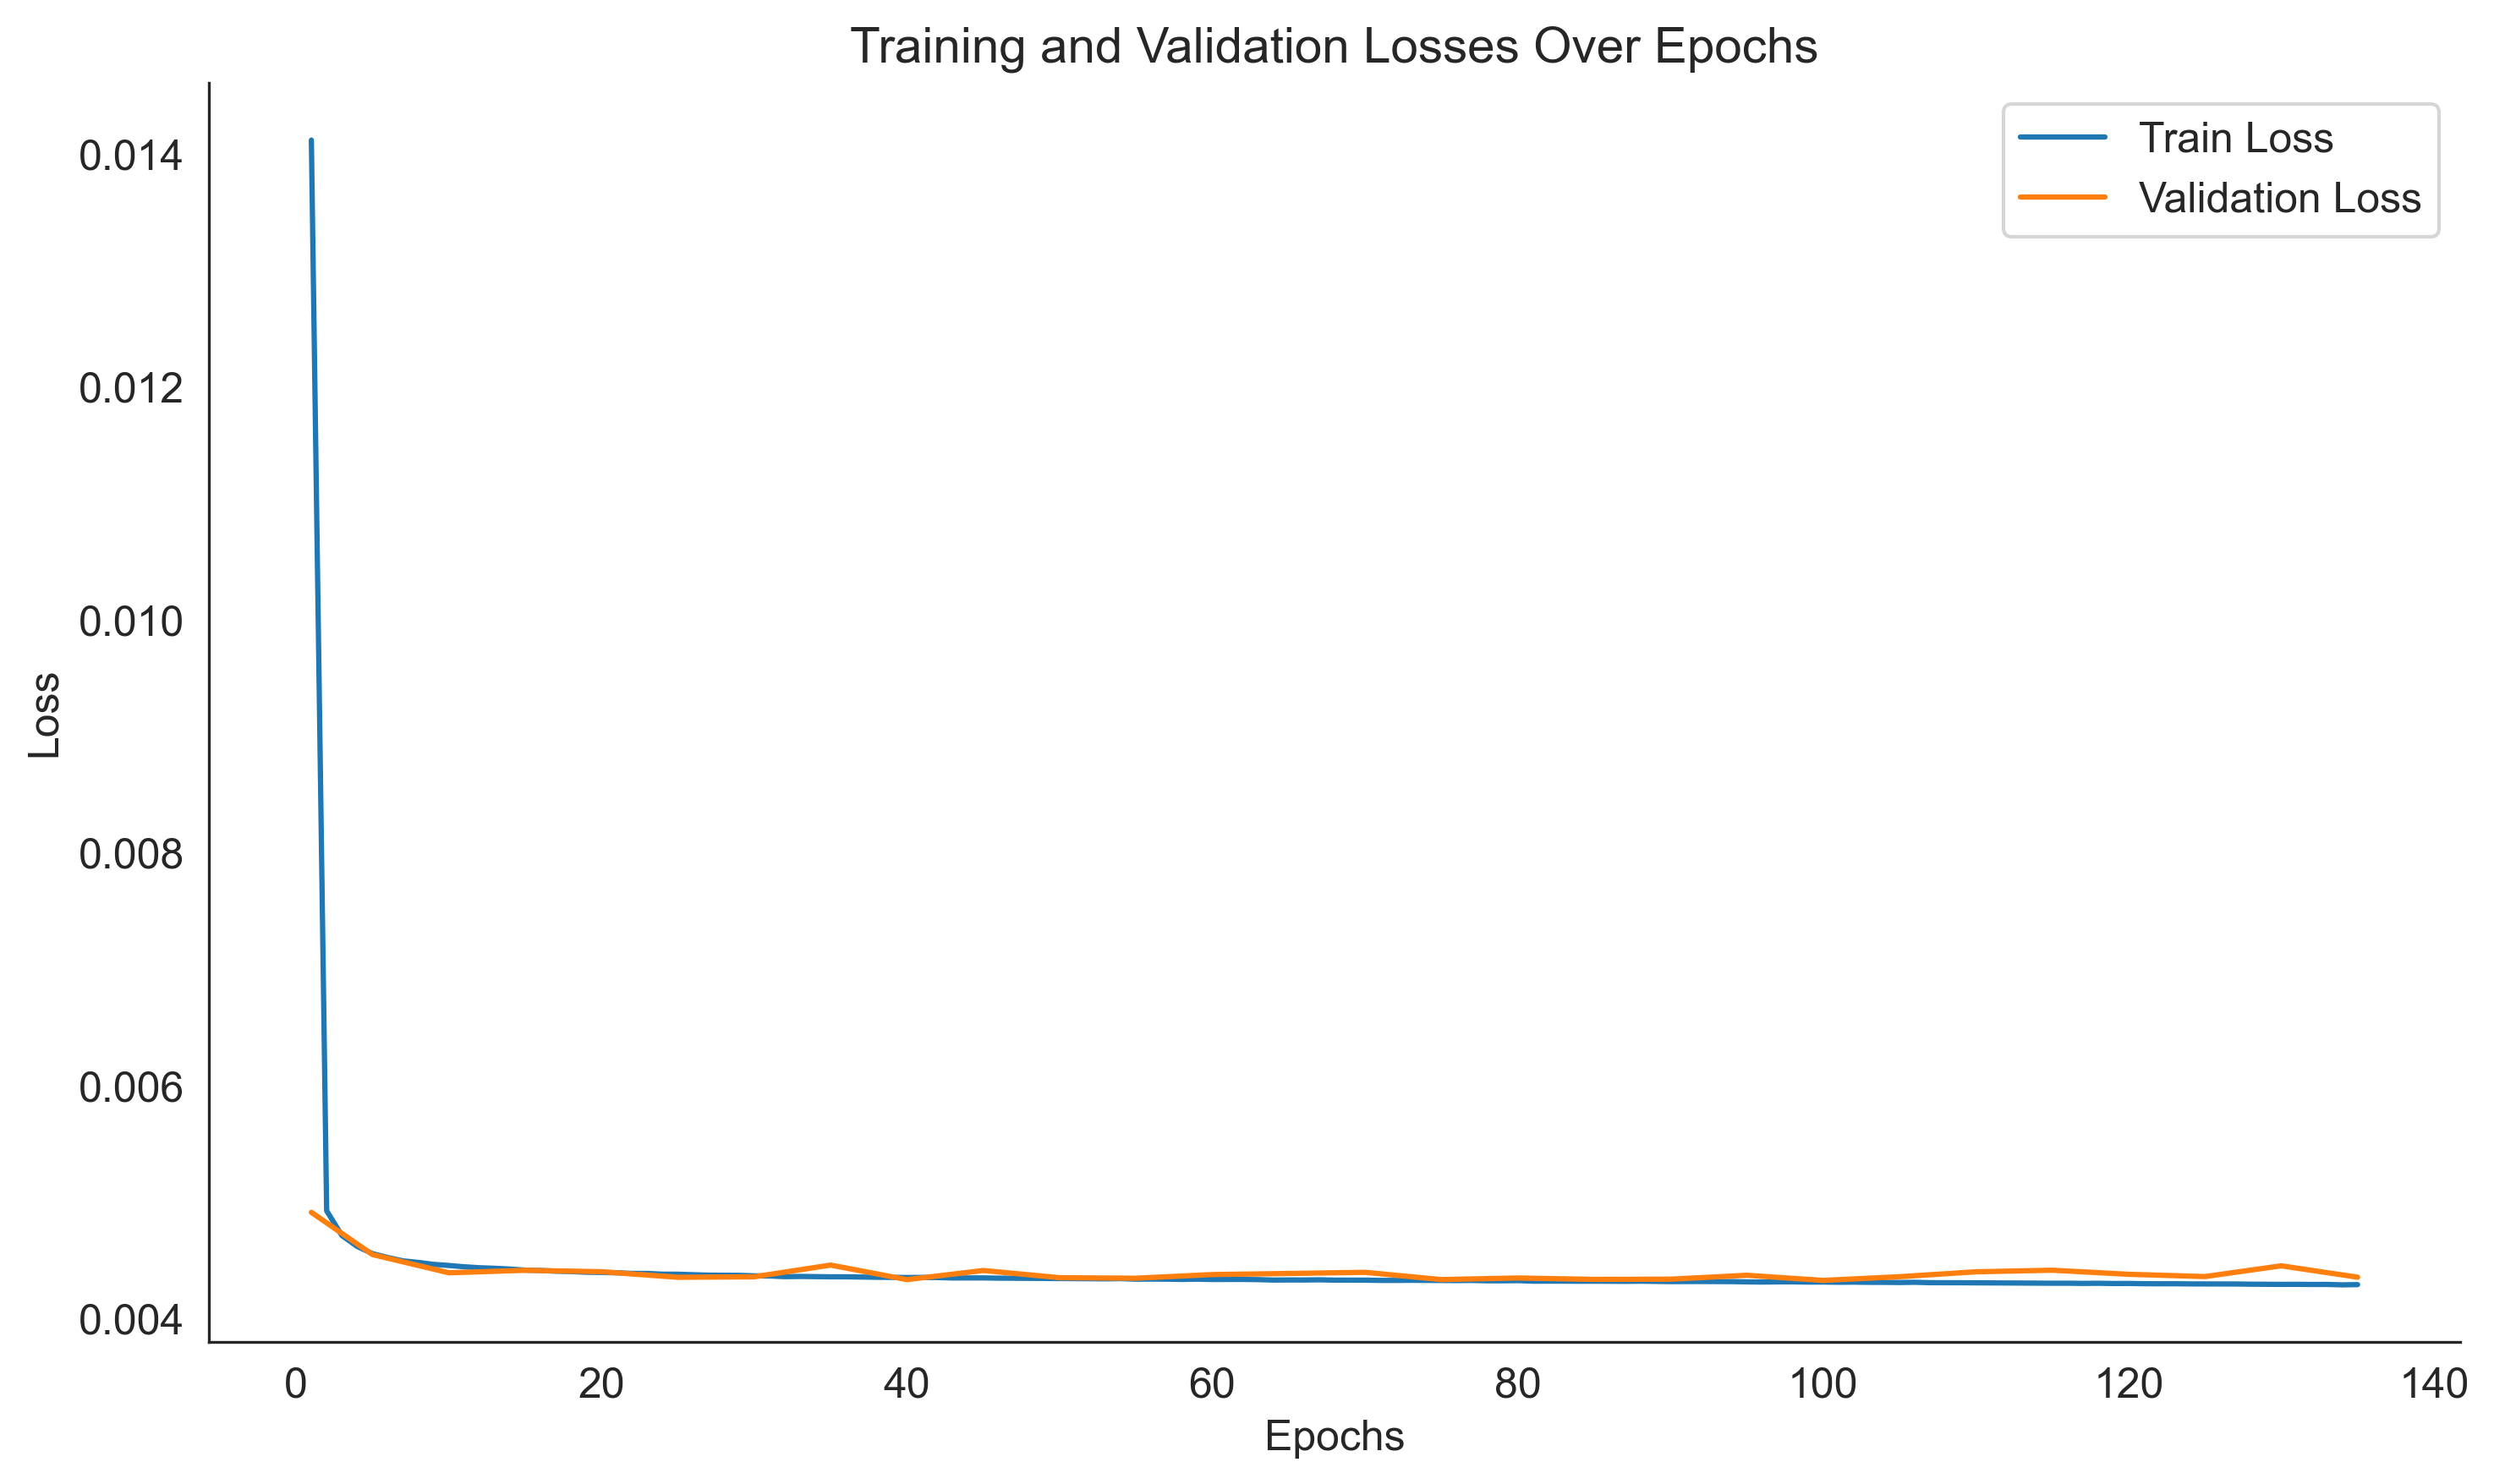
\includegraphics[width=0.90\textwidth]{Thesis/Chapter 3/Figures/fig_train_val_losses_epochs.png}
    \caption{Training and validation \gls{mse} losses over epochs for the final model.}
    \label{fig:train_val_losses_ch3}
\end{subfigure}
\caption{Learning curves for the fitted \gls{dnn}.}
\label{fig:learning_curves_combined_ch3}
\end{figure}

\noindent
Figure~\ref{fig:learning_curves_ch3} presents the learning curves for the
fitted \gls{dnn}. In the left panel, the training \gls{mse} loss drops sharply from
approximately 0.014 at the first epoch to roughly 0.005 by epoch~5, after
which it decreases gradually and stabilises near 0.0043. The validation \gls{mse}
loss tracks the training loss closely throughout, with no visible
divergence between the two curves. The selected epoch $e^{*} = 85$ (green
dashed line) falls in the region where both losses have plateaued. In the
right panel, both training and validation $R^2$ values rise rapidly from
approximately 0.9951 to a plateau near 0.9957, with the gap between them
remaining negligible. Figure~\ref{fig:train_val_losses_ch3} provides a
complementary view: the training loss (blue) exhibits a single spike at
epoch~1, consistent with random weight initialisation, before converging
rapidly, and the validation loss (orange) overlaps with it from epoch~20
onwards. The absence of any sustained divergence confirms stable
convergence without overfitting.

\subsubsection{Actual versus predicted diagnostics}

Two graphical summaries are used to compare observed charges with fitted
predictions.  First, the observed values $y_i$ are plotted directly
against the fitted values $\widehat{y}_i$ with a $45^\circ$ reference
line.  Second, observations are sorted by their observed charge, and the
actual and predicted values are displayed as overlaid curves; a well-fitted
model produces a predicted curve that closely tracks the actual curve across
the full range of the response.  Both diagnostics are produced separately
for the training, validation and test partitions, and together they indicate
whether the fitted model behaves differently in low-, central- and
high-cost regions.

\begin{figure}[H]
\centering
\begin{subfigure}[b]{0.48\textwidth}
    \centering
    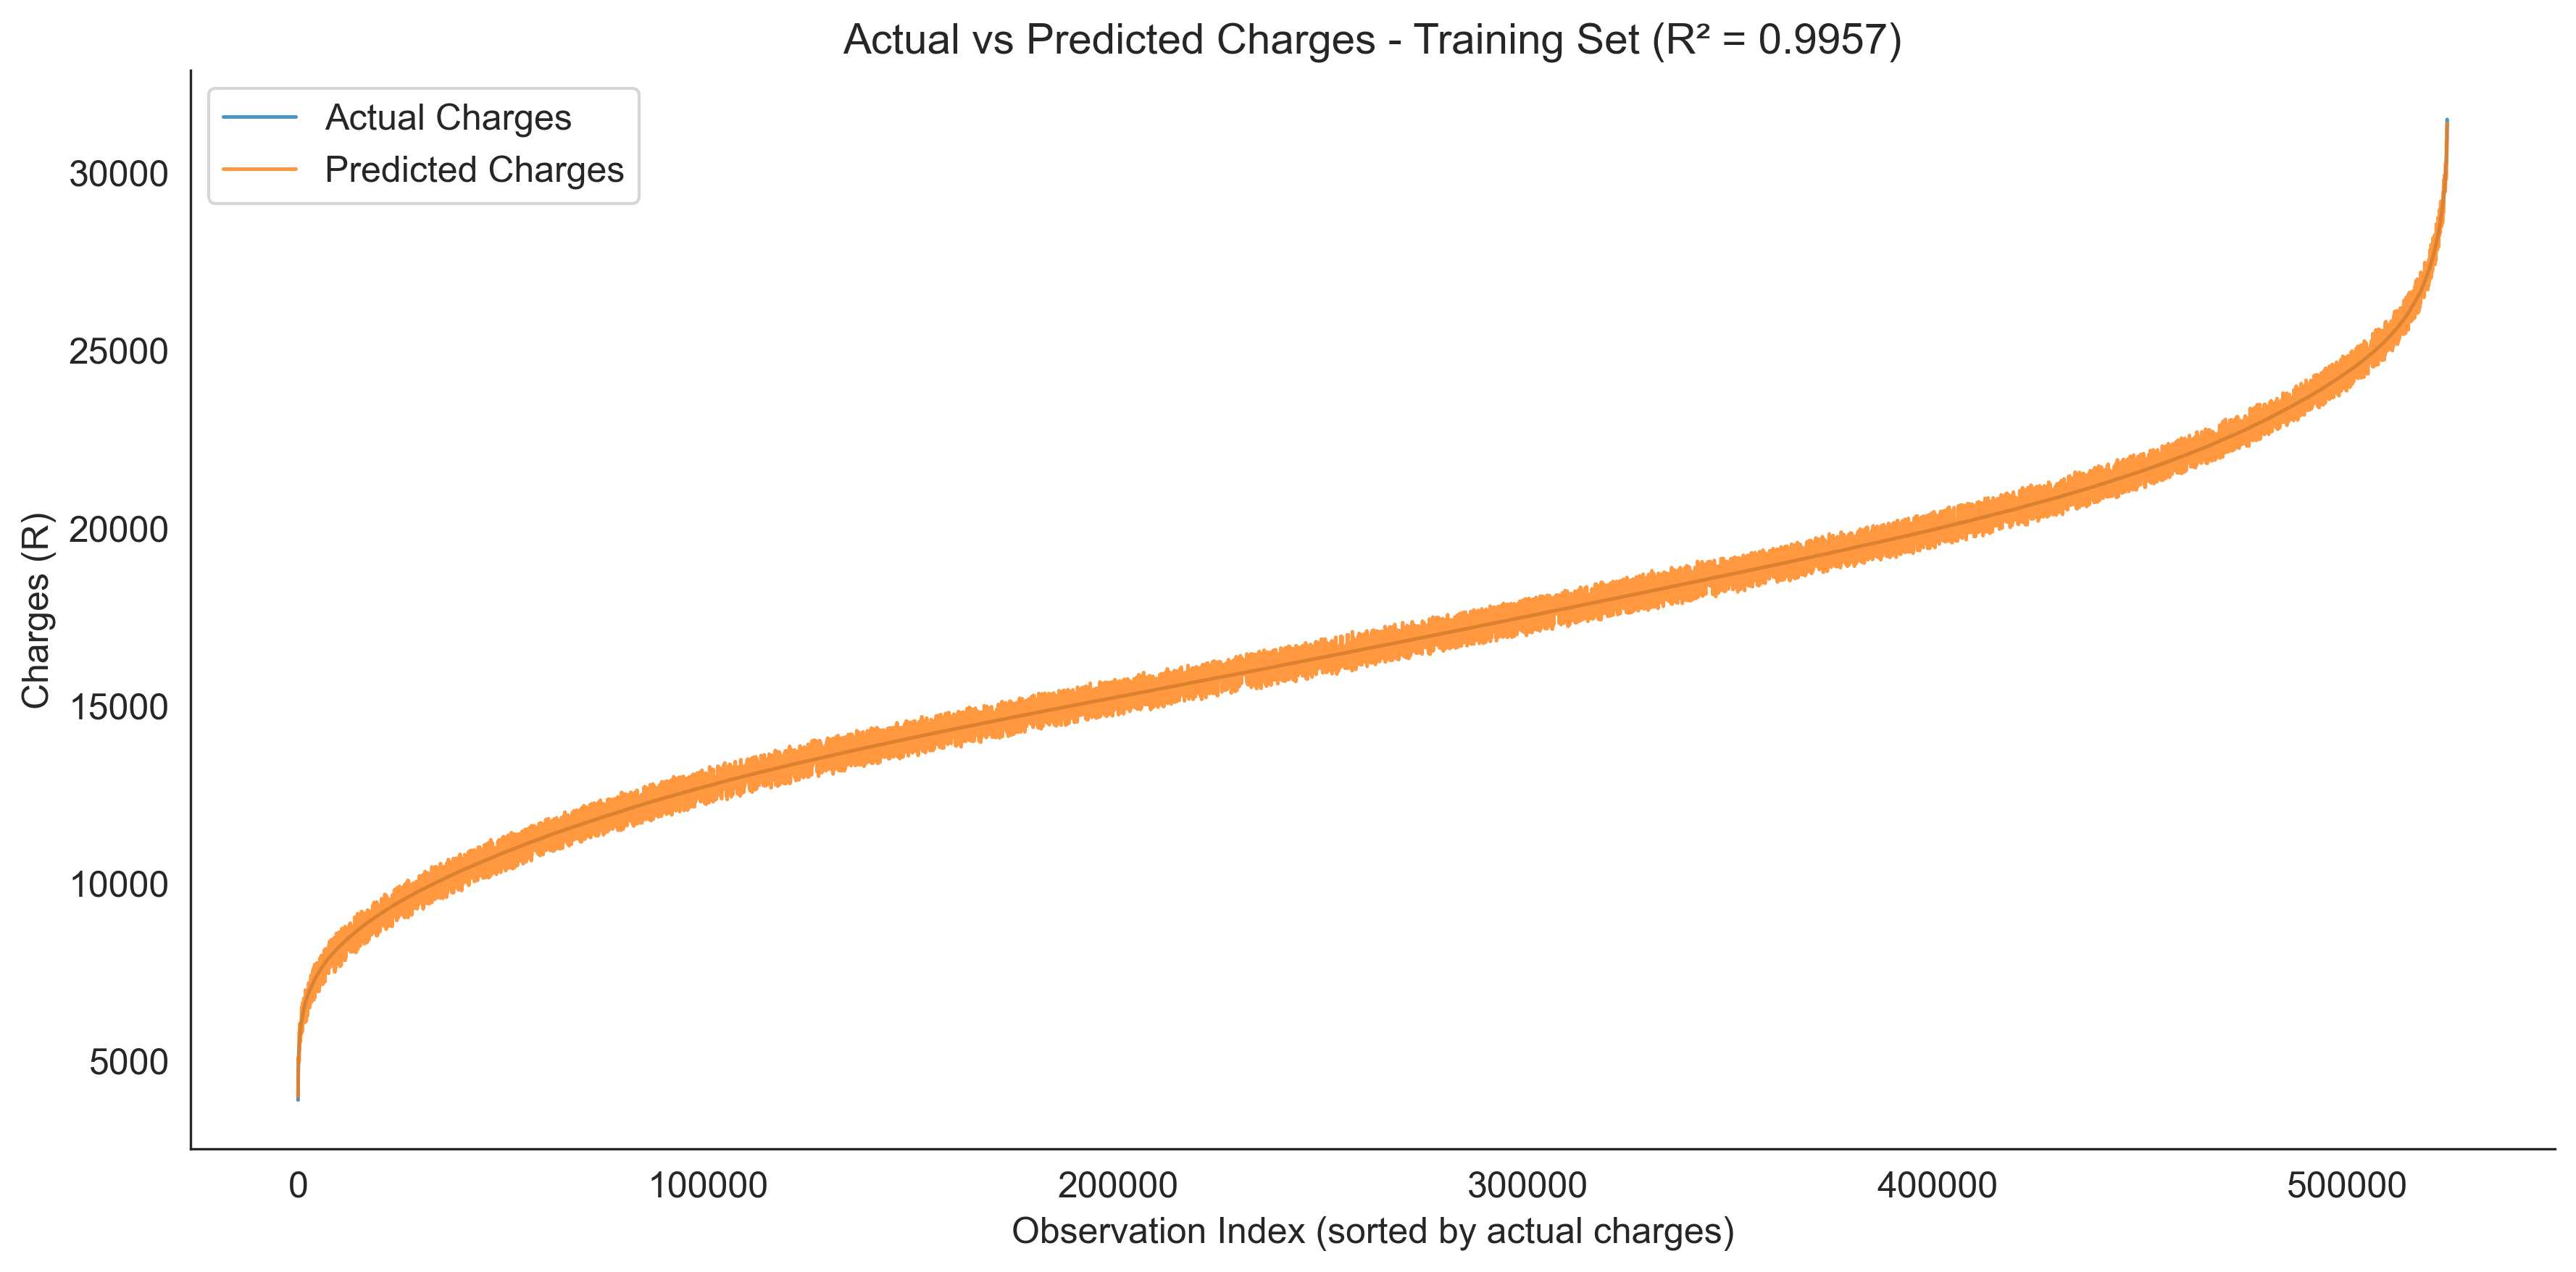
\includegraphics[width=\textwidth]{Thesis/Chapter 3/Figures/fig_actual_vs_predicted_sorted_train.png}
    \caption{Training set ($R^2 = 0.9957$).}
    \label{fig:actual_vs_predicted_train_ch3}
\end{subfigure}
\hfill
\begin{subfigure}[b]{0.48\textwidth}
    \centering
    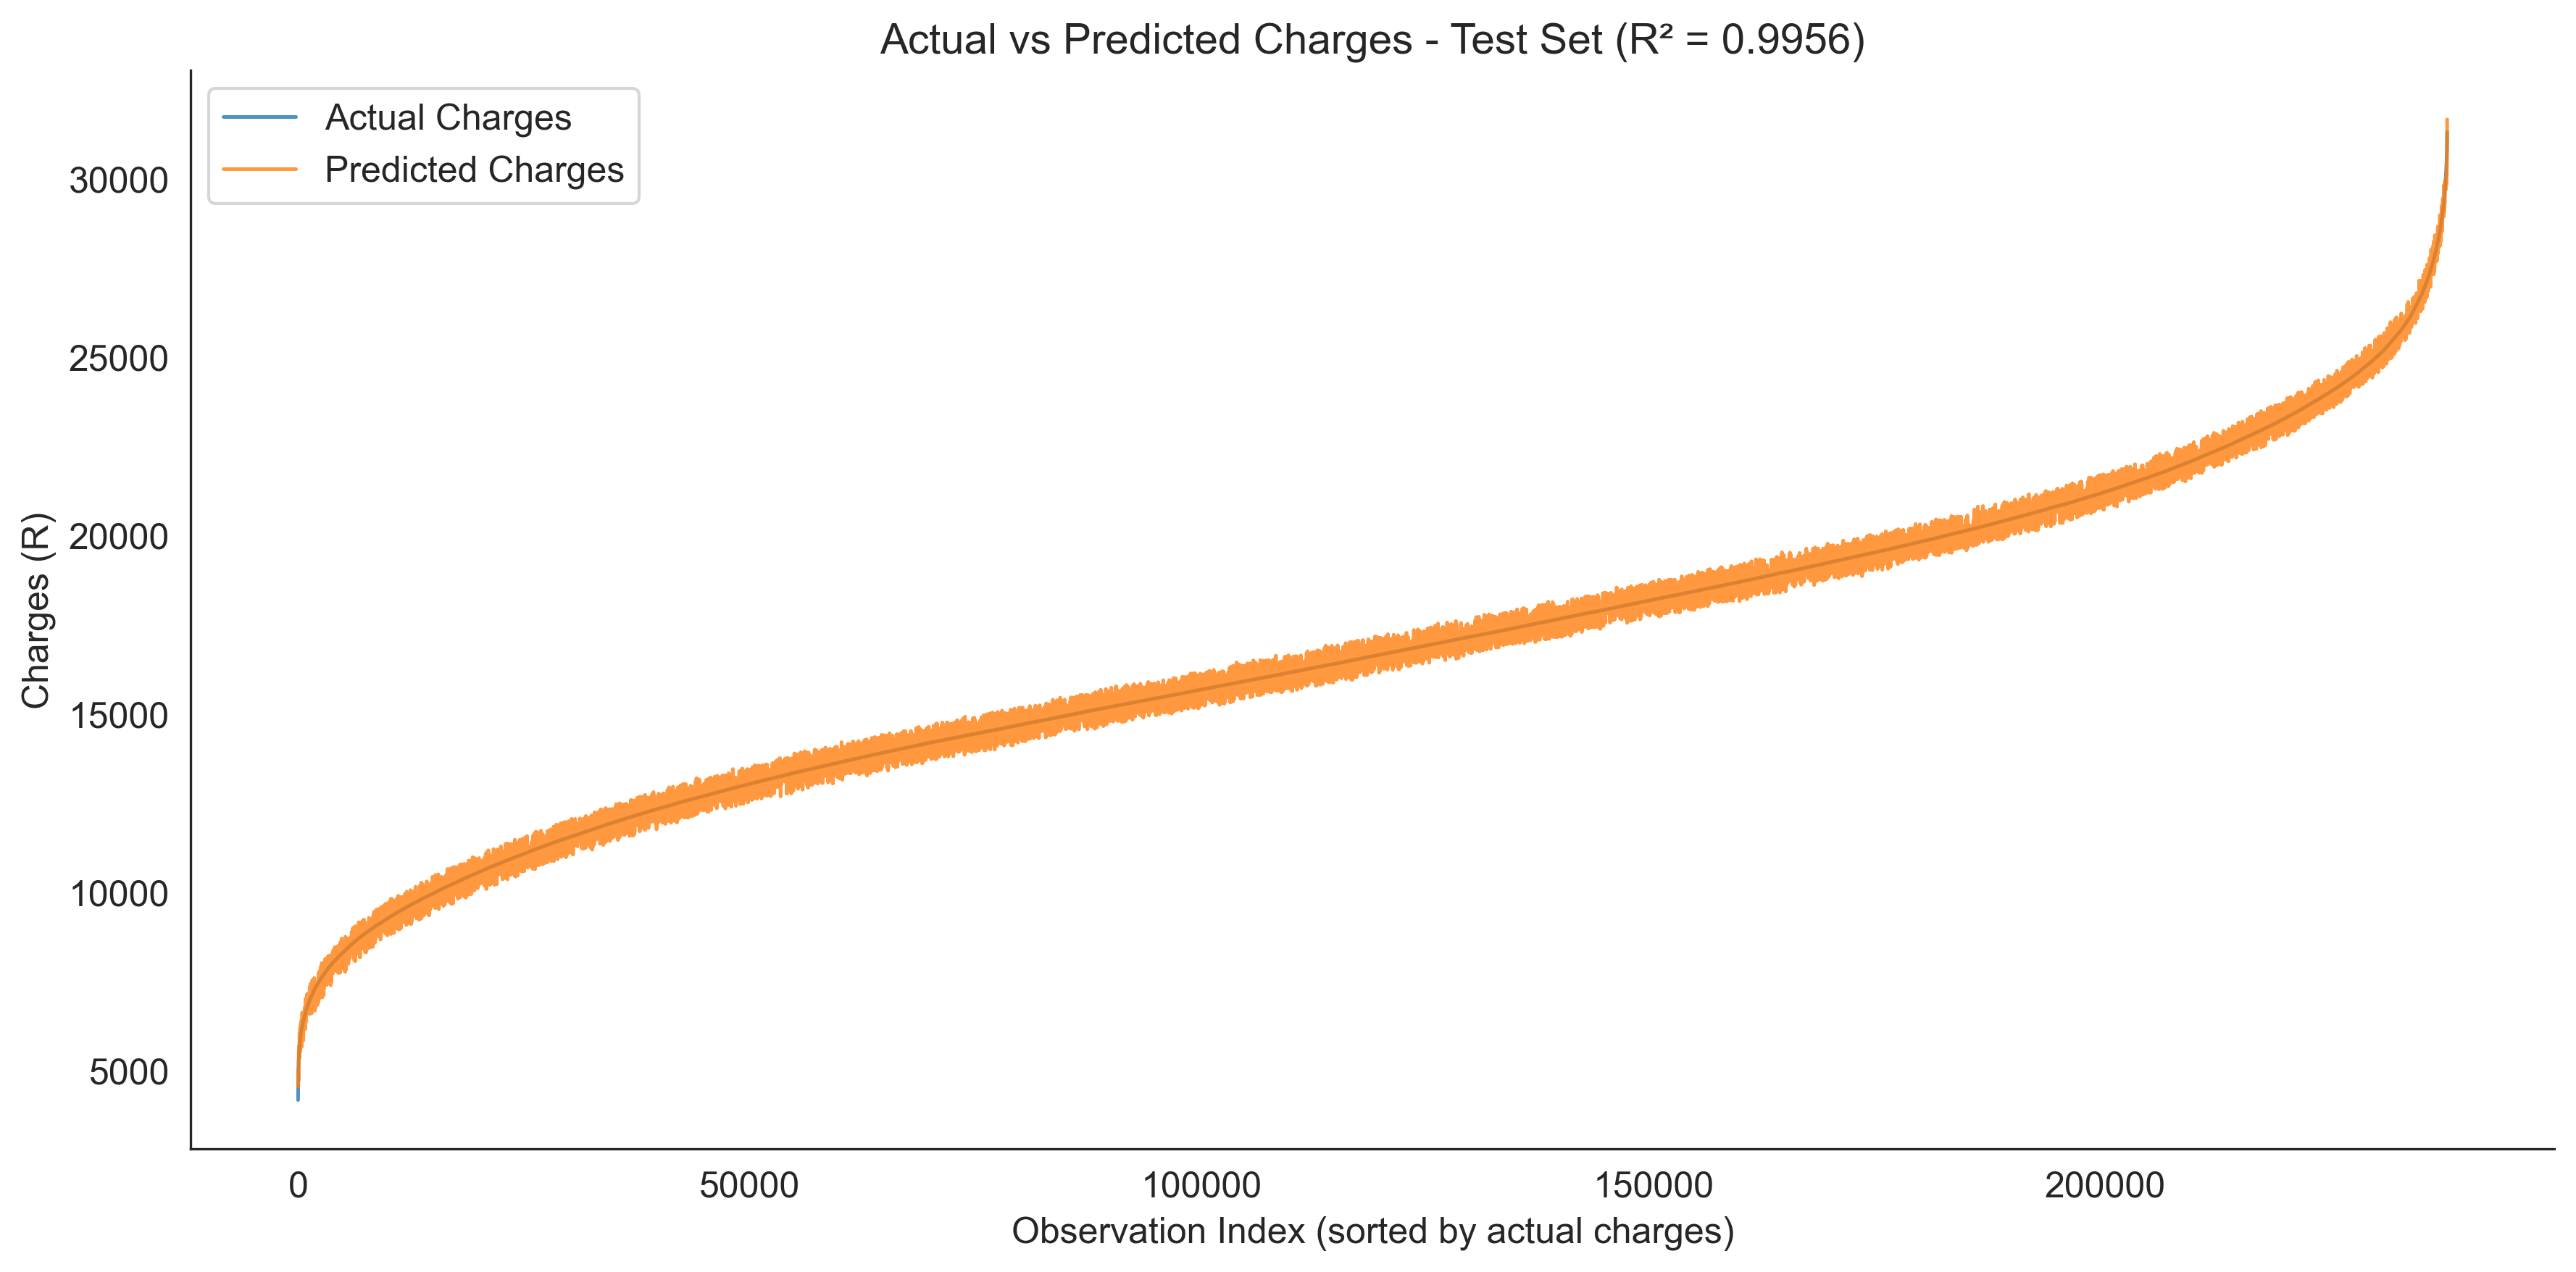
\includegraphics[width=\textwidth]{Thesis/Chapter 3/Figures/fig_actual_vs_predicted_sorted_test.png}
    \caption{Test set ($R^2 = 0.9956$).}
    \label{fig:actual_vs_predicted_test_ch3}
\end{subfigure}
\caption{Sorted actual versus predicted charges on training and test sets.}
\label{fig:actual_vs_predicted_ch3}
\end{figure}

\noindent
Figure~\ref{fig:actual_vs_predicted_ch3} shows the sorted actual versus
predicted charges on both partitions. In the training set
(Figure~\ref{fig:actual_vs_predicted_train_ch3}), the predicted line
(orange) tracks the actual line (blue) so closely that the two are nearly
indistinguishable across the full range of the response, from approximately
R4\,000 at the lower end to R32\,000 at the upper end. A modest increase
in prediction scatter is visible in the upper tail above R25\,000, but the
deviations remain small relative to the response scale. The test set
(Figure~\ref{fig:actual_vs_predicted_test_ch3}) displays a virtually
identical pattern. The negligible drop from training $R^2 = 0.9957$ to test
$R^2 = 0.9956$ confirms that the model generalises to unseen observations
without meaningful performance degradation.

\begin{figure}[H]
\centering
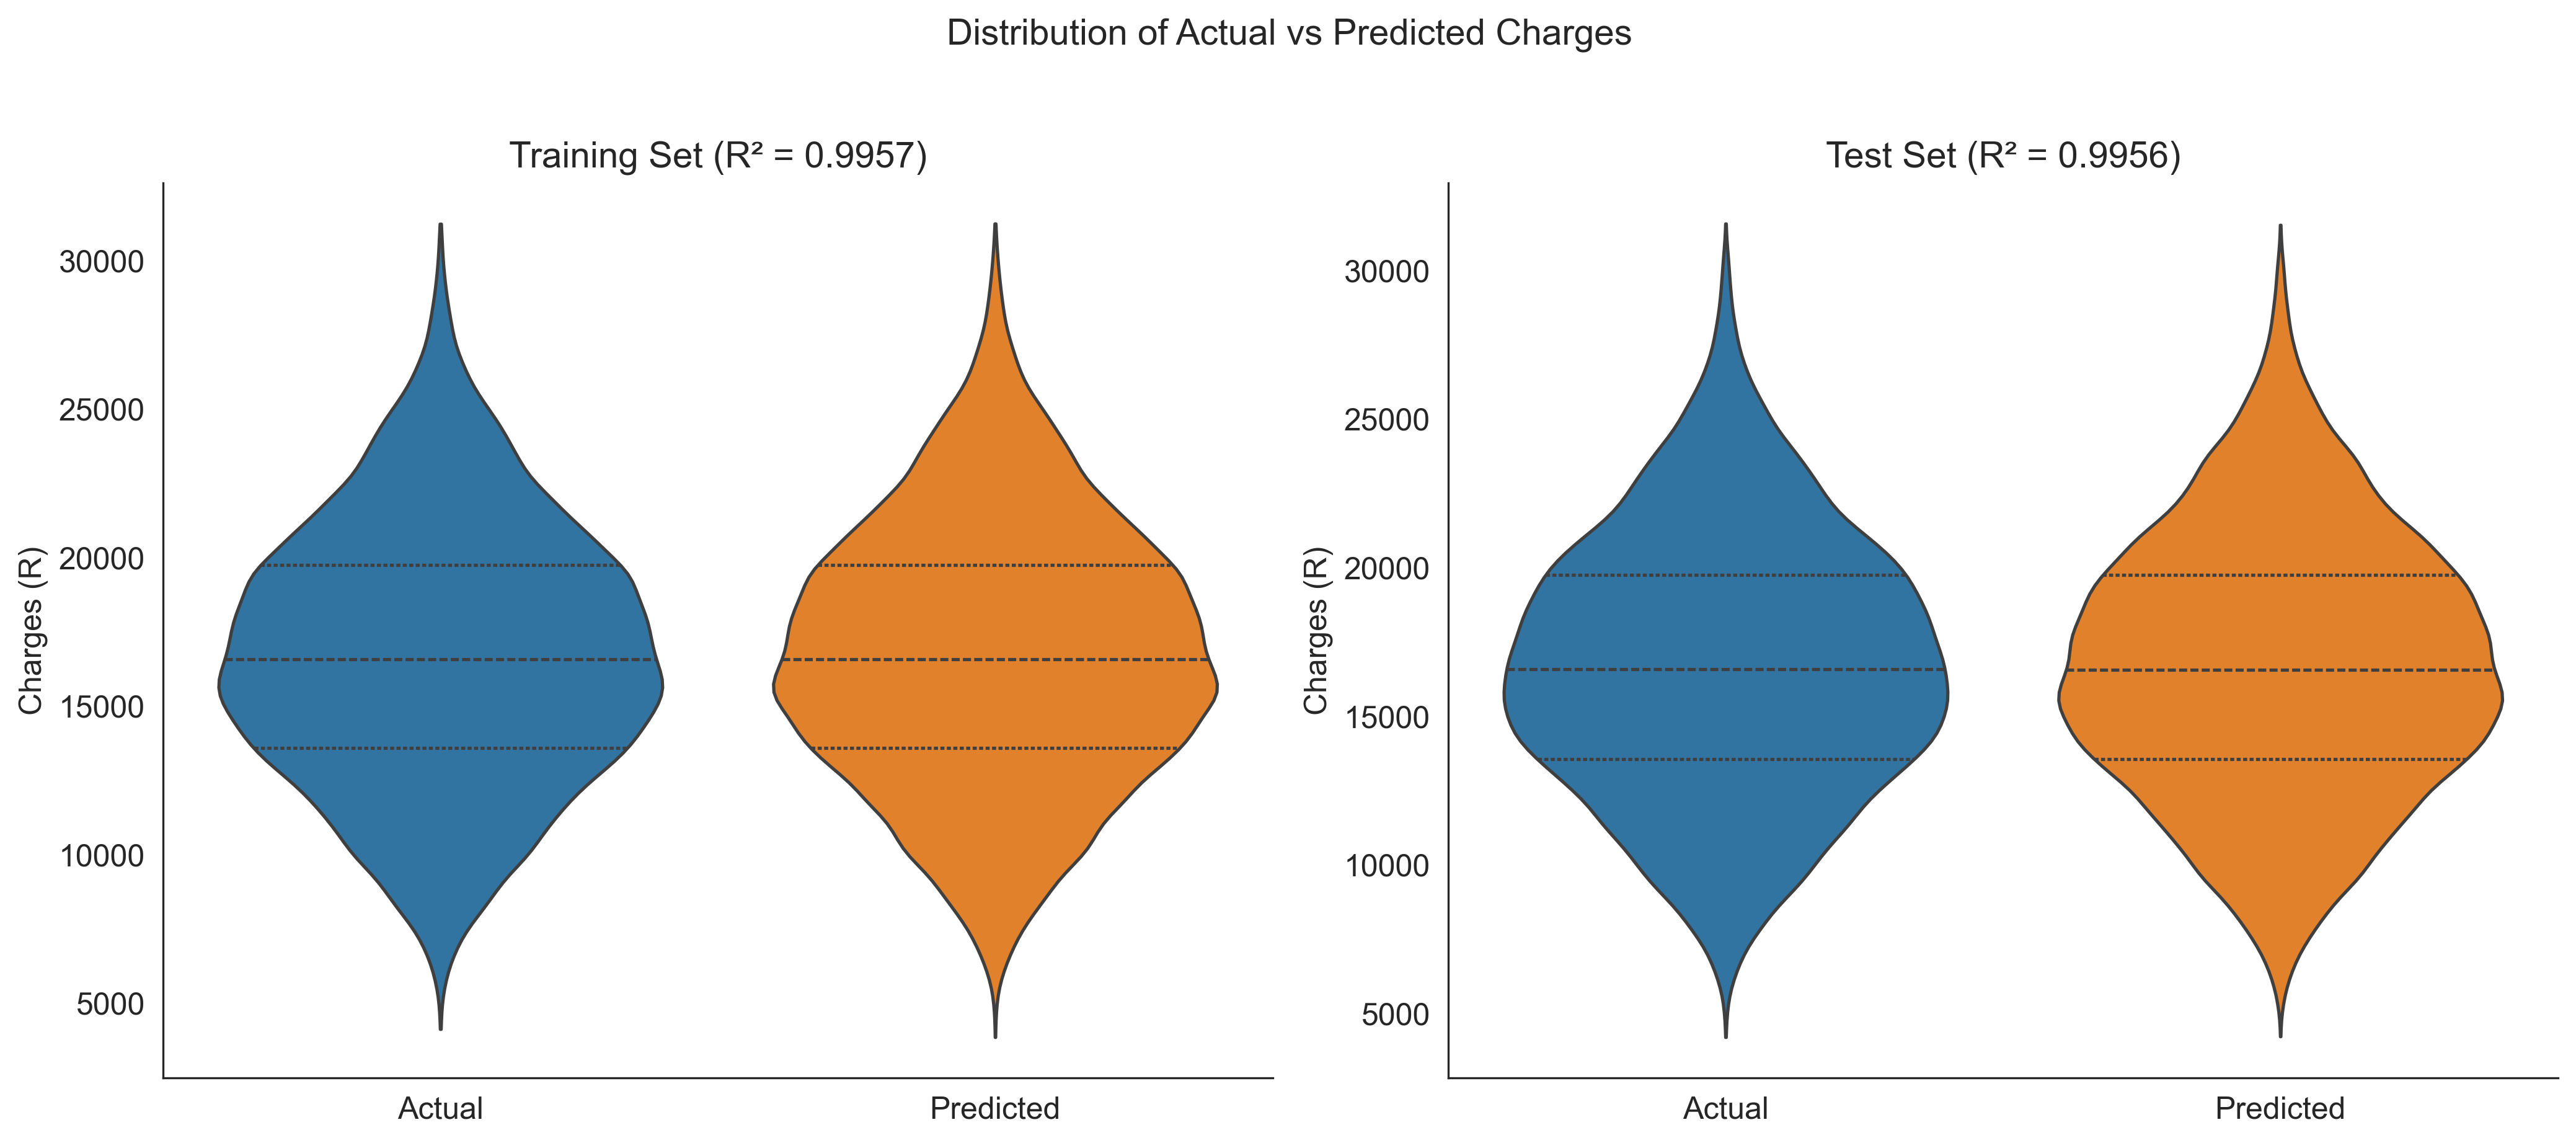
\includegraphics[width=0.90\textwidth]{Thesis/Chapter 3/Figures/fig_violin_actual_vs_predicted.png}
\caption{Violin plots of actual versus predicted charges on training and test sets.}
\label{fig:violin_actual_vs_predicted_ch3}
\end{figure}

\noindent
Figure~\ref{fig:violin_actual_vs_predicted_ch3} compares the distributional
profiles of actual and predicted charges on both partitions. In the
training set (left panel, $R^2 = 0.9957$), the actual (blue) and predicted
(orange) violins exhibit closely matching shapes: both are unimodal with
the bulk of density concentrated between approximately R10\,000 and
R25\,000, and the dashed median lines fall at approximately the same level
near R16\,700. The predicted violin is marginally narrower at the extreme
tails, indicating that the \gls{dnn} compresses the most extreme values slightly,
which is consistent with the smoothing behaviour of a regression model. The
test set (right panel, $R^2 = 0.9956$) displays the same pattern, with the
actual and predicted distributions virtually mirroring each other. The
consistency between training and test panels confirms that the model's
distributional calibration is preserved on unseen data.

\subsubsection{Residual diagnostics}

Residual diagnostics examine whether prediction errors contain systematic
structure.  Using the residuals defined in
equation~\eqref{eq:residual_definition_ch3}, the following plots are
produced:
\begin{enumerate}
    \item residuals versus fitted values, to detect systematic bias or
          changes in spread;
    \item a residual histogram, to assess the empirical shape and centring
          of the prediction errors;
    \item a $Q\text{-}Q$ plot of standardised residuals, to inspect tail
          behaviour;
    \item residuals versus observation index, to identify possible ordering
          or sequential patterns;
    \item residual distribution comparisons across the training, validation
          and test partitions.
\end{enumerate}
The \gls{dnn} does not require normally distributed residuals; these checks
are purely descriptive.  The fitted residuals are also retained for the
residual-augmented \gls{mc} sensitivity analysis described later.

\begin{figure}[H]
\centering
\begin{subfigure}[b]{\textwidth}
    \centering
    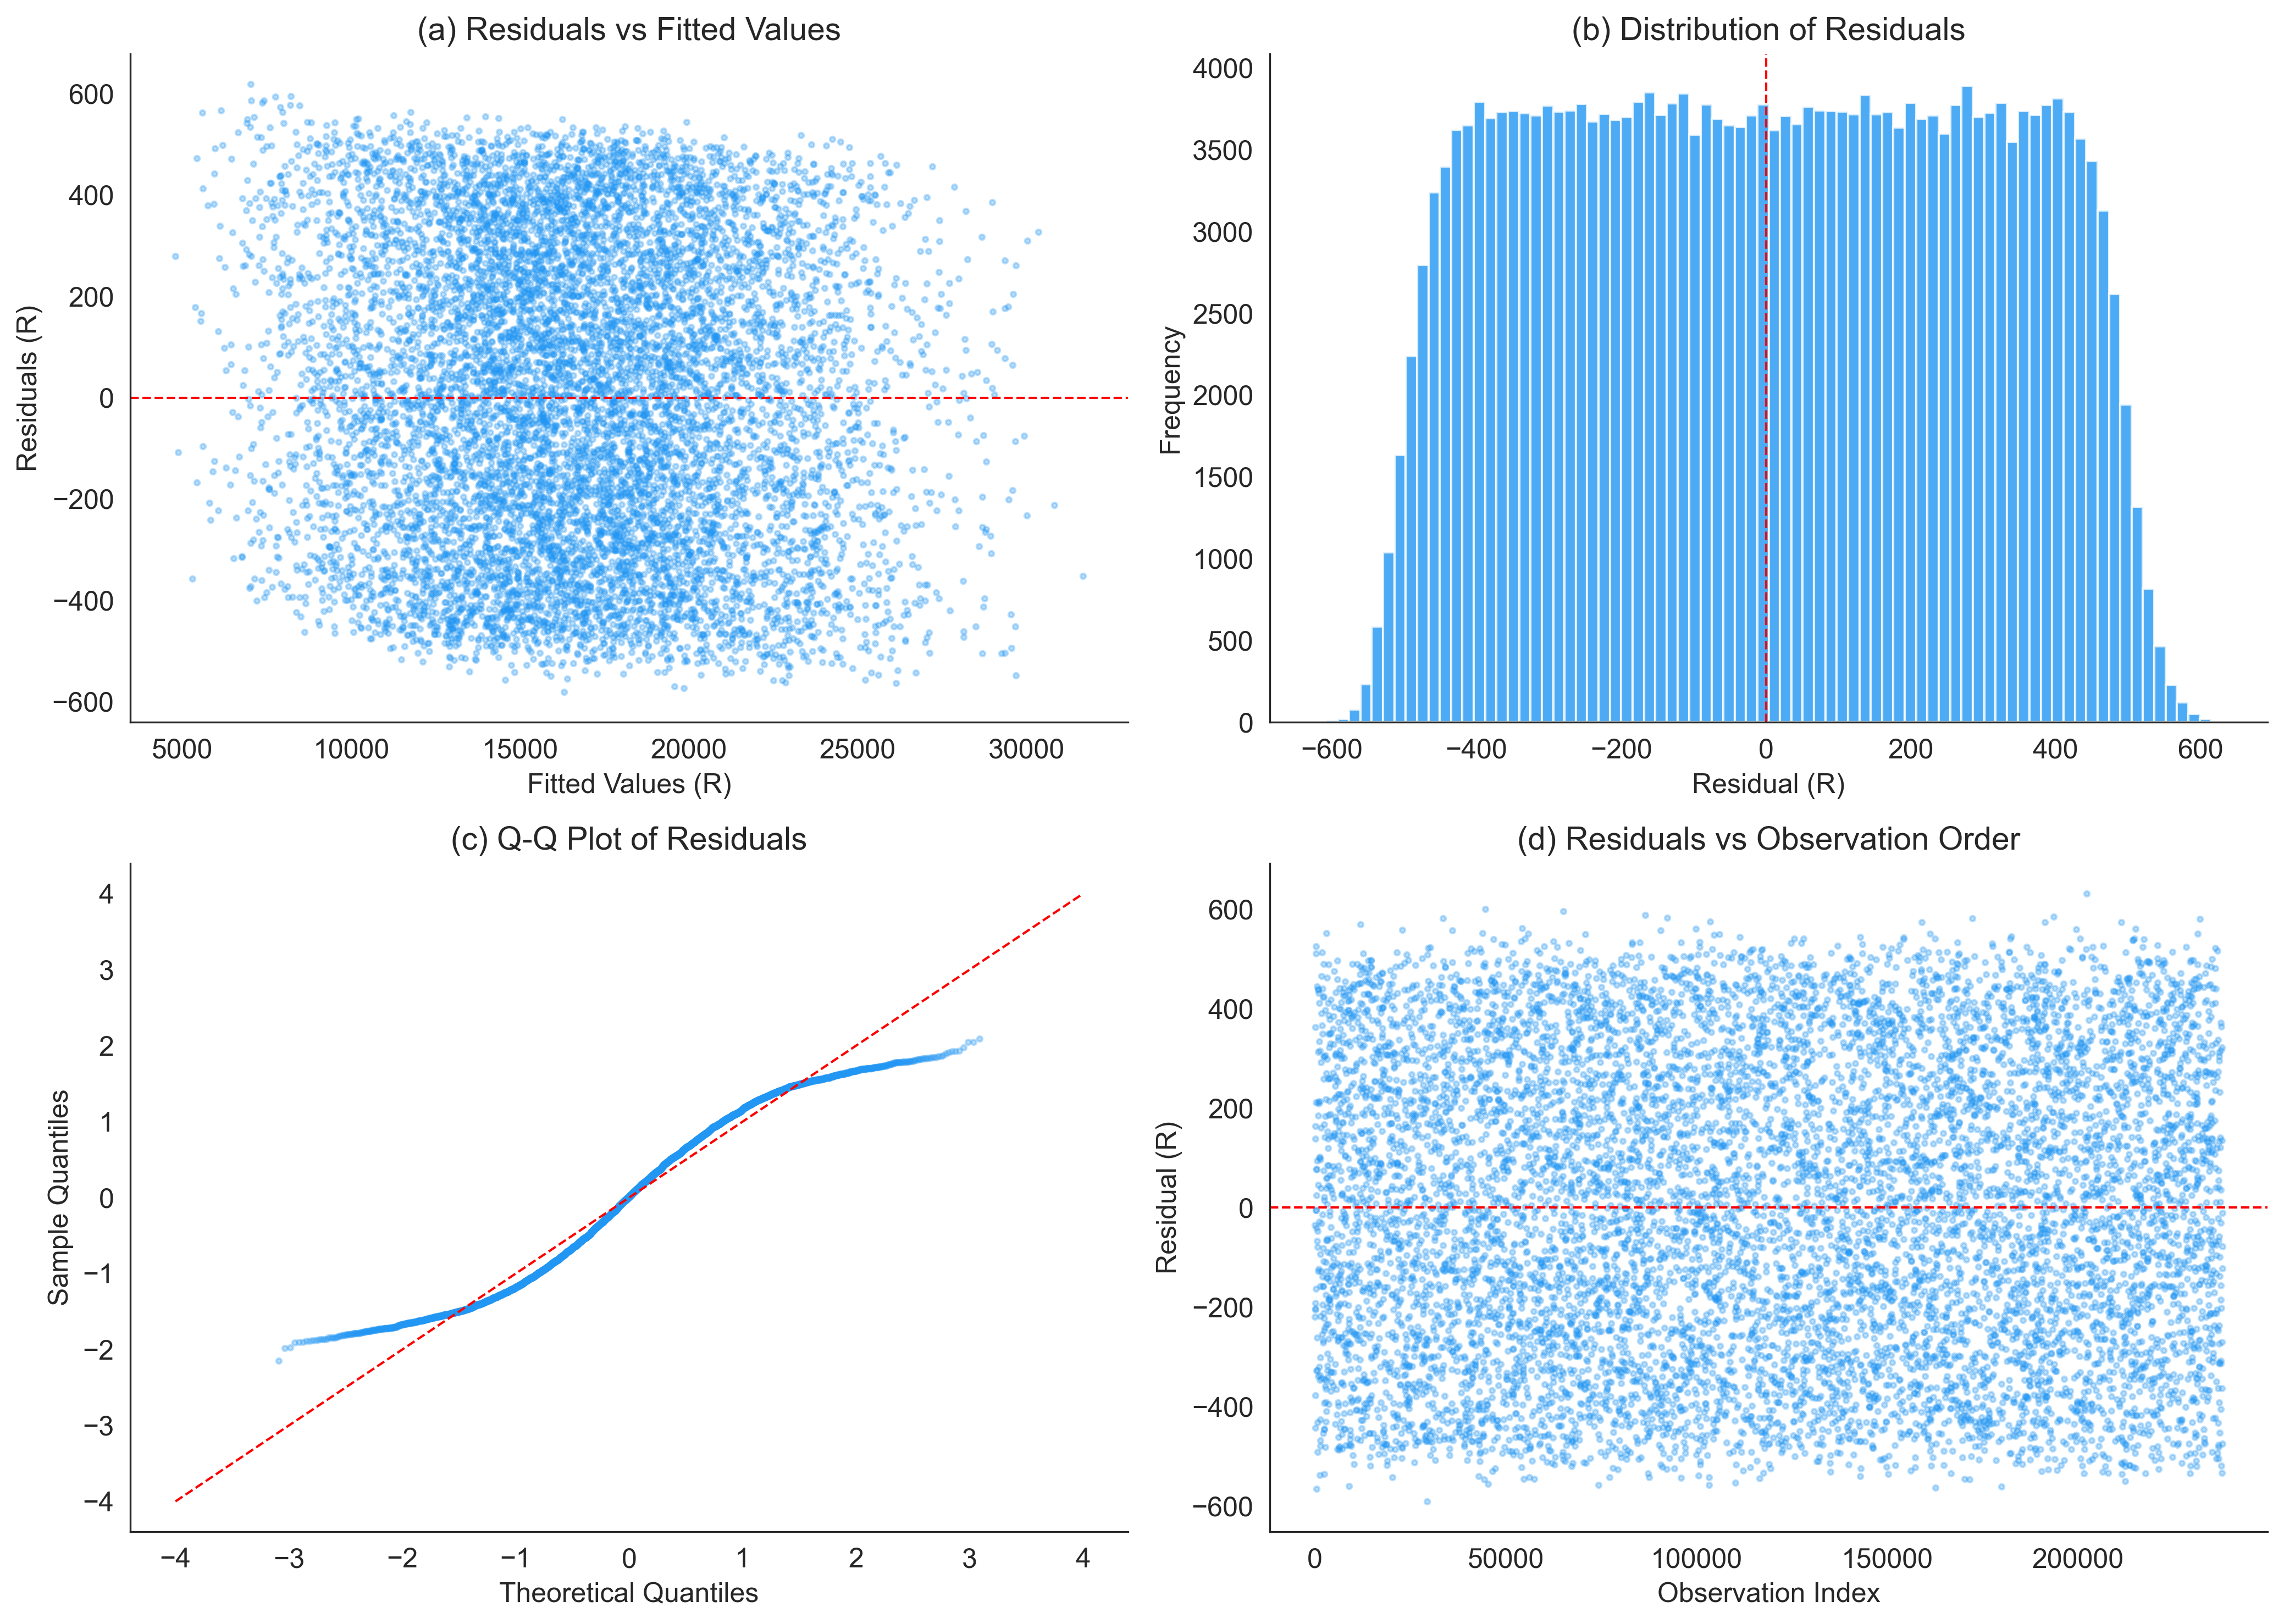
\includegraphics[width=0.90\textwidth]{Thesis/Chapter 3/Figures/fig_residual_diagnostics.png}
    \caption{Residual diagnostic panels for the fitted \gls{dnn}.}
    \label{fig:residual_diagnostics_ch3}
\end{subfigure}

\vspace{0.4cm}

\begin{subfigure}[b]{0.55\textwidth}
    \centering
    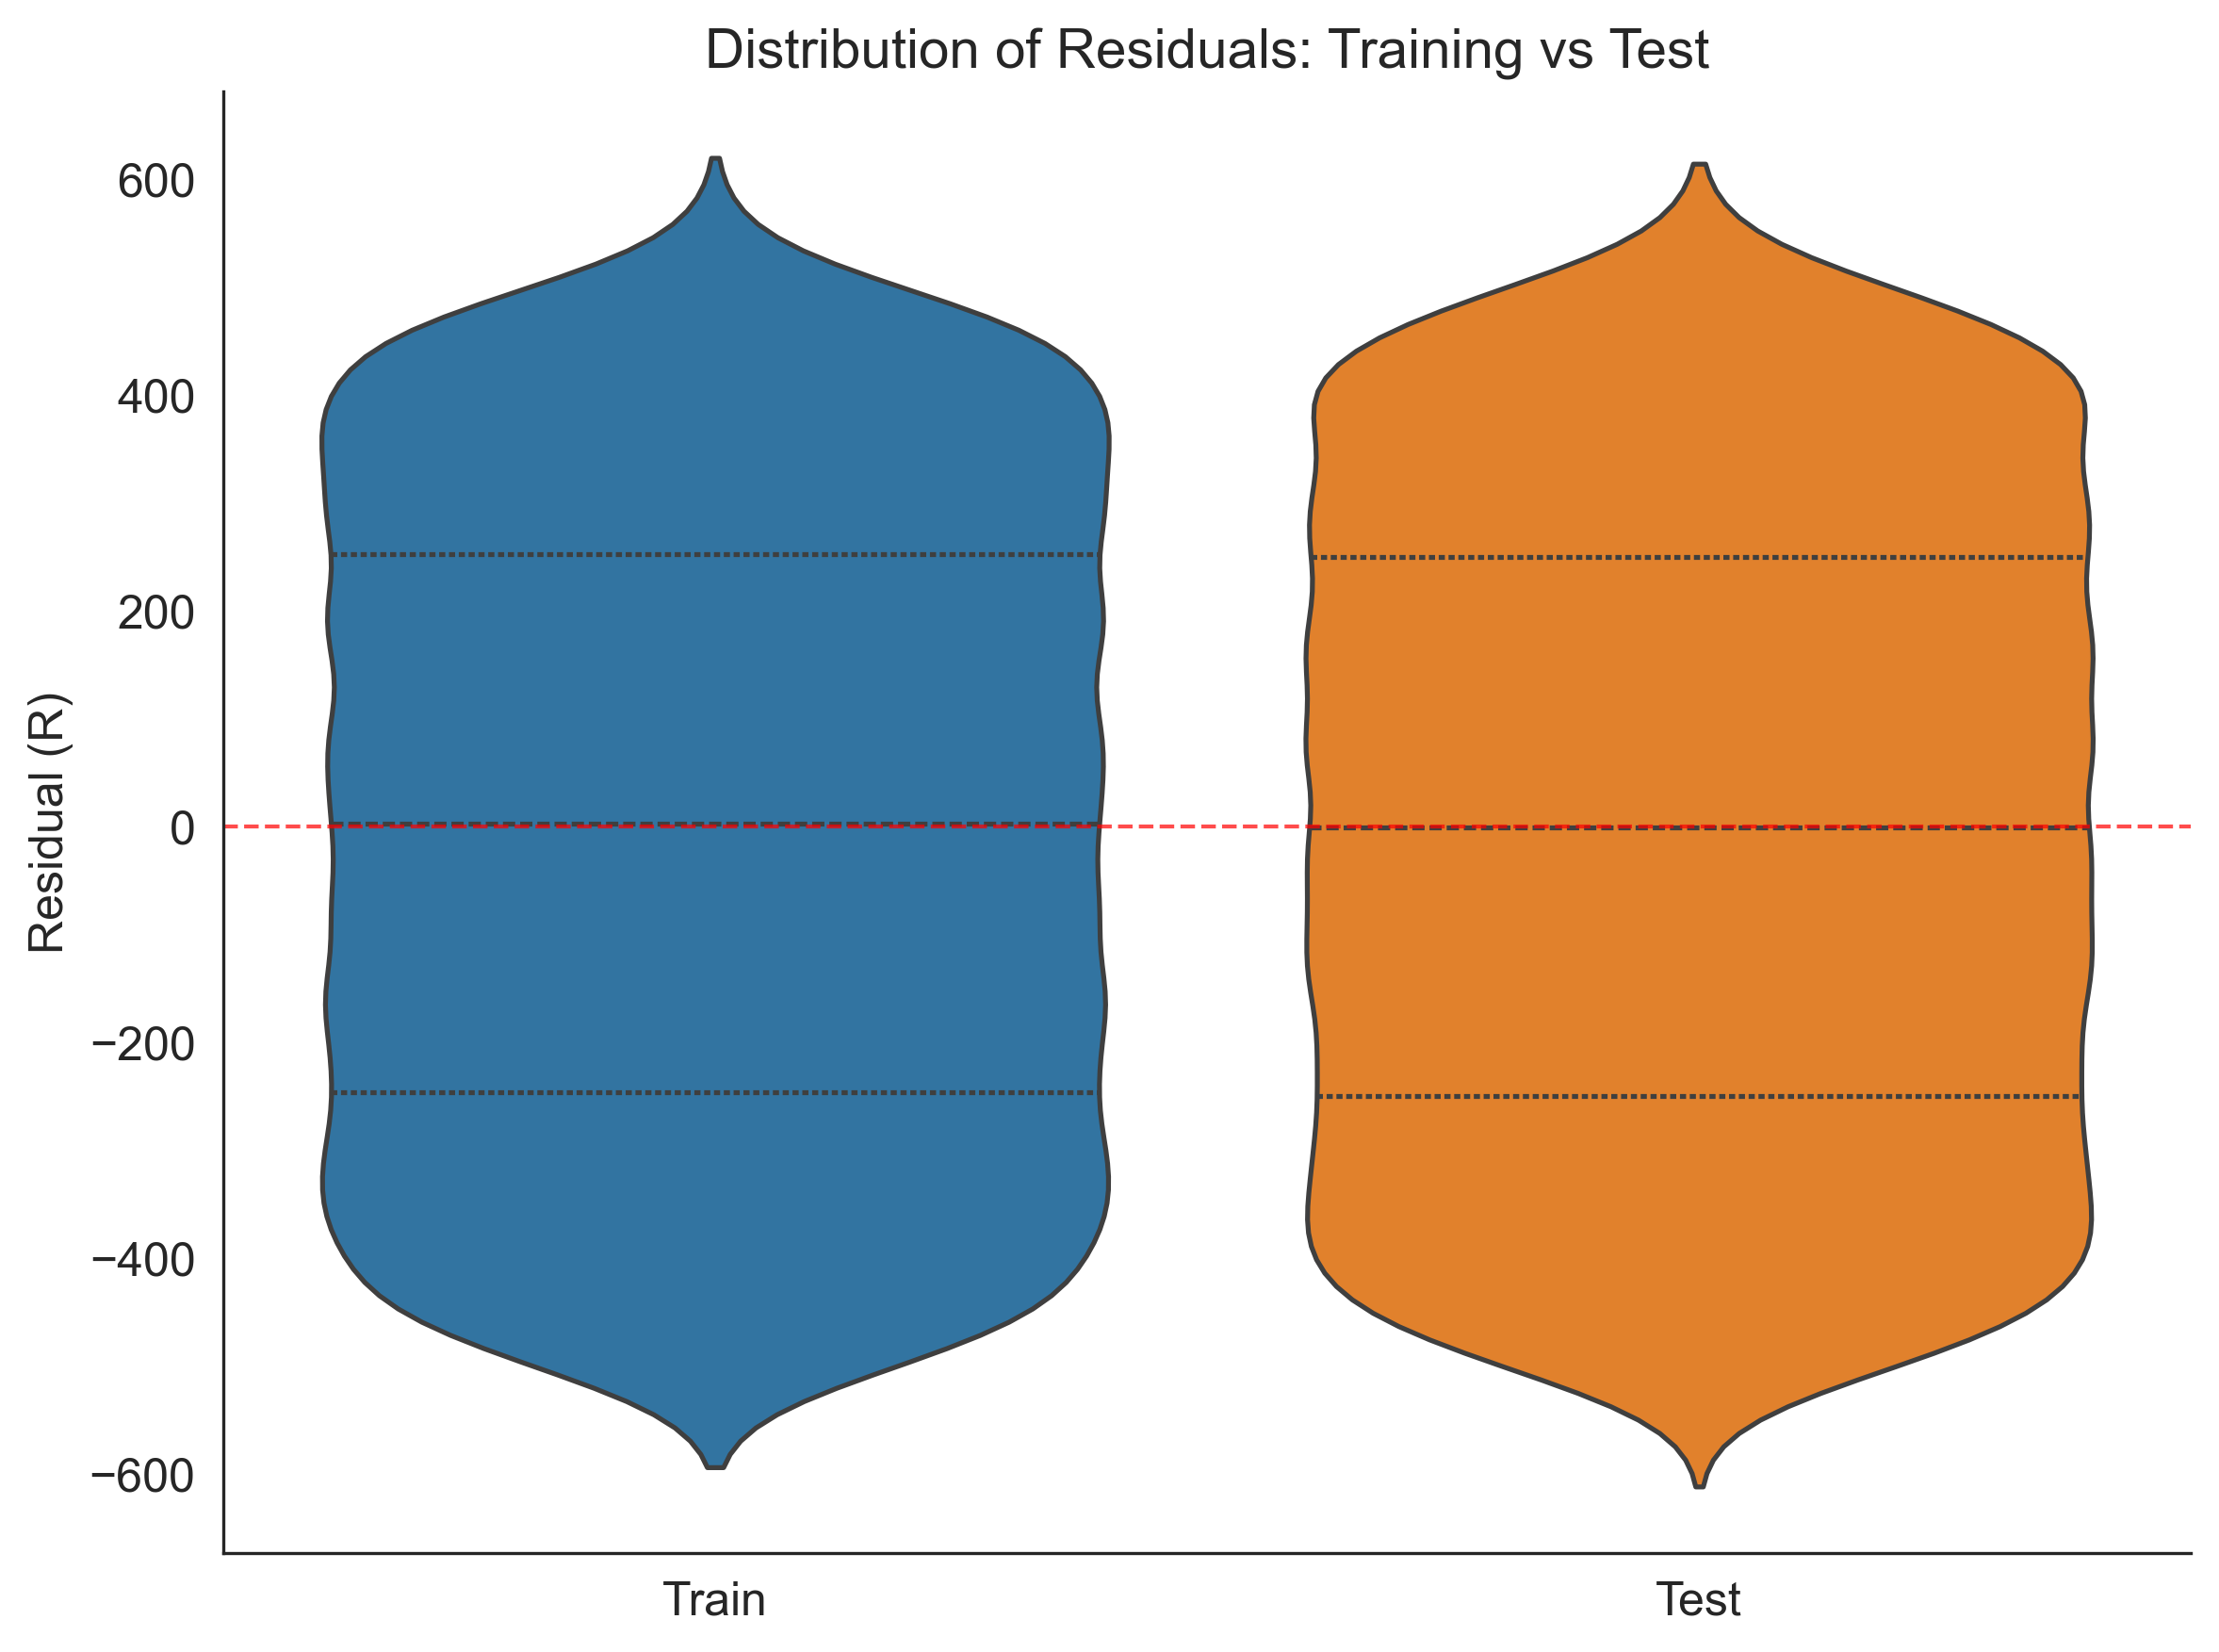
\includegraphics[width=\textwidth]{Thesis/Chapter 3/Figures/fig_violin_residuals.png}
    \caption{Violin plots of residuals on the training and test sets.}
    \label{fig:violin_residuals_ch3}
\end{subfigure}
\caption{Residual diagnostics for the fitted \gls{dnn}.}
\label{fig:residual_analysis_ch3}
\end{figure}

\noindent
Figure~\ref{fig:residual_diagnostics_ch3} presents the four residual
diagnostic panels for the test set. Panel~(a) shows residuals versus fitted
values: the residuals are centred at zero across the full range of fitted
charges (approximately R5\,000 to R30\,000), with no visible funnel shape
or systematic trend. The residual magnitudes range from approximately
$-600$ to $+600$, which is small relative to the response scale.
Panel~(b) displays the residual histogram, which is symmetric and centred
at zero but distinctly non-Gaussian: the distribution is platykurtic and
plateau-shaped, with probability spread nearly evenly across a bounded
interval and hard cutoffs near $\pm 600$ rather than smoothly decaying
tails. Panel~(c) shows the Q-Q plot of standardised residuals. The central
portion follows the theoretical reference line, while both tails bend
markedly away from it, confirming that the residual distribution is
bounded, with far lighter tails than a Gaussian distribution. This
bounded, near-uniform residual shape is the fingerprint of the benchmark's
data-generating process: the response is produced by a deterministic cost
formula with a bounded random perturbation, which explains both the hard
residual cutoffs and the near-ceiling $R^2$ values observed on every
partition. Consequently, the accuracy figures reported in this study
characterise how well the network recovers an algorithmic generating
formula, and no claim is made that these specific figures transfer to real
insurance portfolios (see the delimitations in
Section~\ref{sec:scope_delimitations}). The non-Gaussian residual shape is
not itself a concern for the \gls{dnn}, which does not assume normality of
residuals. Panel~(d) plots
residuals against observation index: the points are scattered randomly
around zero with no discernible sequential pattern.
Figure~\ref{fig:violin_residuals_ch3} compares the residual distributions
across partitions. Both the training and test violins are centred at zero
and are nearly identical in width, spread and symmetry, confirming that the
residual error does not systematically differ between the training and test
data and that the fitted \gls{dnn} does not overfit the training partition.

\subsubsection{Principal component structural diagnostics}
\label{sec:pca_structural_diagnostics}

\gls{pca} is employed as a structural diagnostic of the standardised,
model-ready input space.  It is not used for dimension reduction, and no
predictors are removed on the basis of the principal components.  The
purpose is twofold: to assess whether the data partition preserves the
structure of the input space, and to check whether the fitted predictions
reproduce the dominant target pattern when displayed on the same
low-dimensional projection.

Let
$\widetilde{\mathbf{X}} \in \mathbb{R}^{n_{\mathrm{train}} \times p}$
denote the column-standardised training input matrix ($p = 22$).  The
sample covariance matrix is
\begin{equation}
    \mathbf{S}
    = \frac{1}{n_{\mathrm{train}}-1}\,
      \widetilde{\mathbf{X}}^{\!\top}\widetilde{\mathbf{X}} .
    \label{eq:pca_covariance_matrix}
\end{equation}
\equationlistentry{PCA sample covariance matrix}
Its spectral decomposition is
\begin{equation}
    \mathbf{S}
    = \mathbf{W}\boldsymbol{\Lambda}\mathbf{W}^{\!\top},
    \qquad
    \boldsymbol{\Lambda}
    = \operatorname{diag}(\lambda_1,\dots,\lambda_p),
    \qquad
    \lambda_1 \geq \lambda_2 \geq \cdots \geq \lambda_p \geq 0 ,
    \label{eq:pca_eigendecomposition}
\end{equation}
\equationlistentry{PCA eigenvalue decomposition}
where $\mathbf{W} = [\mathbf{w}_1 \cdots \mathbf{w}_p]$ contains the
principal loading vectors.  The score of observation $i$ on component
$k$ is
\begin{equation}
    z_{ik} = \widetilde{\mathbf{x}}_i^{\!\top}\mathbf{w}_k,
    \qquad k = 1,\dots,p .
    \label{eq:pca_scores}
\end{equation}
\equationlistentry{PCA principal component scores}
The \gls{pca} decomposition is computed from the training partition only; the
resulting eigenvectors are then used to project the validation and test
observations, so that all sets are displayed in a common coordinate system.
The first two principal components provide the two-dimensional diagnostic
projection.

Two \gls{pca} comparisons are performed.  First, the training, validation and test
point clouds are overlaid; similar structure across partitions supports the
view that the data split has not introduced a major structural shift.
Second, the same \gls{pca} coordinates are coloured by observed charges and by
fitted predictions; similar colour gradients indicate that the fitted
\gls{dnn} has captured the dominant target structure visible in the input
space.

The loading vectors are inspected to verify that the first two principal
components are not driven by a single variable and that they account for a
moderate share of the total variance, so that the diagnostic is not
dominated by one narrow direction \citep{hastie2009elements}.  This
inspection is descriptive and is not used to modify the fitted model.

\begin{figure}[H]
\centering
\begin{subfigure}[b]{0.48\textwidth}
    \centering
    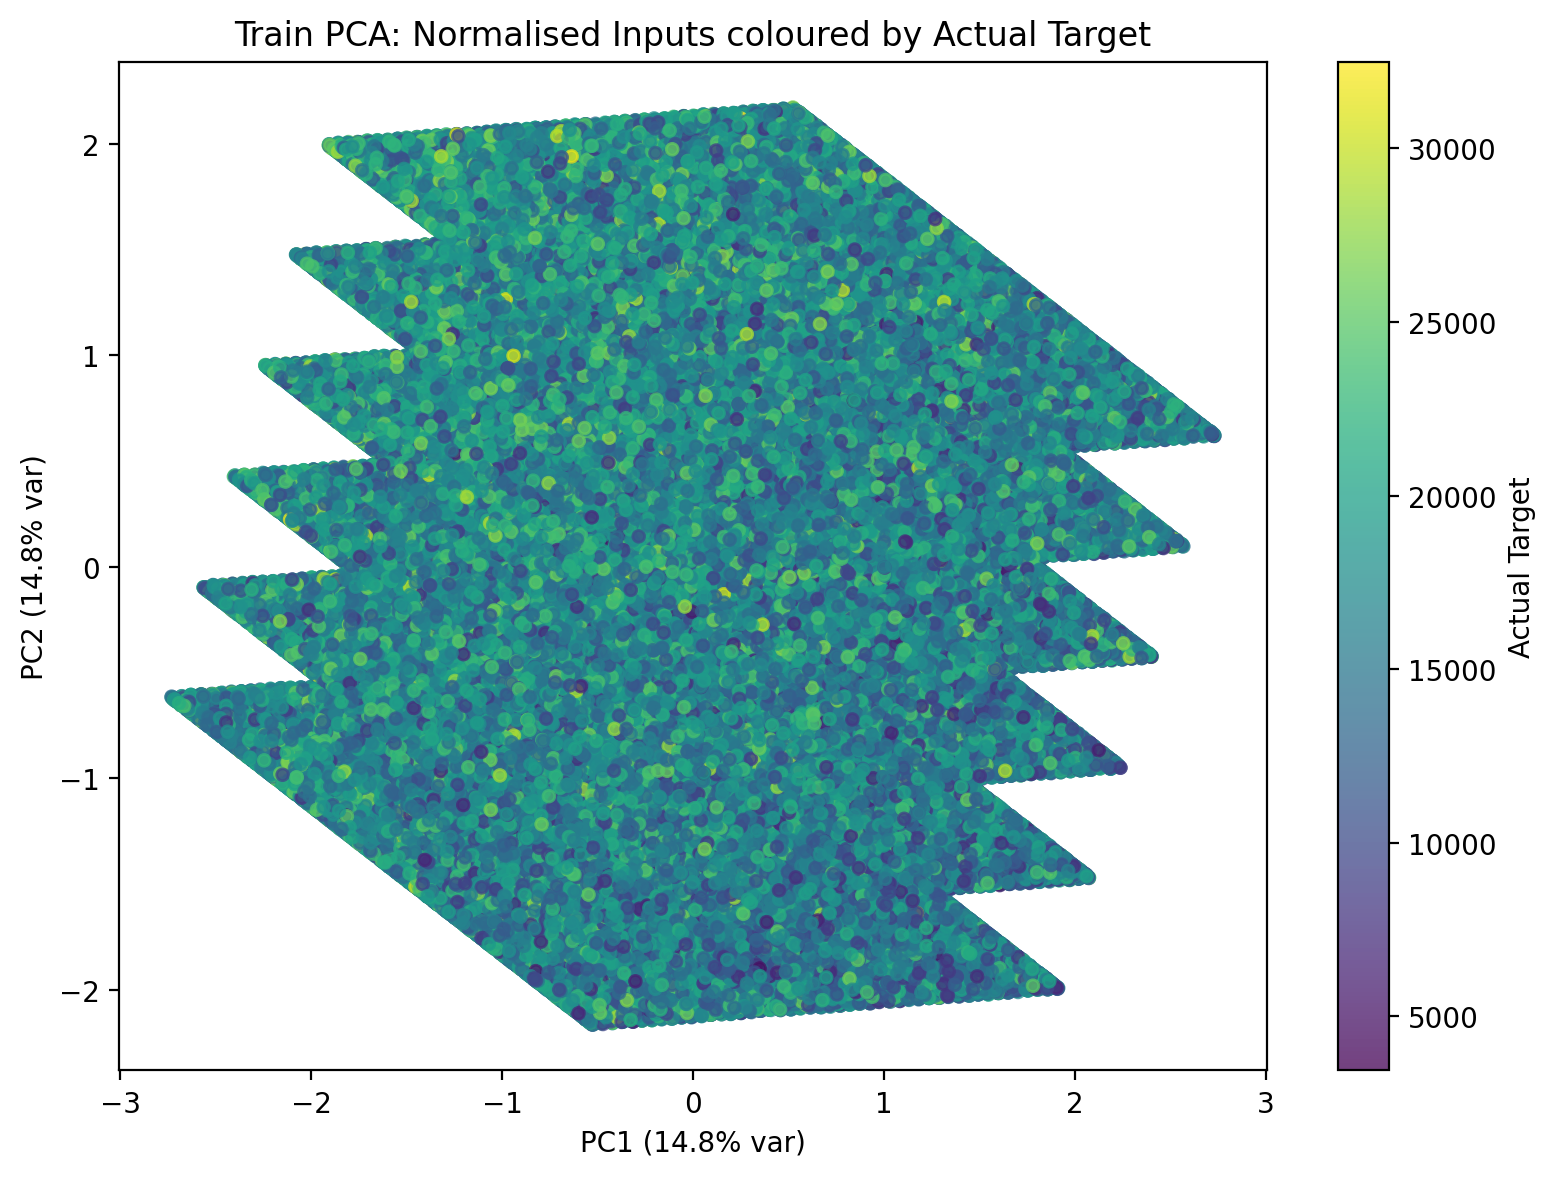
\includegraphics[width=\textwidth]{Thesis/Chapter 3/Figures/fig_sml_pca_train_actual.png}
    \caption{Training set, actual charges.}
    \label{fig:pca_train_actual_ch3}
\end{subfigure}
\hfill
\begin{subfigure}[b]{0.48\textwidth}
    \centering
    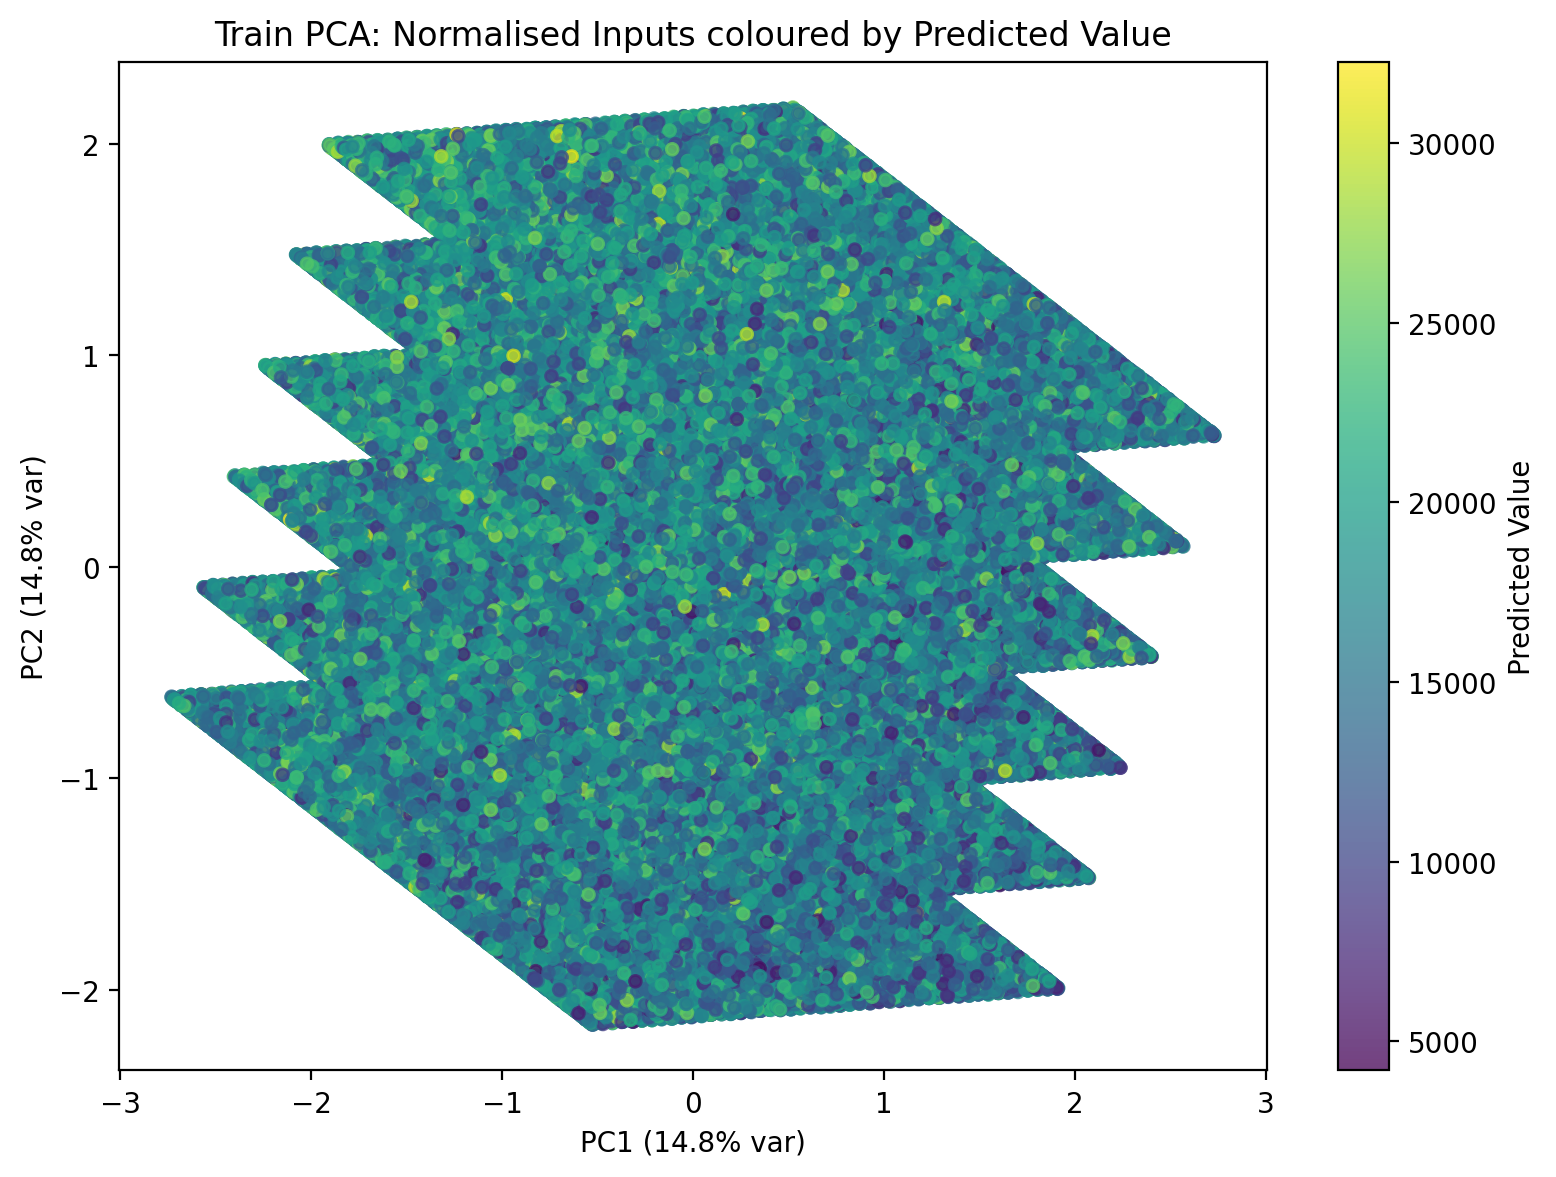
\includegraphics[width=\textwidth]{Thesis/Chapter 3/Figures/fig_sml_pca_train_predicted.png}
    \caption{Training set, predicted charges.}
    \label{fig:pca_train_predicted_ch3}
\end{subfigure}

\vspace{0.4cm}

\begin{subfigure}[b]{0.48\textwidth}
    \centering
    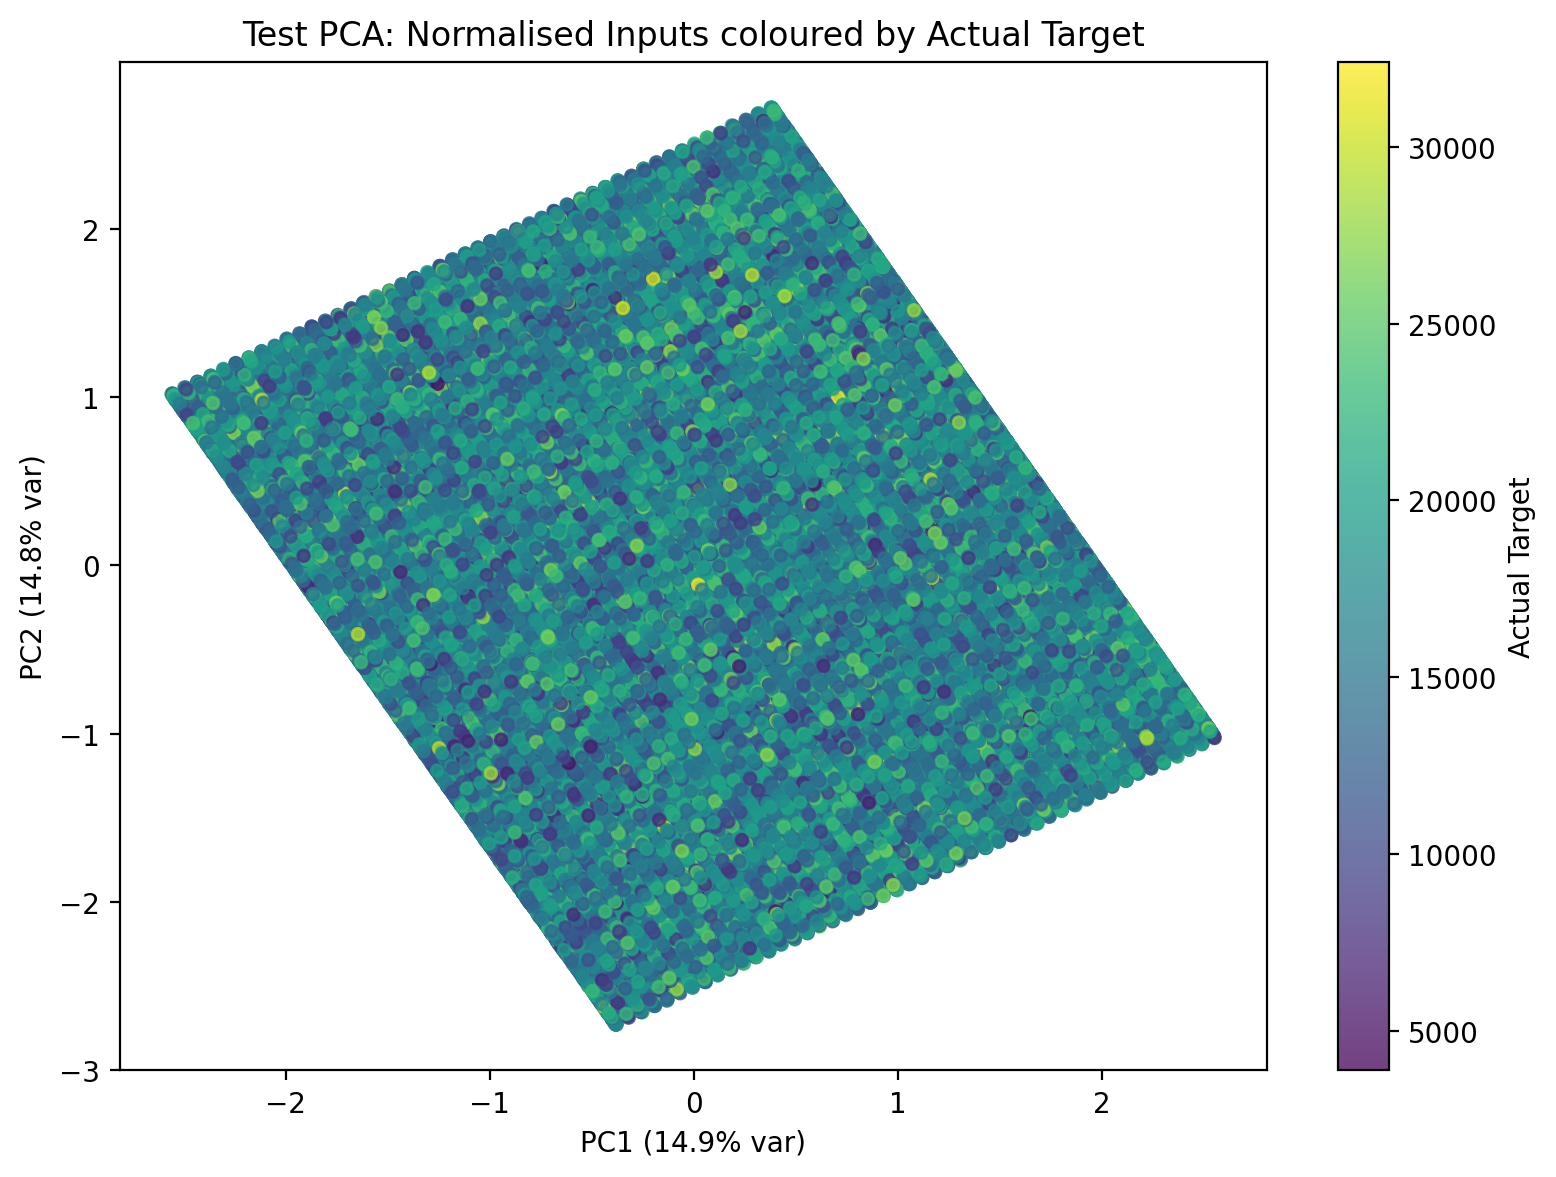
\includegraphics[width=\textwidth]{Thesis/Chapter 3/Figures/fig_sml_pca_test_actual.png}
    \caption{Test set, actual charges.}
    \label{fig:pca_test_actual_ch3}
\end{subfigure}
\hfill
\begin{subfigure}[b]{0.48\textwidth}
    \centering
    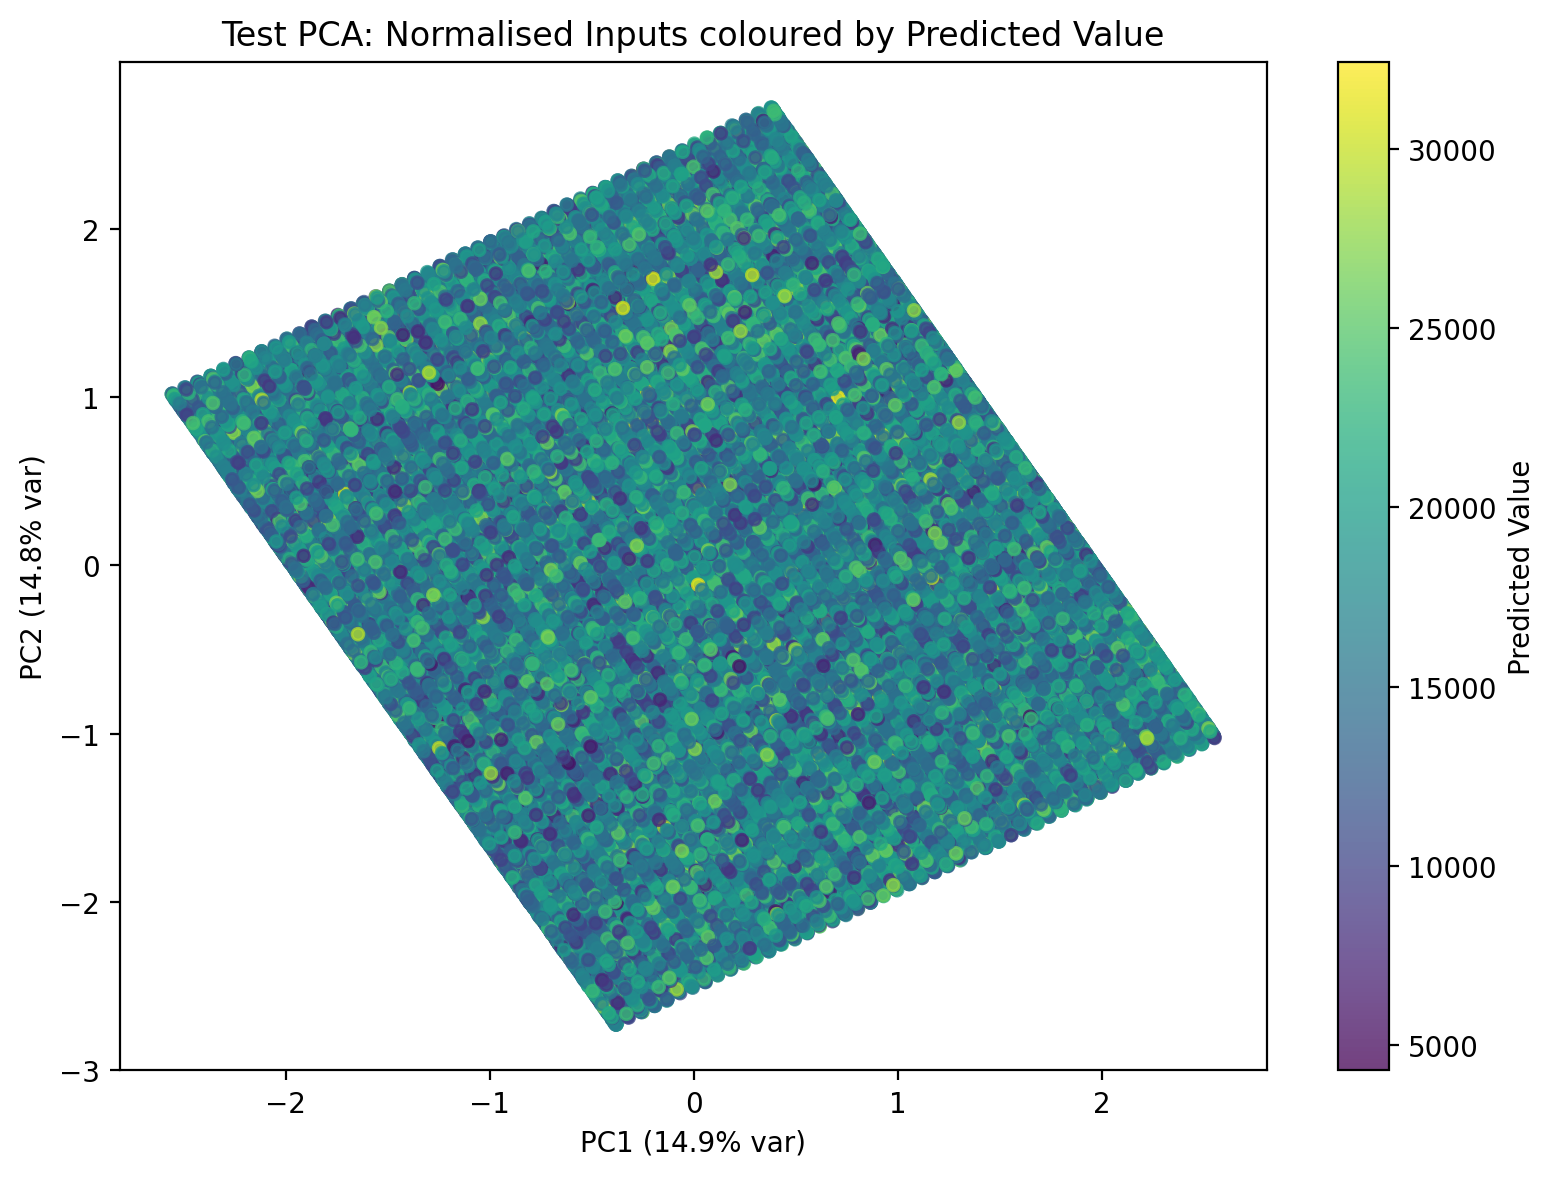
\includegraphics[width=\textwidth]{Thesis/Chapter 3/Figures/fig_sml_pca_test_predicted.png}
    \caption{Test set, predicted charges.}
    \label{fig:pca_test_predicted_ch3}
\end{subfigure}
\caption{\Gls{pca} projections coloured by actual and predicted charges on training and test sets.}
\label{fig:pca_diagnostics_ch3}
\end{figure}

\noindent
Figure~\ref{fig:pca_diagnostics_ch3} displays the \gls{pca} diagnostic scatter
plots. In the training set
(Figures~\ref{fig:pca_train_actual_ch3}
and~\ref{fig:pca_train_predicted_ch3}), the first two principal components
each explain approximately 14.8\% of the total variance. The point cloud
exhibits a layered structure with several horizontal shelves, reflecting the
discrete levels of the encoded categorical predictors projected onto the PC
axes. The colour gradient, representing charges from approximately R5\,000
(purple) to R30\,000 (yellow), is broadly mixed across the point cloud,
with higher charges (yellow-green) tending to appear at specific regions
within the layered structure. The predicted-target colouring
(Figure~\ref{fig:pca_train_predicted_ch3}) is virtually indistinguishable
from the actual-target version, confirming that the fitted \gls{dnn} has captured
the dominant target structure visible in the first two principal component
directions. The test set
(Figures~\ref{fig:pca_test_actual_ch3}
and~\ref{fig:pca_test_predicted_ch3}) shows the same point-cloud shape and
colour distribution as the training set (PC1: 14.9\%, PC2: 14.8\%),
and the actual and predicted colourings again match closely. This
consistency across partitions and between actual and predicted targets
jointly satisfies both the partition consistency and model capture
diagnostic criteria.

\begin{figure}[H]
\centering
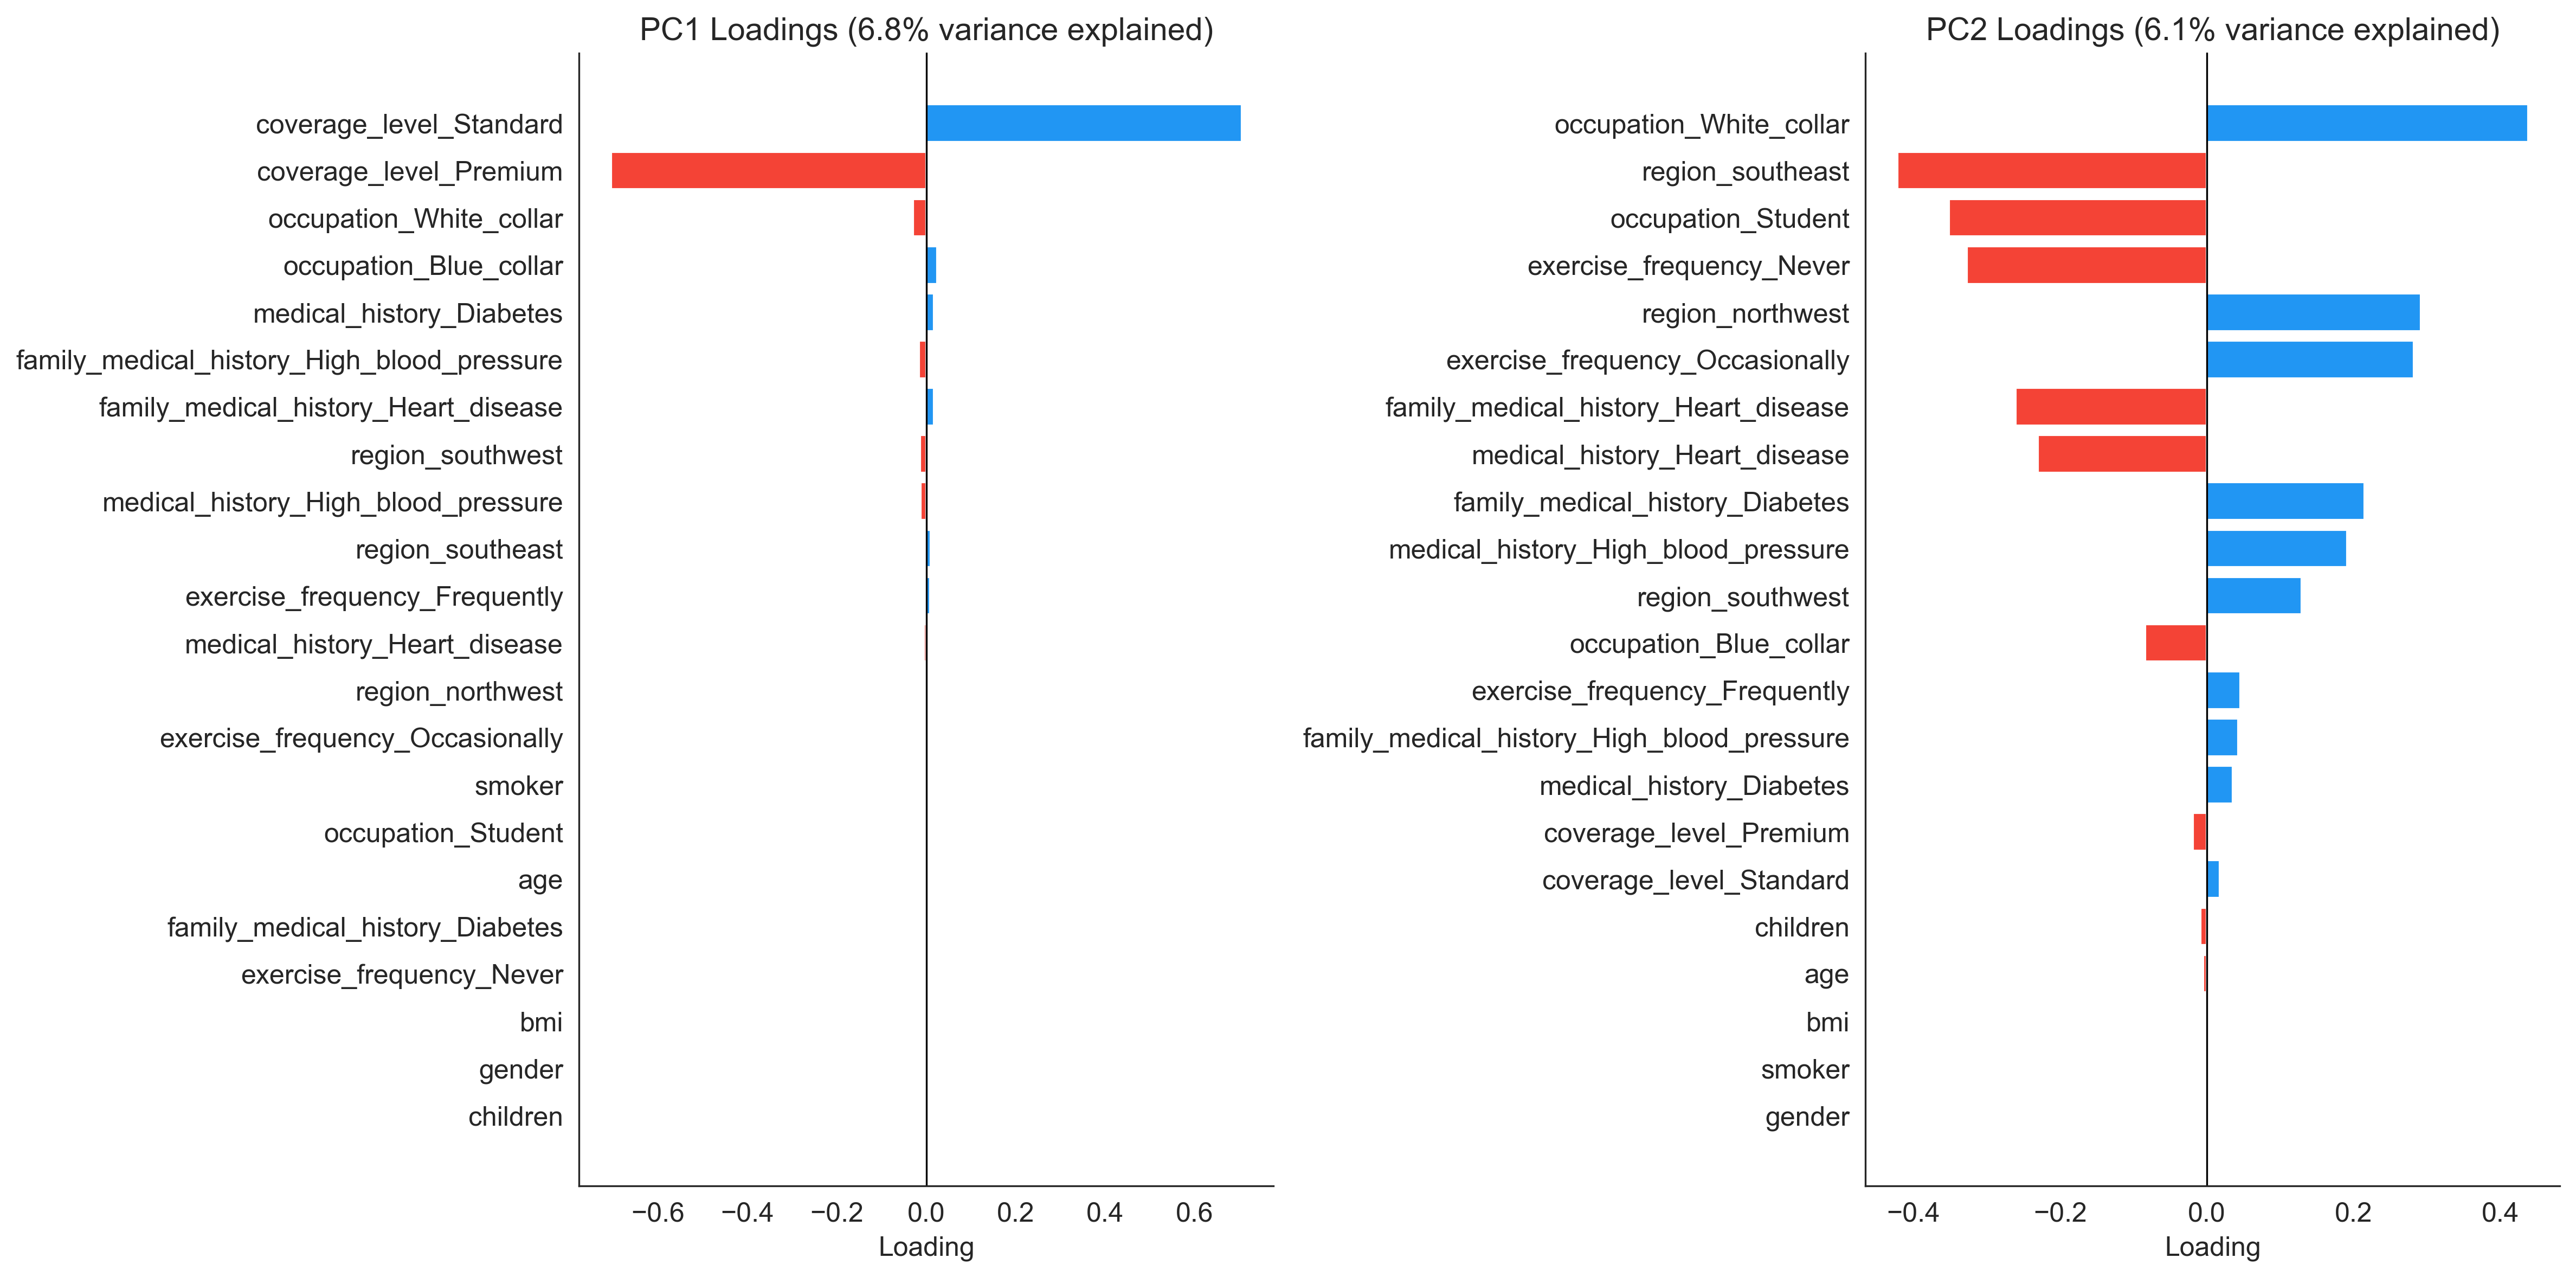
\includegraphics[width=0.90\textwidth]{Thesis/Chapter 3/Figures/fig_pca_loadings.png}
\caption{\Gls{pca} loading vectors for all 22 encoded predictors.}
\label{fig:pca_loadings_ch3}
\end{figure}

\noindent
Figure~\ref{fig:pca_loadings_ch3} displays the loading vectors for the
first two principal components. In the left panel, PC1 (6.8\% of
variance) is dominated by \texttt{coverage\_level\_\allowbreak{}Standard} (positive
loading $\approx 0.71$) and \texttt{coverage\_level\_\allowbreak{}Premium} (negative
loading $\approx -0.71$), with all other loadings substantially smaller in
magnitude. This confirms that the layered structure observed in the
scatter plots is driven by the \texttt{coverage\_\allowbreak{}level} variable. In the
right panel, PC2 (6.1\% of variance) has loadings spread across multiple
categorical predictors: \texttt{occupation\_\allowbreak{}White\_collar} ($\approx 0.44$),
\texttt{region\_\allowbreak{}northwest} ($\approx 0.33$) and
\texttt{exercise\_frequency\_\allowbreak{}Never} ($\approx 0.30$) contribute positively,
while \texttt{region\_\allowbreak{}southeast} ($\approx -0.42$) and
\texttt{medical\_history\_\allowbreak{}Heart\_disease} ($\approx -0.20$) contribute
negatively. The more distributed loading structure of PC2 indicates that no
single variable dominates the second component. Although PC1 is driven by a
single raw variable, the first two components together account for only
13\% of total variance, so the diagnostic is not determined by a single
narrow direction in the 22-dimensional input space.

\subsubsection{Correlation heatmap diagnostics}
\label{sec:correlation_heatmap_diagnostics}

Correlation heatmaps provide an additional structural check.  The full
Pearson correlation matrix is computed for the standardised encoded
predictors together with either the observed response or the fitted
predictions, yielding two views:
\begin{enumerate}
    \item correlations between predictors and observed charges;
    \item correlations between predictors and fitted predictions.
\end{enumerate}
Comparing these views indicates whether the fitted \gls{dnn} has preserved
the main linear feature-target relationships present in the data.  The
heatmaps are also produced for the training, validation and test partitions
to assess whether the data split preserves the linear dependence structure
of the model-ready input space.  These heatmaps are purely diagnostic; they
do not capture the nonlinear relationships learned by the network, nor do
they constitute a proof of model correctness.

\begin{figure}[H]
\centering
\begin{subfigure}[b]{0.48\textwidth}
    \centering
    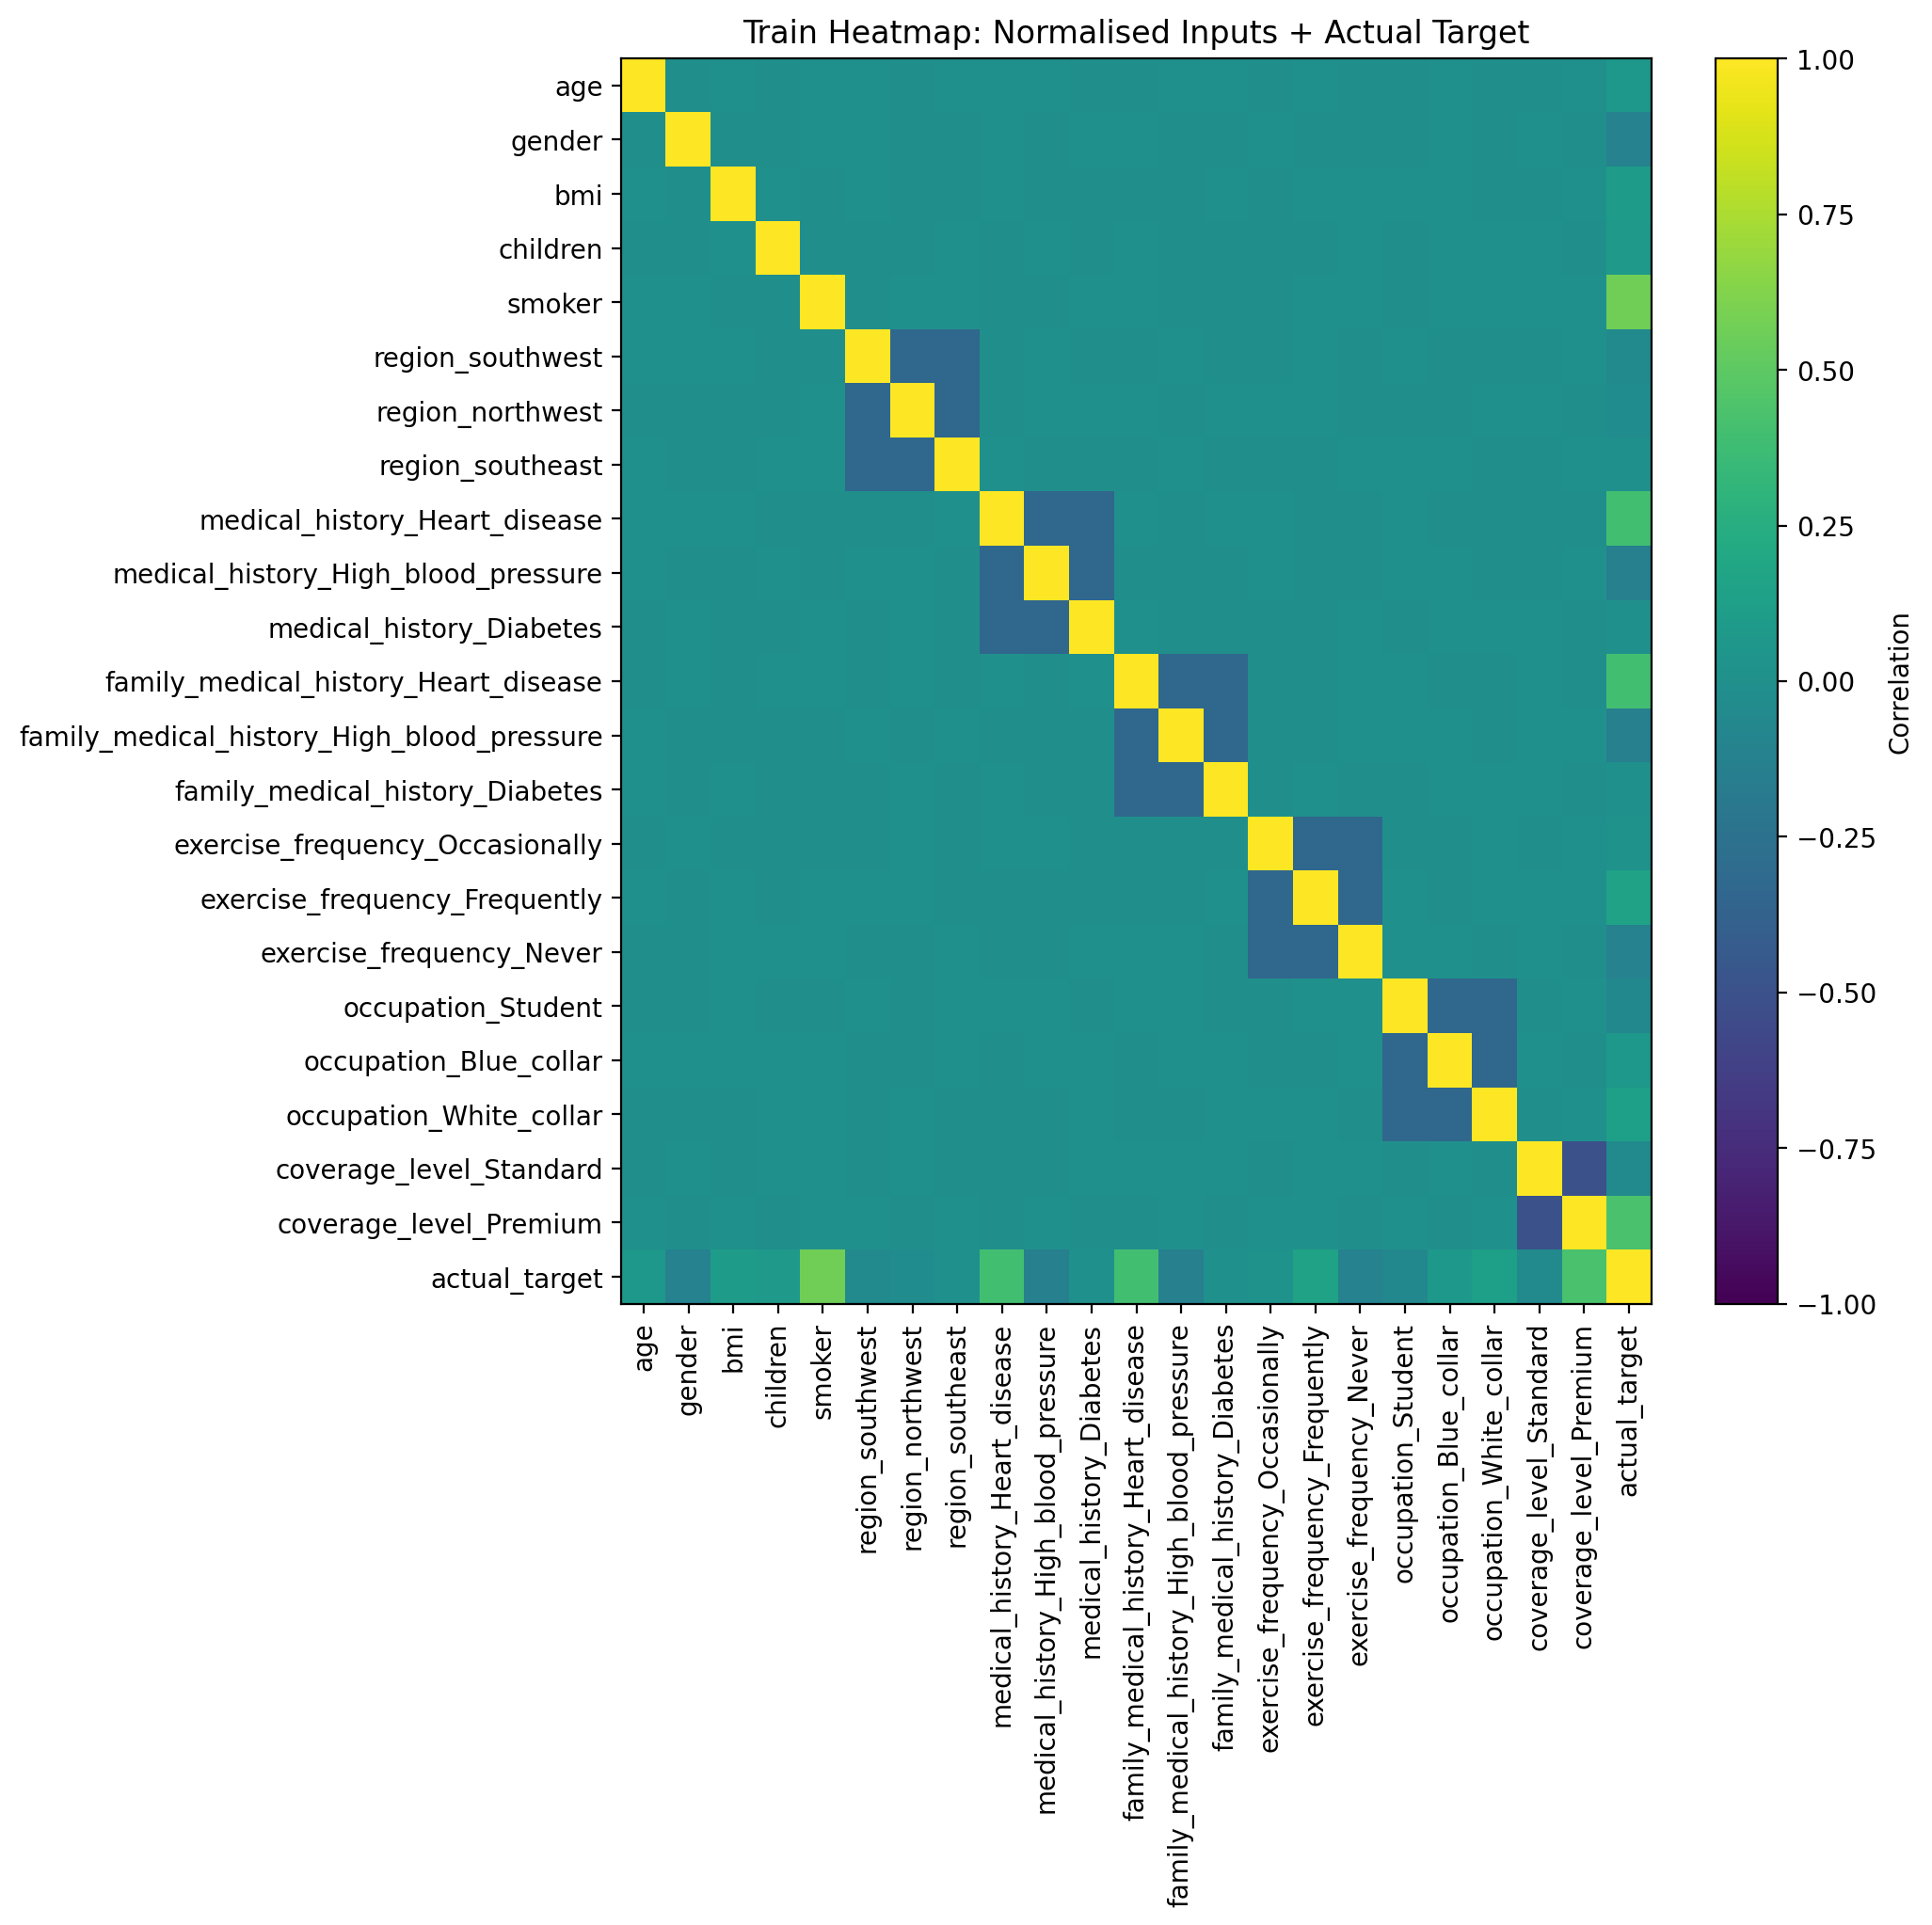
\includegraphics[width=\textwidth]{Thesis/Chapter 3/Figures/fig_sml_heatmap_train_actual.png}
    \caption{Training set, actual charges.}
    \label{fig:heatmap_train_actual_ch3}
\end{subfigure}
\hfill
\begin{subfigure}[b]{0.48\textwidth}
    \centering
    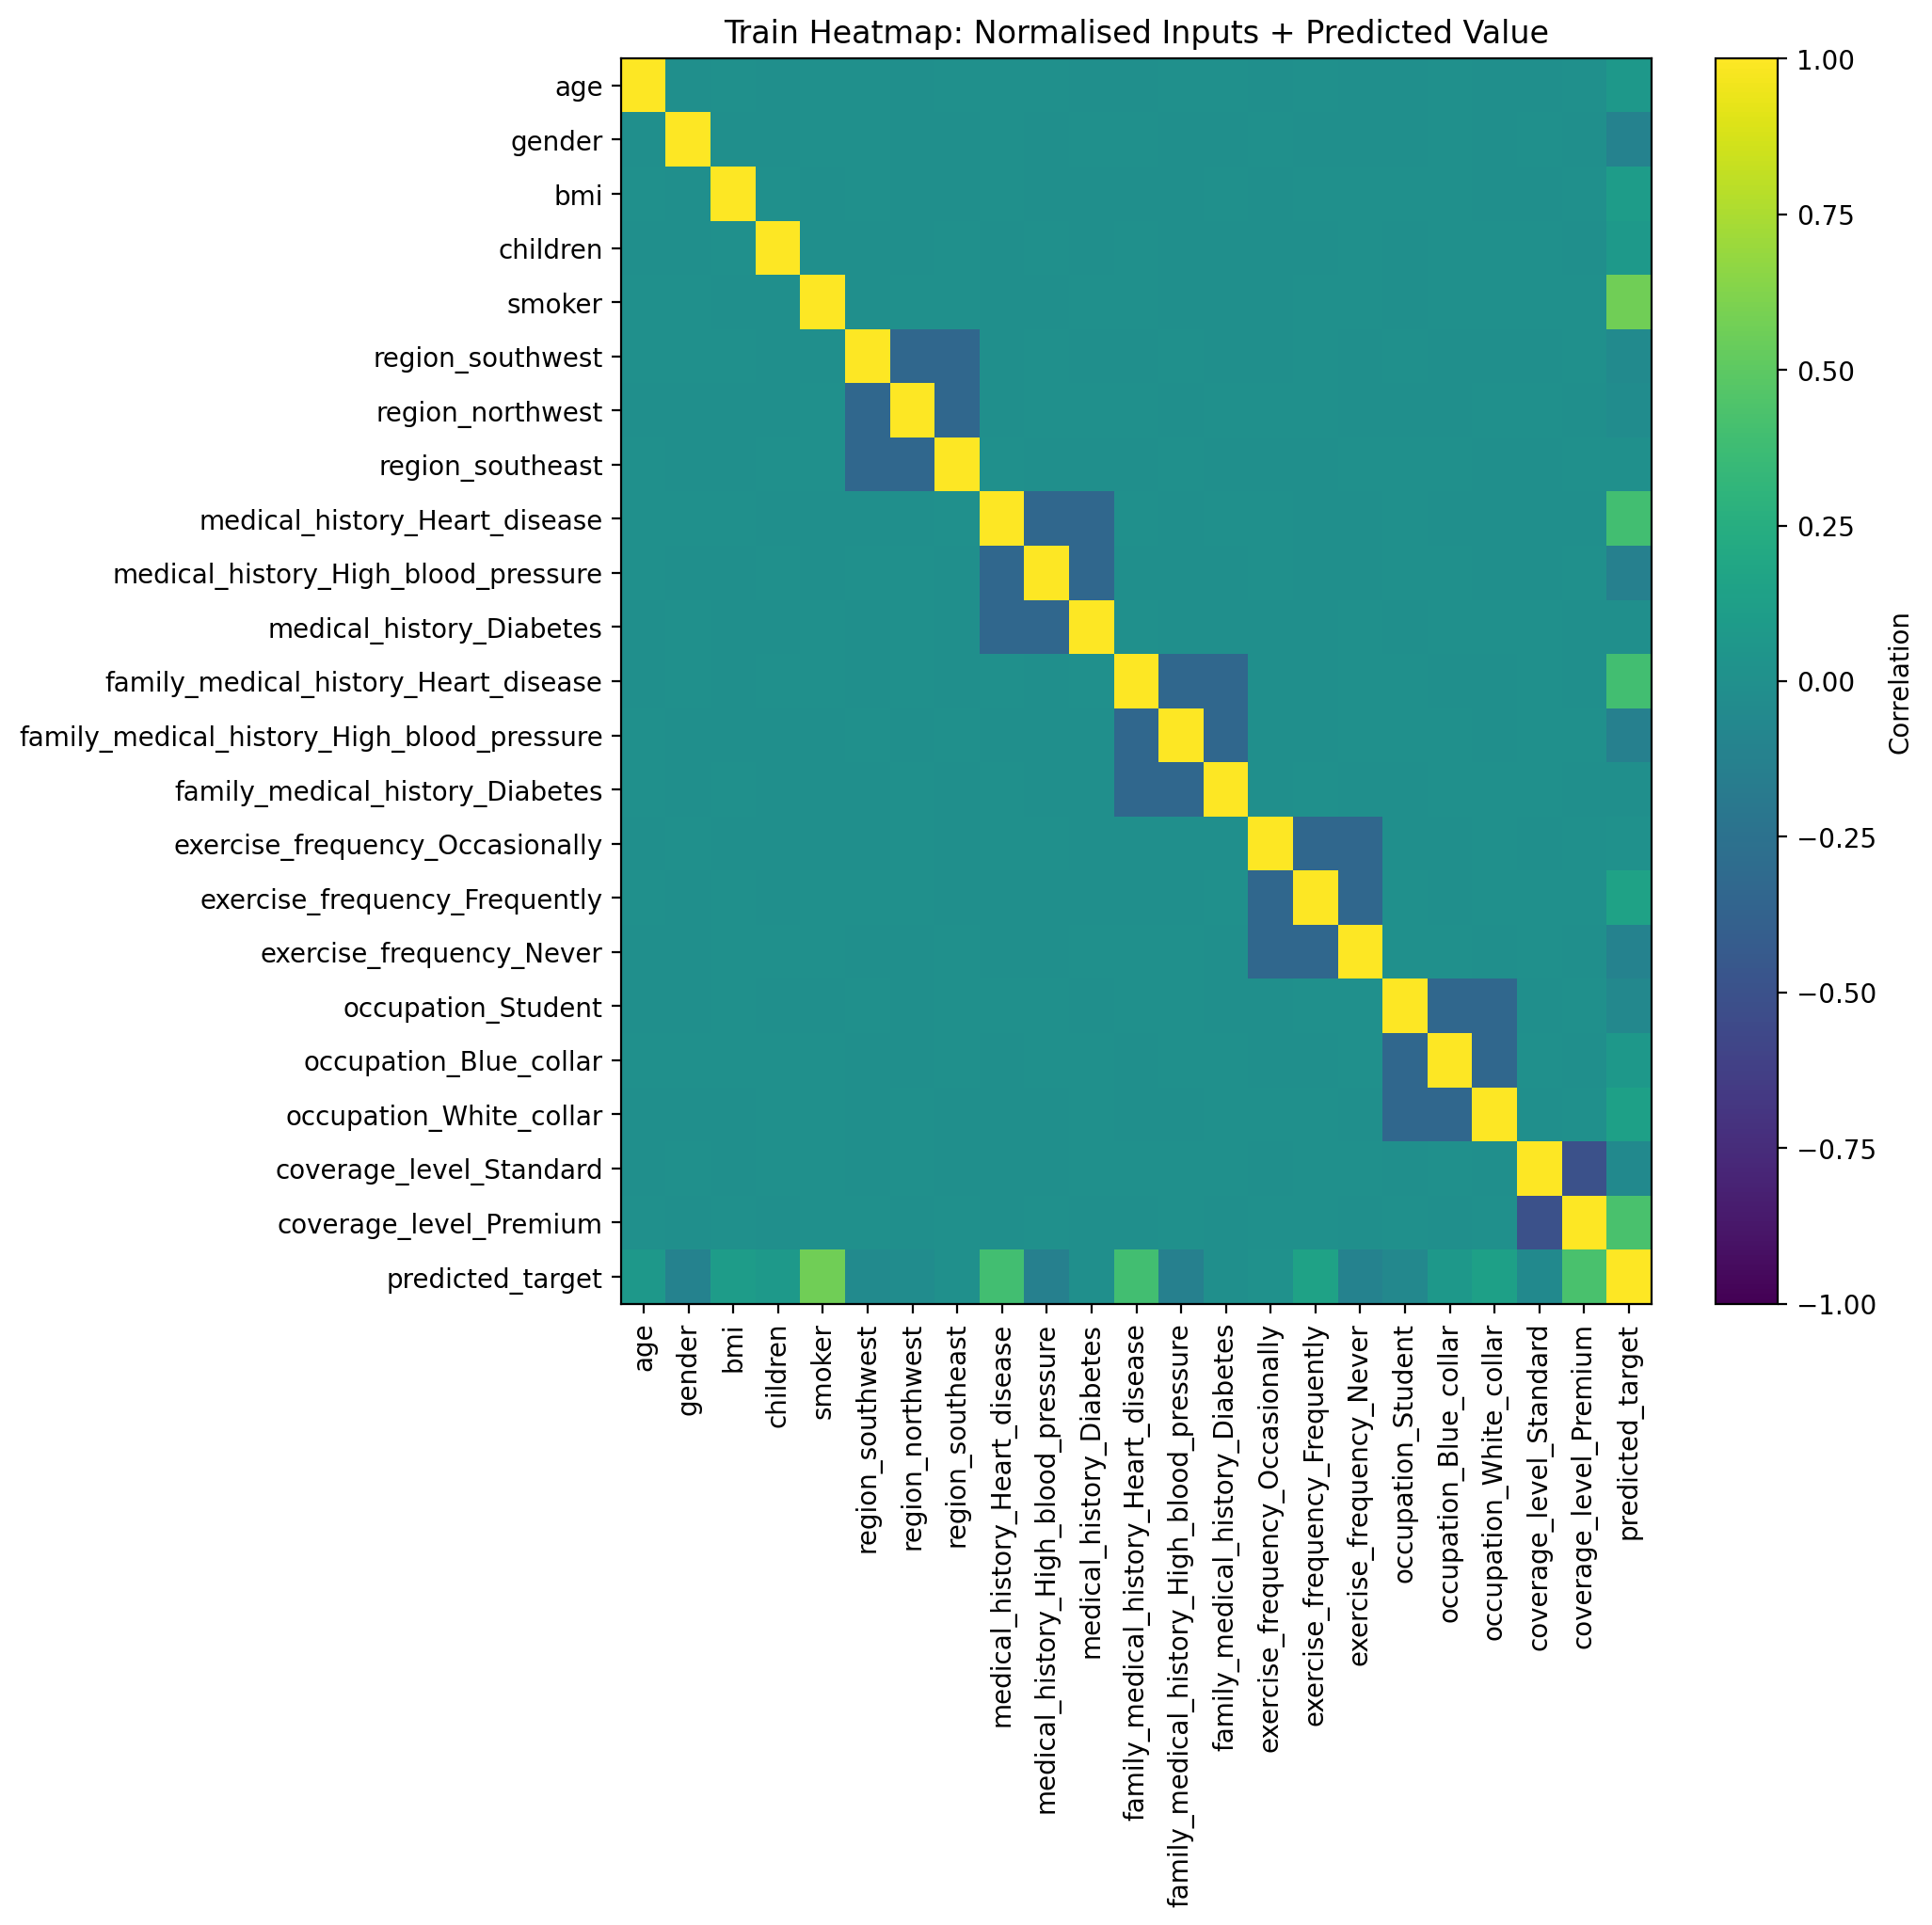
\includegraphics[width=\textwidth]{Thesis/Chapter 3/Figures/fig_sml_heatmap_train_predicted.png}
    \caption{Training set, predicted charges.}
    \label{fig:heatmap_train_predicted_ch3}
\end{subfigure}

\vspace{0.4cm}

\begin{subfigure}[b]{0.48\textwidth}
    \centering
    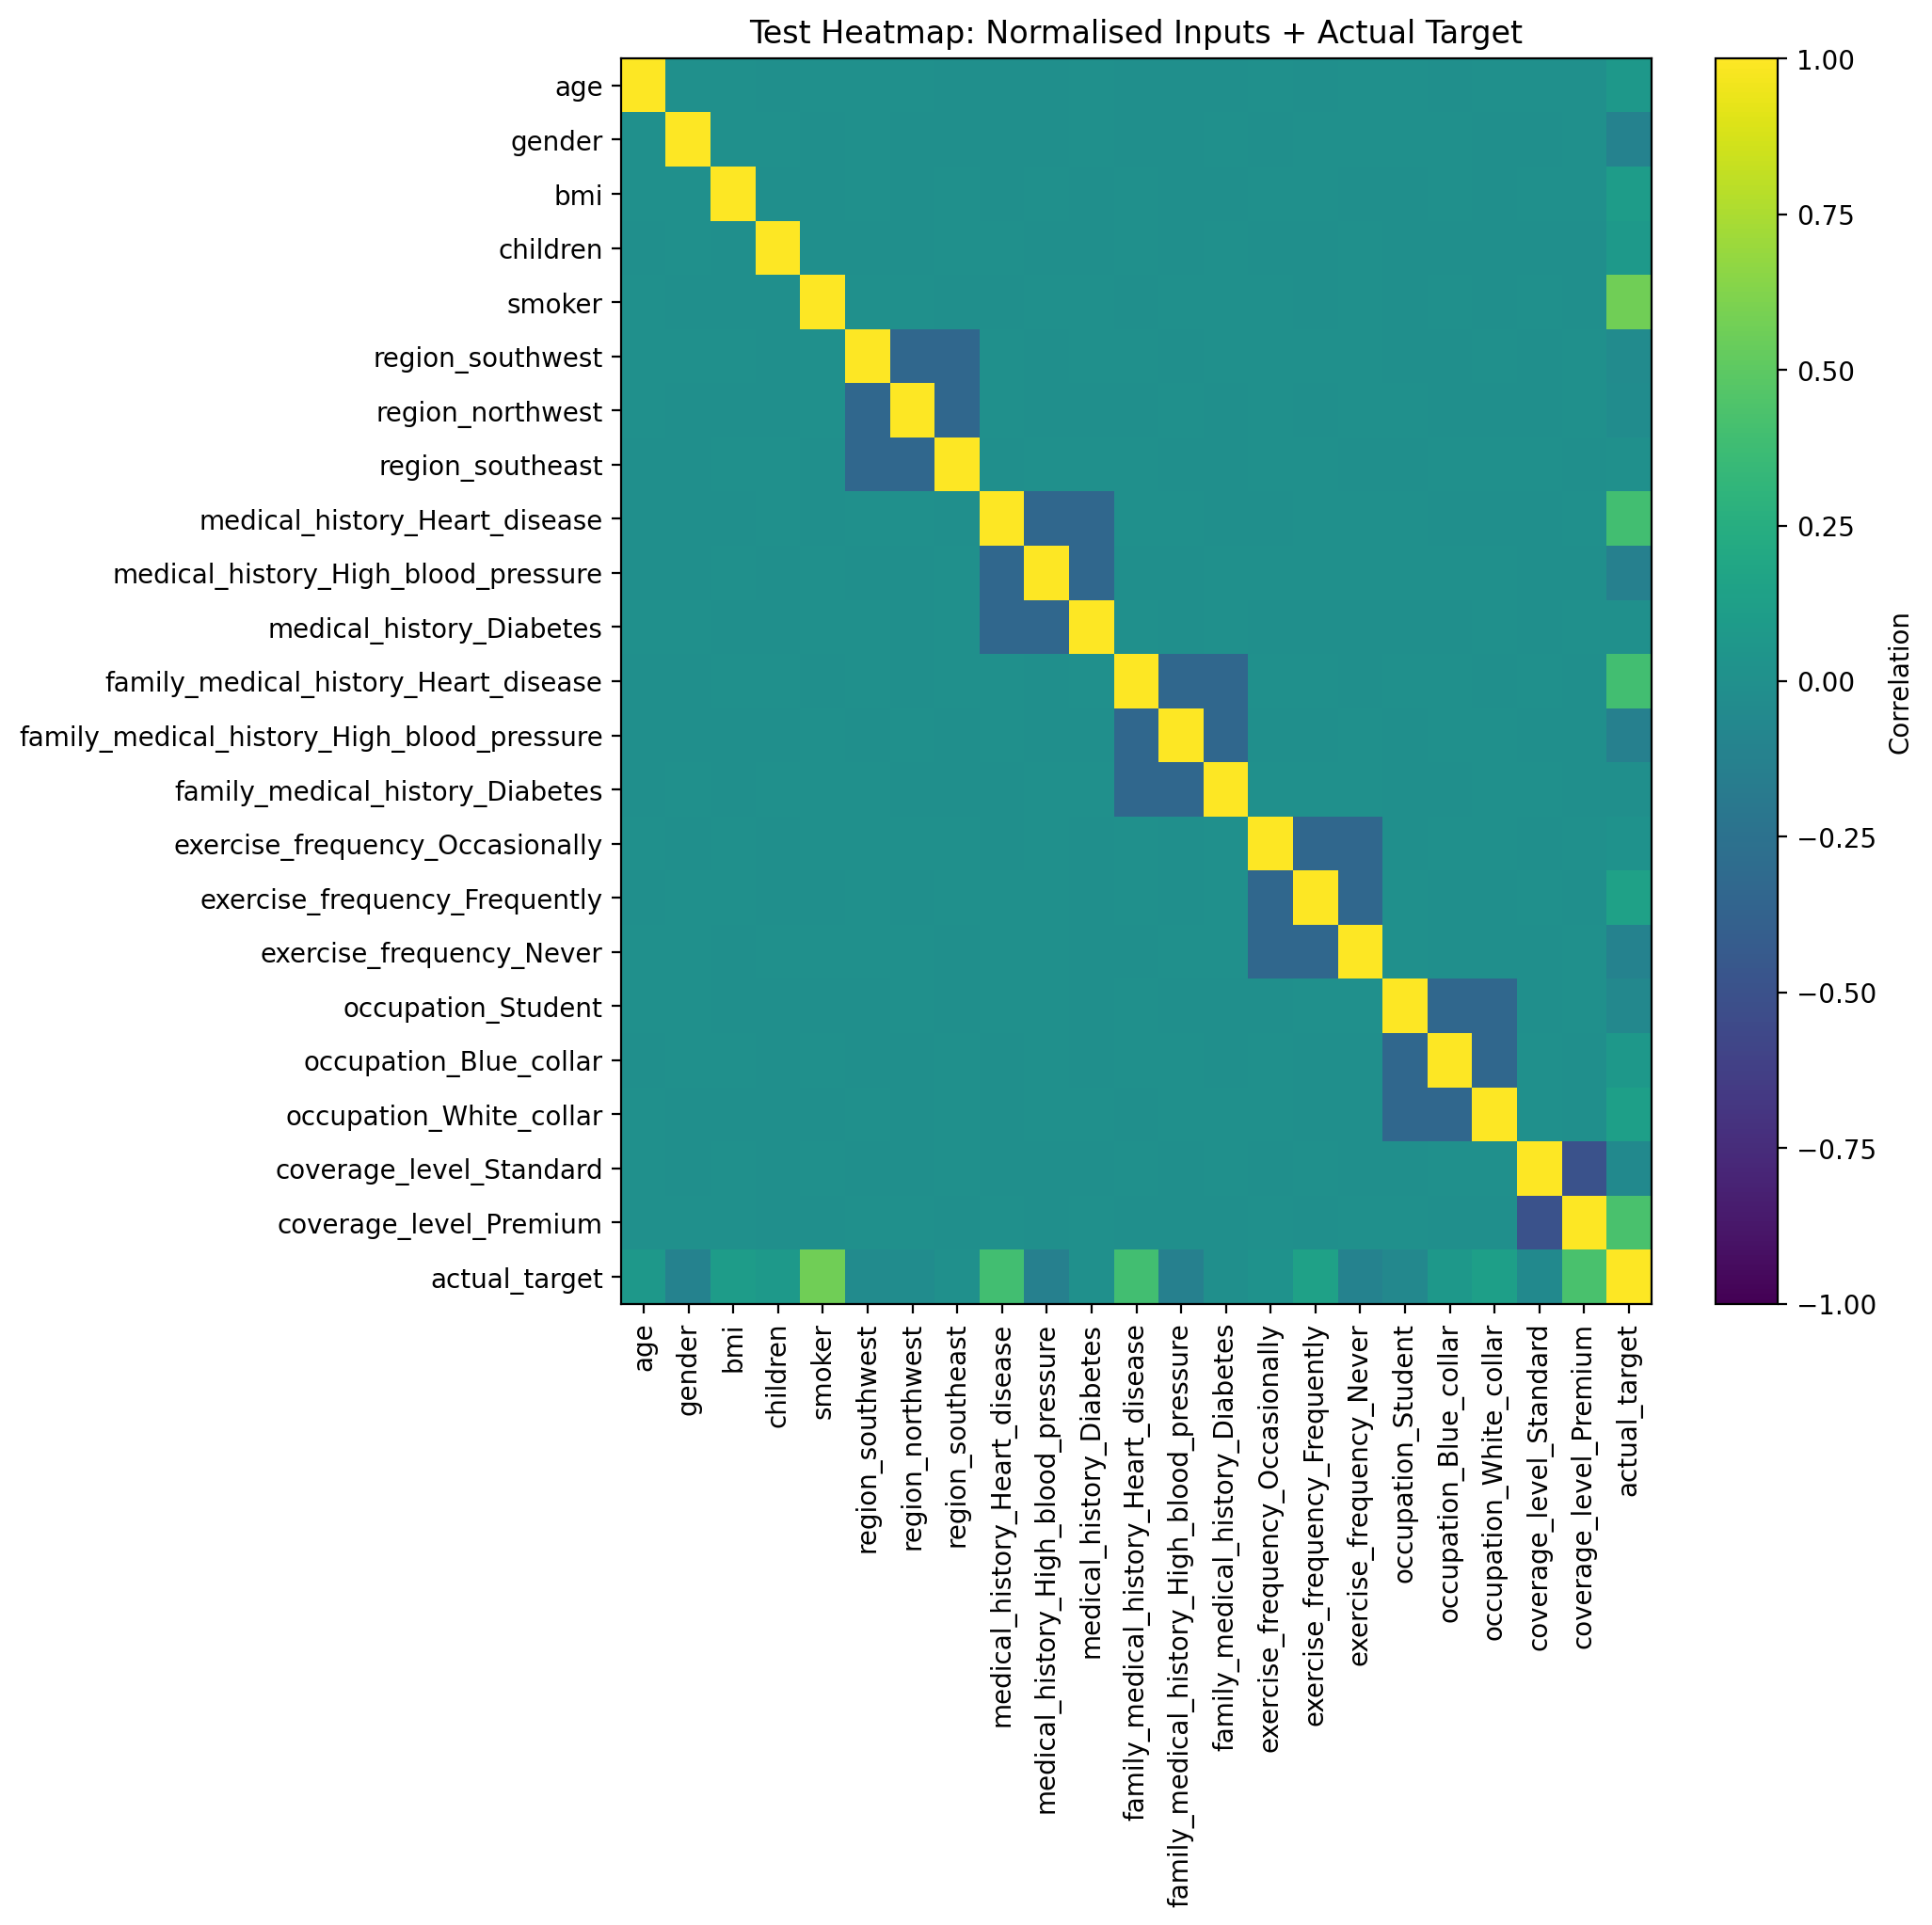
\includegraphics[width=\textwidth]{Thesis/Chapter 3/Figures/fig_sml_heatmap_test_actual.png}
    \caption{Test set, actual charges.}
    \label{fig:heatmap_test_actual_ch3}
\end{subfigure}
\hfill
\begin{subfigure}[b]{0.48\textwidth}
    \centering
    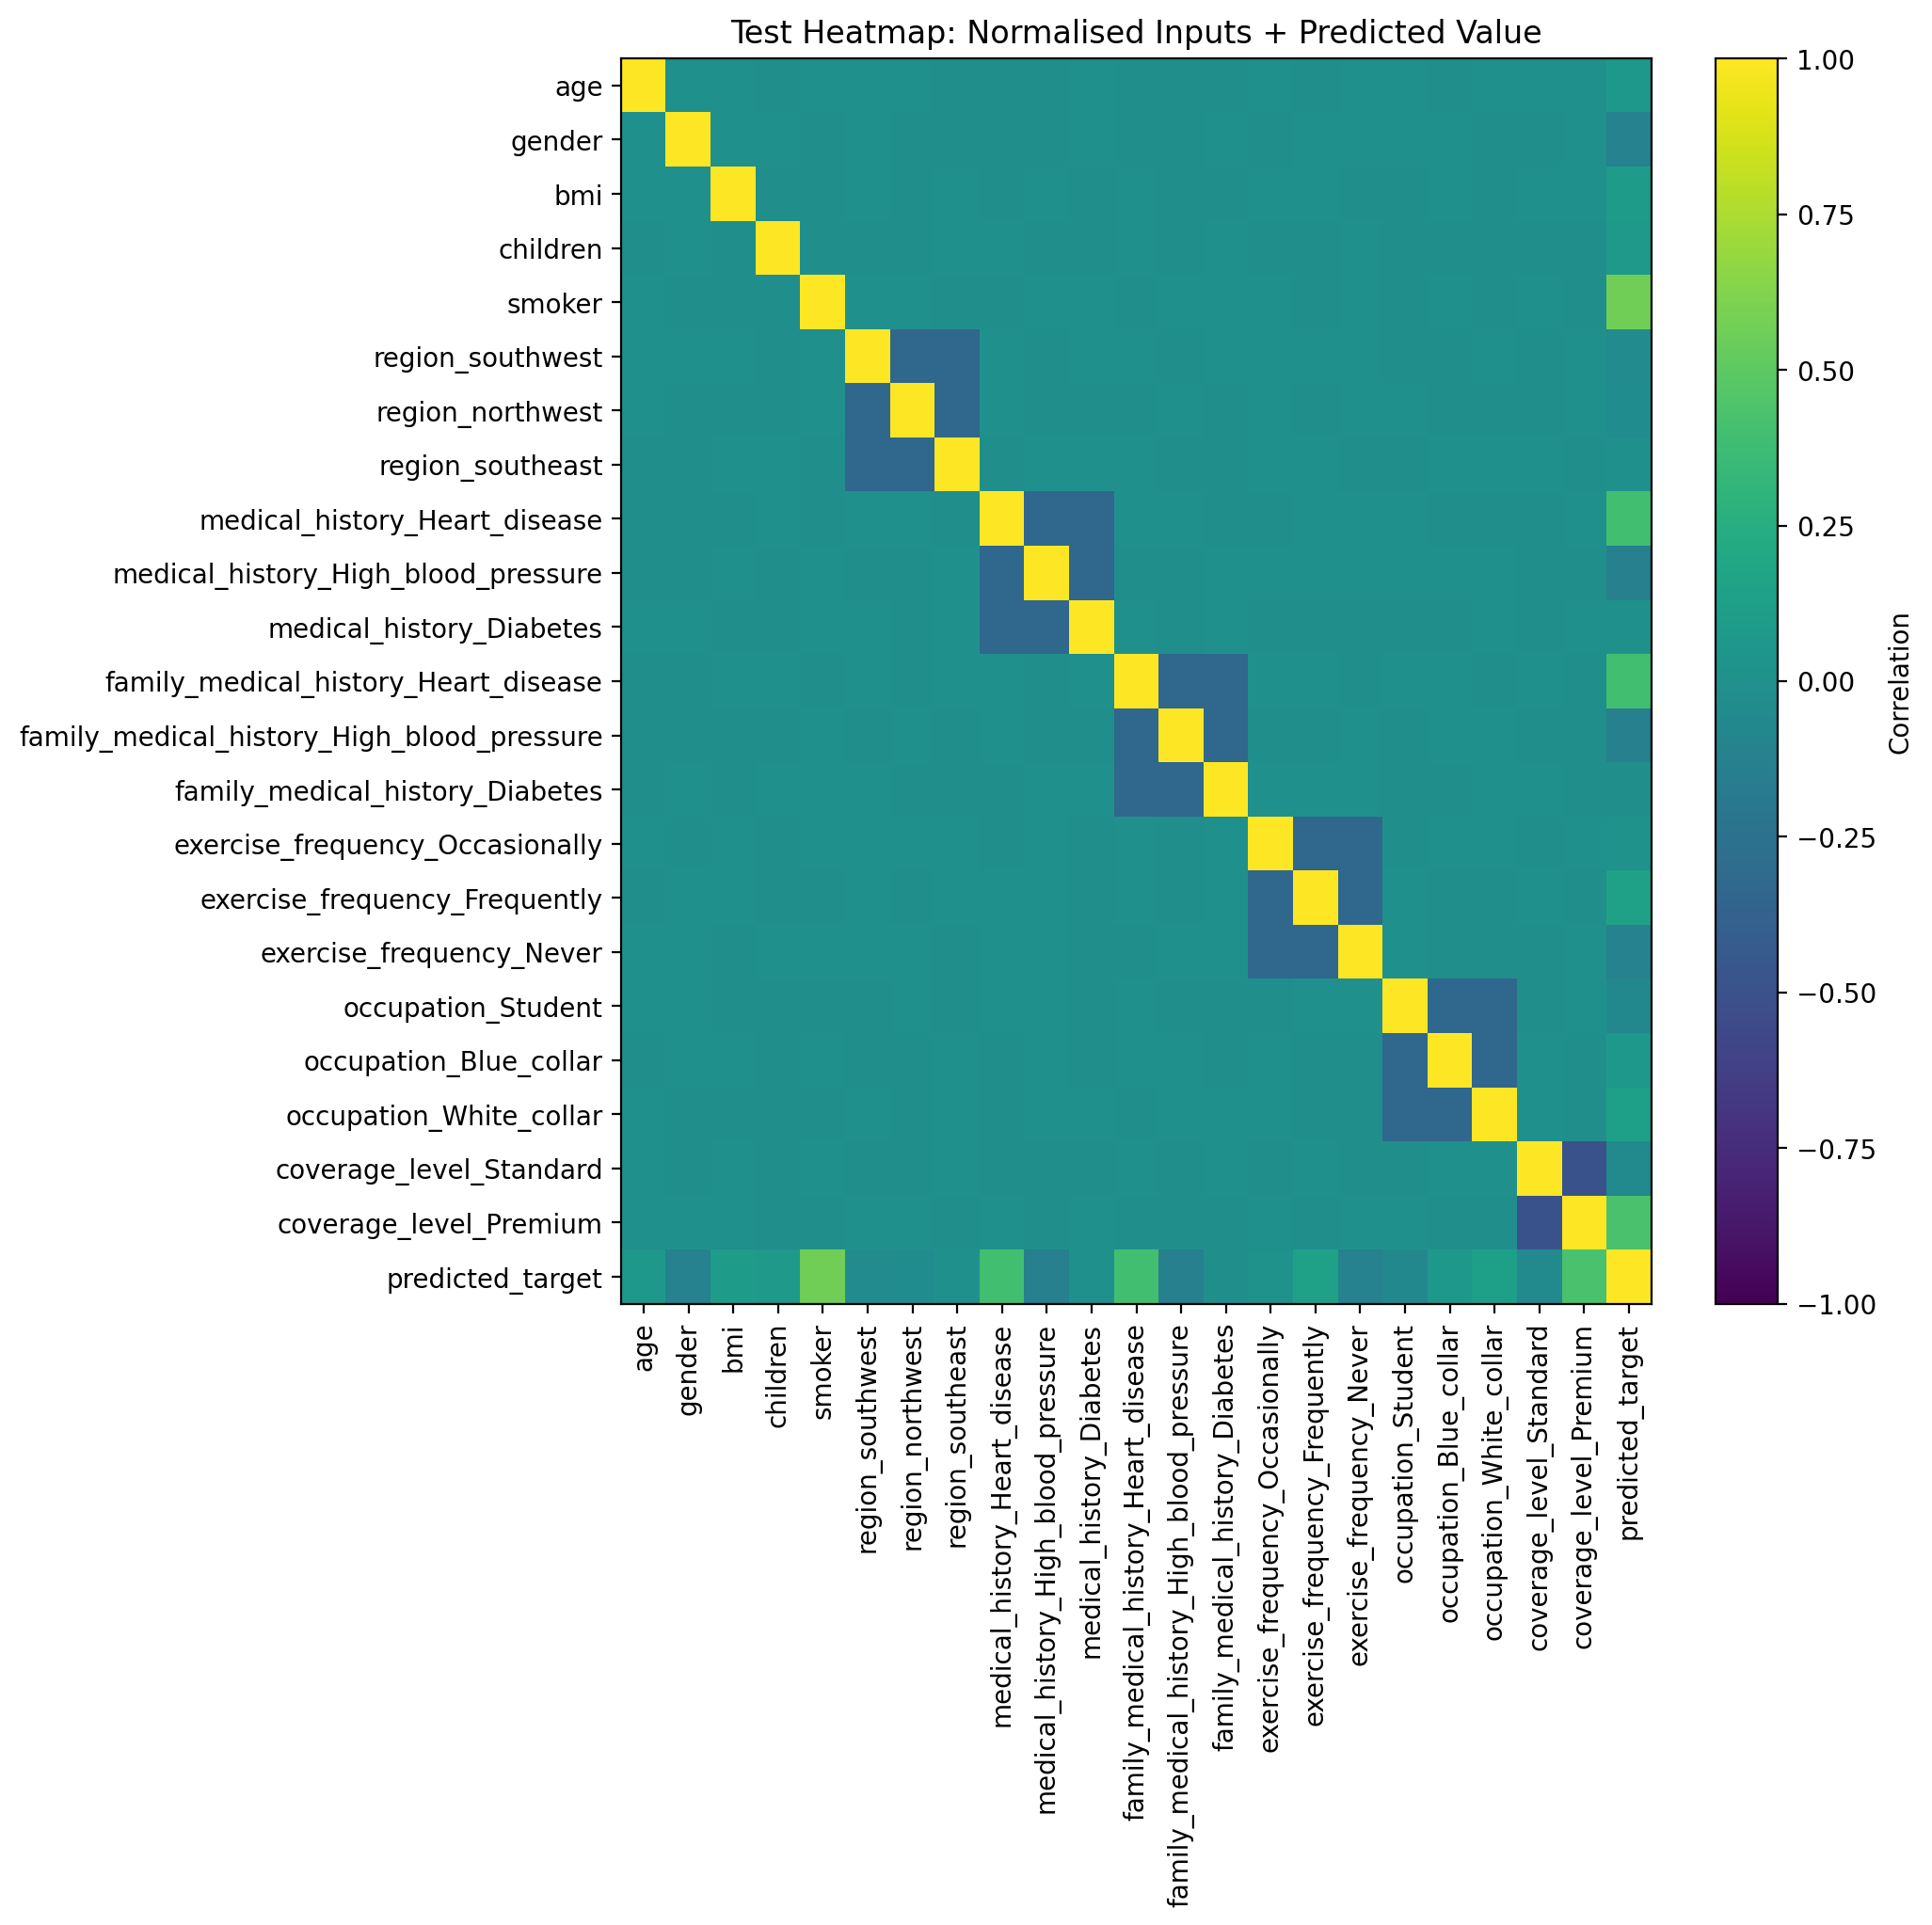
\includegraphics[width=\textwidth]{Thesis/Chapter 3/Figures/fig_sml_heatmap_test_predicted.png}
    \caption{Test set, predicted charges.}
    \label{fig:heatmap_test_predicted_ch3}
\end{subfigure}
\caption{Input-target correlation heatmaps for actual and predicted charges.}
\label{fig:heatmap_diagnostics_ch3}
\end{figure}

\noindent
Figure~\ref{fig:heatmap_diagnostics_ch3} presents the four correlation
heatmaps. The inter-feature correlations are predominantly near zero (teal
shading), with the expected negative correlations visible within dummy
groups belonging to the same raw categorical variable (e.g.\ the
\texttt{medical\_\allowbreak{}history}, \texttt{region}, \texttt{occupation} and
\texttt{coverage\_\allowbreak{}level} dummy blocks). The bottom row of each panel shows
the feature-target correlations. In the training set
(Figure~\ref{fig:heatmap_train_actual_ch3}), \texttt{smoker} shows the
largest positive correlation with actual charges (bright green-yellow),
followed by \texttt{coverage\_level\_\allowbreak{}Premium},
\texttt{medical\_history\_\allowbreak{}Heart\_disease} and \texttt{bmi}. The predicted
version (Figure~\ref{fig:heatmap_train_predicted_ch3}) displays a virtually
identical target row, confirming that the fitted \gls{dnn} has preserved the
linear association structure. The test set
(Figures~\ref{fig:heatmap_test_actual_ch3}
and~\ref{fig:heatmap_test_predicted_ch3}) reproduces the same patterns,
with the target-correlation rows near-identical across both the actual and
predicted versions. These consistency findings complete the diagnostic
verification; the fitted \gls{dnn} is therefore ready to serve as the prediction
surface for the \gls{mc} and Shapley-value analyses that follow.


% =============================================================
\subsection{Parametric MC Simulation Design}
\label{sec:mc_simulation_design}

The \gls{mc} stage generates a synthetic policyholder input space and
the corresponding model-implied distribution of predicted costs.  Each raw
predictor variable is assigned a fitted simulation distribution, synthetic
policyholder profiles are drawn from these distributions, and the fitted
\gls{dnn} computes predicted costs for the generated profiles.  The
simulation is performed at the raw-variable level: categorical variables
are simulated as valid categories first and are only then transformed into
the same encoding used during model training.  Dummy variables are never
simulated independently, since that could produce impossible category
combinations.

\subsubsection{Joint input distribution}

The joint simulation distribution is constructed as a product of fitted
marginal distributions, following the principle of
equation~\eqref{eq:input_law}.  Let
$\mathbf{X}_{\mathrm{raw}} = (X_1, X_2, \ldots, X_q)$ denote the vector of
raw predictor variables, where $q = 11$.  Applying the product-marginal
construction of equation~\eqref{eq:input_law} to the raw variables before
encoding yields
\begin{equation}
    \widehat{F}_{X,\mathrm{raw}}
    =
    \prod_{j=1}^{q}
    \widehat{F}_{X_j}.
    \label{eq:raw_product_mc_distribution_ch3}
\end{equation}
\equationlistentry{Product-marginal \gls{mc} input distribution}
As discussed in Section~\ref{montecarlo_propagation}, the product-marginal
construction is a modelling choice adopted for simulation purposes.  Two
empirical findings from the exploratory analysis support it in this dataset: the weak pairwise
correlations among the numerical predictors reported in
Table~\ref{tab:numeric_correlations}, and the observation that
\texttt{age}, \texttt{bmi}, and \texttt{children} are closely consistent
with independent uniform draws over their observed ranges
(Section~\ref{sec:eda_model_simulation_design}).  The product-marginal
construction is therefore not merely a computational convenience but a
faithful reflection of the benchmark data's apparent generating design.

\subsubsection{Fitted marginal distributions}

The fitted marginal distributions are selected using the empirical summaries
from the exploratory diagnostics.  All distributional parameters, including
the support bounds for the uniform distributions, are estimated from
$\mathcal{D}_{\mathrm{train}}$ only, ensuring that no validation- or
test-set information enters the simulation design.  Bounded numerical
variables are assigned distributions that respect their observed support.
Binary variables are generated from Bernoulli distributions.  Multi-level
categorical variables are generated using the observed training-set
proportions.  Table~\ref{tab:mc_distribution_assumptions_ch3} specifies the
distributional assumptions for each raw variable.

\begin{table}[H]
\centering
\small
\renewcommand{\arraystretch}{1.18}
\begin{tabular}{p{0.20\textwidth}p{0.16\textwidth}p{0.22\textwidth}p{0.20\textwidth}p{0.14\textwidth}}
\toprule
\textbf{Variable} &
\textbf{Type} &
\textbf{Distribution used} &
\textbf{Parameter estimation} &
\textbf{Support} \\
\midrule
\texttt{age} &
Bounded integer &
Discrete uniform &
$\widehat{a}=18,\ \widehat{b}=65$ &
$\{18,\ldots,65\}$ \\
\texttt{bmi} &
Bounded continuous &
Continuous uniform &
$\widehat{a}=18,\ \widehat{b}=50$ &
$[18,50]$ \\
\texttt{children} &
Bounded count &
Discrete uniform &
$\widehat{a}=0,\ \widehat{b}=5$ &
$\{0,\ldots,5\}$ \\
\texttt{gender} &
Binary &
Bernoulli &
$\widehat{p}_{\mathrm{male}} = n_{\mathrm{male}}/n_{\mathrm{train}}$ &
$\{0,1\}$ \\
\texttt{smoker} &
Binary &
Bernoulli &
$\widehat{p}_{\mathrm{yes}} = n_{\mathrm{yes}}/n_{\mathrm{train}}$ &
$\{0,1\}$ \\
\texttt{region} &
Categorical &
Categorical &
$\widehat{p}_{k}=n_k/n_{\mathrm{train}}$ &
Valid regions \\
\texttt{medical\_\allowbreak{}history} &
Categorical &
Categorical &
$\widehat{p}_{k}=n_k/n_{\mathrm{train}}$ &
Valid categories \\
\texttt{family\_medical\_\allowbreak{}history} &
Categorical &
Categorical &
$\widehat{p}_{k}=n_k/n_{\mathrm{train}}$ &
Valid categories \\
\texttt{exercise\_\allowbreak{}frequency} &
Categorical &
Categorical &
$\widehat{p}_{k}=n_k/n_{\mathrm{train}}$ &
Valid categories \\
\texttt{occupation} &
Categorical &
Categorical &
$\widehat{p}_{k}=n_k/n_{\mathrm{train}}$ &
Valid categories \\
\texttt{coverage\_\allowbreak{}level} &
Categorical &
Categorical &
$\widehat{p}_{k}=n_k/n_{\mathrm{train}}$ &
Valid tiers \\
\bottomrule
\end{tabular}
\caption{\gls{mc} input distributions for raw policyholder variables.}
\label{tab:mc_distribution_assumptions_ch3}
\end{table}

The fitted probabilities for categorical variables are estimated from the
training partition only, following the marginal parametric approach in
equation~\eqref{eq:mle_marginal}.  If $C$ is a categorical variable with
levels $c_1,\ldots,c_K$, then
\begin{equation}
    \widehat{p}_{k}
    =
    \frac{1}{n_{\mathrm{train}}}
    \sum_{i \in \mathcal{D}_{\mathrm{train}}}
    \mathbb{I}\{C_i = c_k\},
    \qquad
    k=1,\ldots,K.
    \label{eq:categorical_probability_estimator_ch3}
\end{equation}
\equationlistentry{Categorical probability estimator from training data}
A simulated categorical value is drawn as
$C^{(b)} \sim \operatorname{Categorical}(\widehat{p}_1,\ldots,\widehat{p}_K)$
and subsequently encoded using the reference-category scheme.

\subsubsection{Goodness-of-fit and support checks}

For continuous variables, empirical histograms and density overlays are
inspected, and Kolmogorov-Smirnov (K-S) and Anderson-Darling (A-D)
statistics are recorded.  These two statistics summarise complementary
aspects of marginal fit: the K-S statistic measures the maximum
absolute deviation between the empirical and fitted cumulative distribution
functions, while the A-D statistic places greater weight on the tails,
making it particularly sensitive to distributional departures in the regions
most relevant to the high-cost analysis.  Because the parameters of the
fitted marginals are estimated from the training data, the standard
critical values of these tests are invalid (the Lilliefors problem); the
K-S and A-D statistics are therefore reported as descriptive distance
measures of marginal fit rather than as formal hypothesis tests with
nominal critical values or $p$-values.  Parametric-bootstrap calibration
would be required to obtain valid $p$-values, and is not pursued because
the statistics serve a purely descriptive role here.  For the discrete and
categorical variables (including \texttt{age} and \texttt{children}, to
which continuous-distribution K-S theory does not apply), the comparison
is instead made between the empirical and fitted probability mass
functions, using frequency tables and chi-squared discrepancy summaries
interpreted in the same descriptive spirit.  Because the sample size is
large, even negligibly small distributional differences would be flagged
as significant by formal tests without being practically important for
simulation, which further motivates the descriptive treatment.  Support
restrictions are treated as compulsory: simulated numerical predictors are
confined to their observed ranges and categorical variables take only valid
observed levels.

\subsubsection{Sample size and convergence monitoring}

The base simulation uses $B = 100\,000$ generated policyholder profiles.  A
pilot convergence check is conducted by repeating the simulation for
increasing values of $B \in \{1\,000,\ 2\,500,\ 5\,000,\ 10\,000,\
25\,000,\ 50\,000,\ 100\,000\}$.  For each $B$, the running mean, standard deviation, and
selected quantiles of the simulated predicted costs are recorded.  The Monte
Carlo standard error is estimated using equation~\eqref{eq:mcse}, with
$s_B$ denoting the simulated standard deviation.  This mean-based
\gls{mcse} formula does not apply to quantiles: for a quantile level
$u \in (0,1)$, the Monte Carlo uncertainty is instead governed by the
asymptotic variance
$u(1-u)/\bigl(B\,f\bigl(F^{-1}(u)\bigr)^{2}\bigr)$, where $f$ denotes the
density of the predicted-cost distribution at the quantile of interest;
percentile stability is therefore assessed descriptively across the
increasing pilot sizes.  The selected simulation
size is retained when running summaries are stable relative to the scale of
the response variable.

\begin{table}[H]
\centering
\small
\renewcommand{\arraystretch}{1.15}
\begin{tabular}{p{0.25\textwidth}p{0.60\textwidth}}
\toprule
\textbf{Quantity} & \textbf{Purpose} \\
\midrule
Running mean & Checks stability of the average simulated predicted cost \\
Running standard deviation & Checks stability of simulated output spread \\
Median & Checks central distributional stability \\
90th percentile & Checks upper-tail stability \\
95th percentile & Candidate high-cost threshold \\
99th percentile & Extreme upper-tail stability check \\
\gls{mcse} & Quantifies simulation precision for selected summaries \\
\bottomrule
\end{tabular}
\caption{\gls{mc} convergence quantities recorded during the pilot run.}
\label{tab:mc_convergence_quantities_ch3}
\end{table}

\subsubsection{Base DNN MC scoring}

For each simulated raw profile, the preprocessing map $T(\cdot)$ produces
the model-ready input vector $\mathbf{z}^{(b)}$.  The fitted \gls{dnn} then
calculates the base \gls{mc} prediction, following the formulation in
equation~\eqref{eq:mc_predictions_framework}:
\begin{equation}
    \widehat{Y}^{(b)}
    =
    \widehat{m}
    \left(
        \mathbf{z}^{(b)}
    \right),
    \qquad
    b=1,\ldots,B.
    \label{eq:base_mc_prediction_ch3}
\end{equation}
\equationlistentry{Base \gls{mc} \gls{dnn} prediction}
The resulting collection
$\{\widehat{Y}^{(1)},\ldots,\widehat{Y}^{(B)}\}$
forms the base model-implied predicted-cost distribution introduced in
equation~\eqref{eq:mc_predictions_framework}.  The generated input profiles are also summarised
before interpreting the predicted-cost outputs, to confirm what type of
simulated input space produced the \gls{dnn} predictions.

\begin{table}[H]
\centering
\small
\renewcommand{\arraystretch}{1.15}
\begin{tabular}{p{0.92\textwidth}}
\toprule
\textbf{Algorithm 3.1: Base parametric \gls{mc} simulation} \\
\midrule
\textbf{Input:} fitted raw-variable distributions
$\{\widehat{F}_{X_j}\}_{j=1}^{q}$, fitted model
$\widehat{m}(\cdot)$, preprocessing map $T(\cdot)$, number of
replications $B$, random seed $s$. \\[3pt]

\textbf{Output:} simulated raw profiles
$\{\mathbf{X}_{\mathrm{raw}}^{(b)}\}_{b=1}^{B}$, model-ready profiles
$\{\mathbf{z}^{(b)}\}_{b=1}^{B}$, and base predicted costs
$\{\widehat{Y}^{(b)}\}_{b=1}^{B}$. \\[3pt]

1. Set the random seed to $s$. \\
2. For $b=1,\ldots,B$, simulate each raw variable from its fitted marginal distribution. \\
3. For categorical variables, simulate a valid category before applying reference-category encoding. \\
4. Apply the training-set preprocessing map $T(\cdot)$ to obtain $\mathbf{z}^{(b)}$. \\
5. Calculate $\widehat{Y}^{(b)} = \widehat{m}(\mathbf{z}^{(b)})$. \\
6. Transform predictions back to the original monetary scale if the network output is on the standardised scale. \\
7. Store the simulated inputs, encoded inputs and predicted costs. \\
\bottomrule
\end{tabular}
\caption{Base \gls{mc} simulation algorithm.}
\label{tab:base_mc_algorithm_ch3}
\end{table}

% =============================================================
\subsection{Validation of the MC Input Distribution}
\label{sec:mc_input_validation}

The product-marginal simulation law in
equation~\eqref{eq:raw_product_mc_distribution_ch3} constructs the joint
input distribution as a product of independent fitted marginals. Even if
every marginal distribution matches the training data closely, the joint
distribution of the simulated profiles is structurally different from the
joint distribution of the training data because all cross-variable
dependencies are set to zero by construction. This section diagnoses the
magnitude of that joint-distribution difference and then assesses whether it
affects the Shapley-value attributions derived from the simulated profiles.

\subsubsection{Joint distribution diagnostics}

The first diagnostic examines the difference between correlation
matrices.  Because Pearson correlation is undefined for unordered nominal
variables such as \texttt{region}, \texttt{occupation} and
\texttt{medical\_\allowbreak{}history}, this comparison is carried out on
the model-ready encoded representation, in which the numerical variables
enter directly and each categorical variable enters through its binary
dummy indicators.  The Pearson correlation matrix of the encoded columns
is computed separately on the training partition and on the parametric
\gls{mc} sample. The element-wise difference
\begin{equation}
    \Delta_{jk}
    =
    r_{jk}^{(\mathrm{train})}
    -
    r_{jk}^{(\mathrm{MC})},
    \qquad
    j,k = 1,\ldots,p,
    \label{eq:correlation_difference_ch3}
\end{equation}
\equationlistentry{Correlation matrix difference (training minus \gls{mc})}
quantifies how the pairwise linear association structure of the simulated
profiles deviates from that of the training data. Because the parametric
\gls{mc} sample draws each raw variable independently, the correlations
between encoded columns derived from different raw variables are
approximately zero by construction (the mechanical negative correlations
within a dummy group arise in both datasets), so
$\Delta_{jk} \approx r_{jk}^{(\mathrm{train})}$ for column pairs from
different raw variables. The resulting difference heatmap therefore
reveals which variable pairs carry the strongest dependencies in the
training data that are absent from the simulation.  Linear correlation on
binary indicators is a limited measure of association for nominal
attributes, so this diagnostic is complemented by the Cram\'{e}r's $V$
comparison below, which measures categorical association directly.

\begin{figure}[H]
\centering
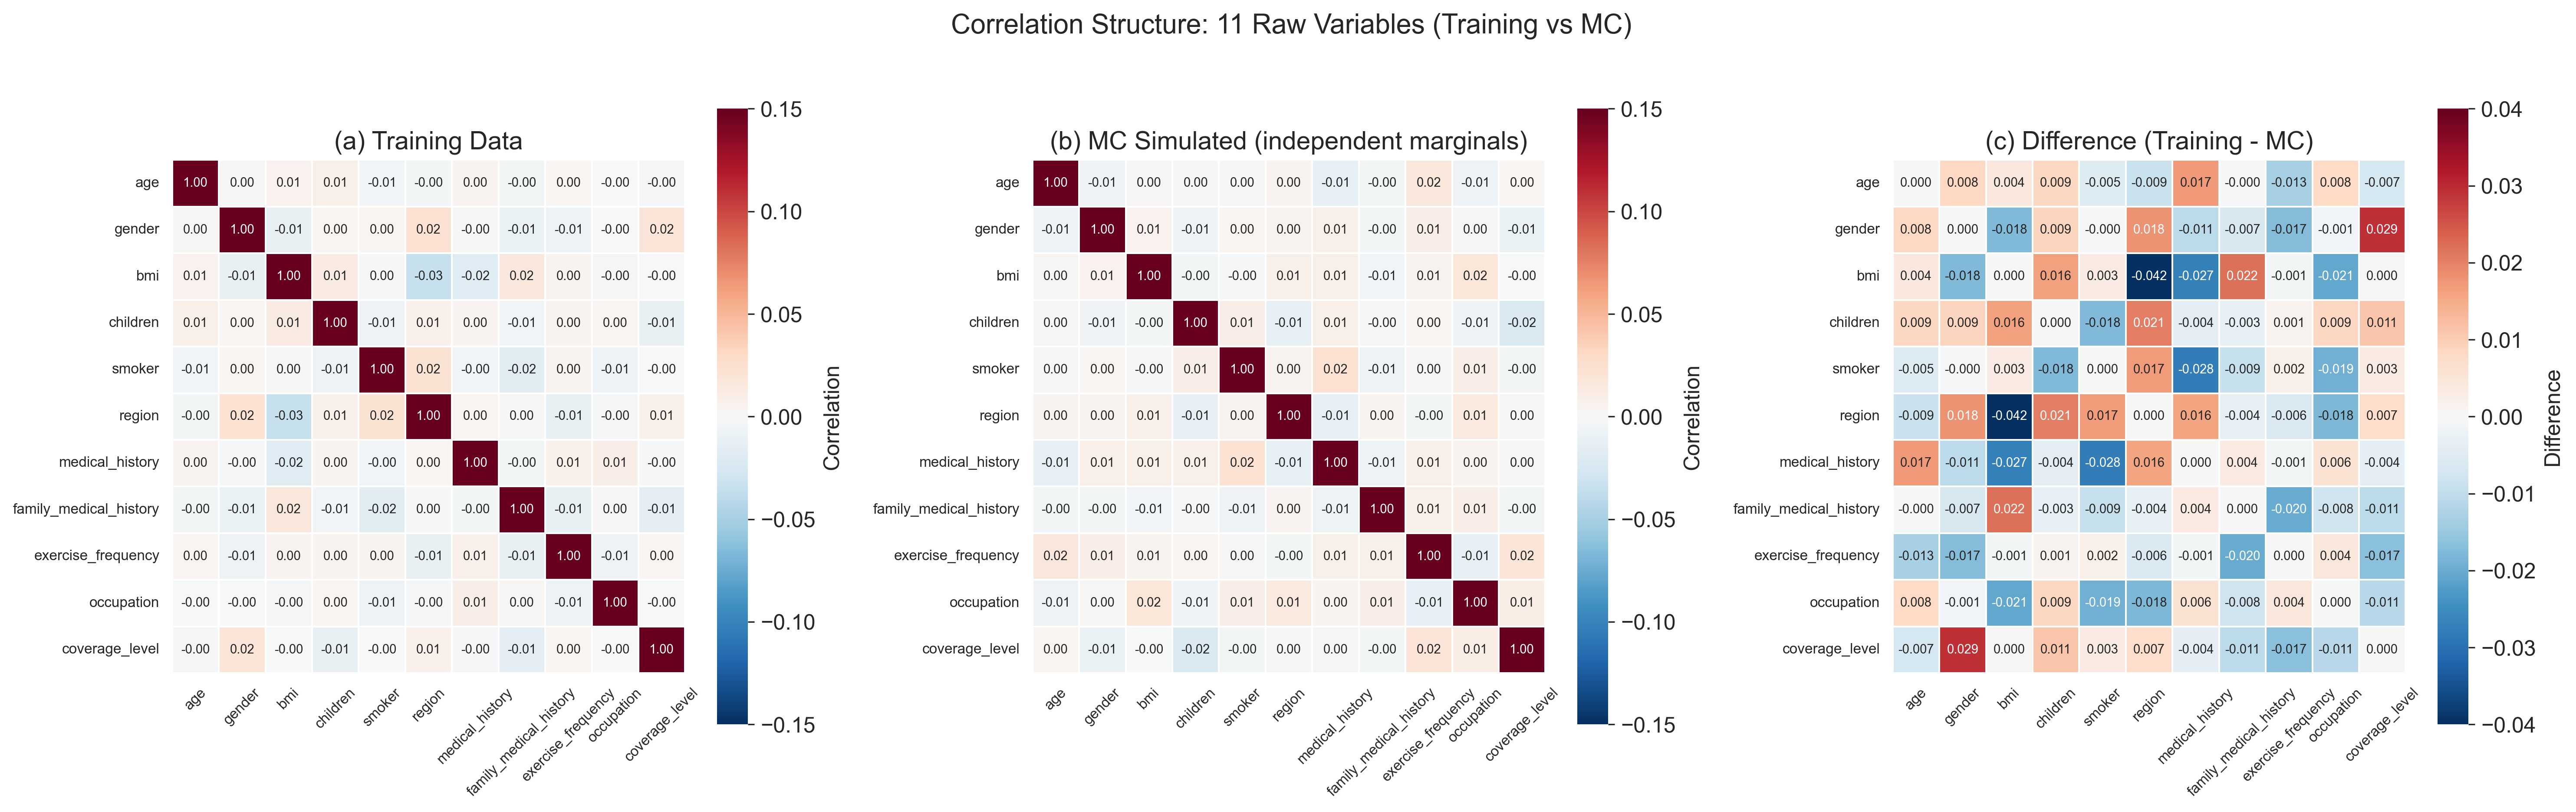
\includegraphics[width=0.90\textwidth]{Thesis/Chapter 3/Figures/fig_mc_joint_correlation_comparison.png}
\caption{Correlation structure comparison: training data versus parametric \gls{mc} sample.}
\label{fig:correlation_difference_heatmap_ch3}
\end{figure}

The second diagnostic addresses the categorical predictors.  For
multi-level categorical predictors the strength of pairwise association is
measured using Cram\'{e}r's $V$ statistic \citep{cramer1946mathematical}.
For each pair of categorical variables, $V$ is computed on the training
partition and on the parametric \gls{mc} sample. All pairwise values of
$V$ are compared to confirm that cross-variable associations are below a
weak-association threshold in both datasets and that the parametric \gls{mc}
sample, which has exactly zero association by construction, does not
materially differ from the training data.

\begin{figure}[H]
\centering
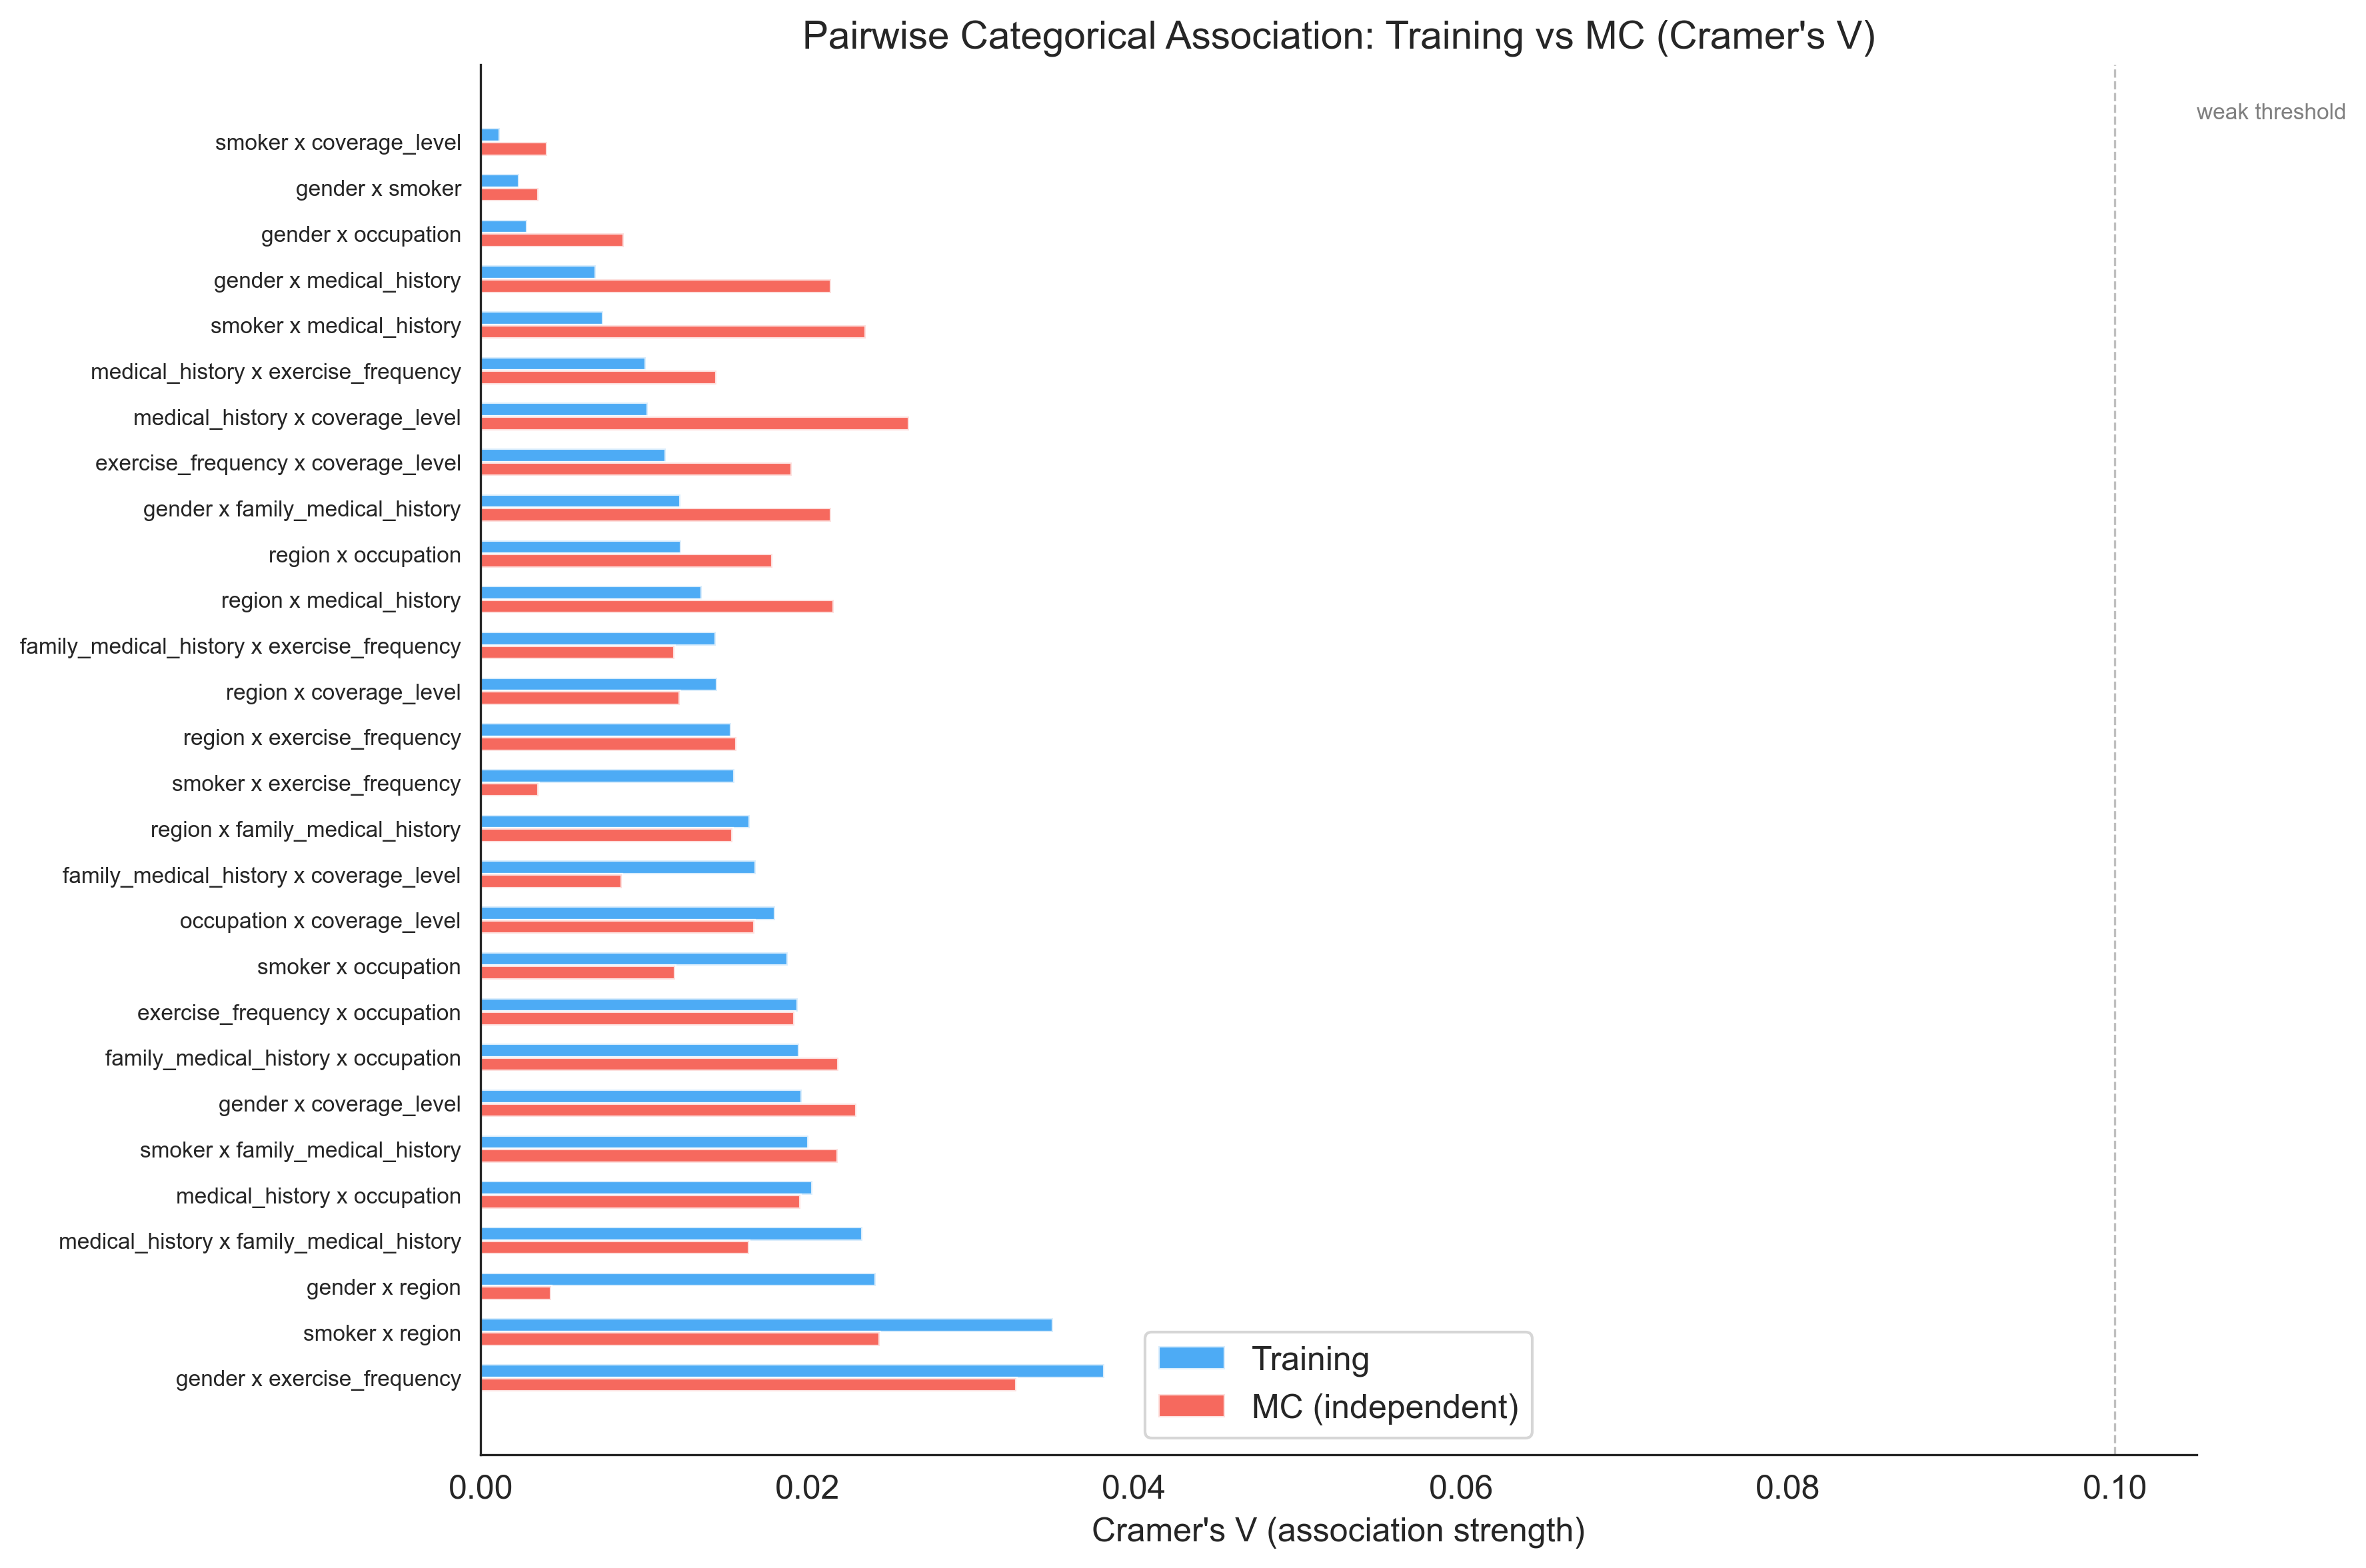
\includegraphics[width=0.90\textwidth]{Thesis/Chapter 3/Figures/fig_mc_joint_cramers_v.png}
\caption{Cram\'{e}r's $V$ comparison: training versus parametric \gls{mc} sample.}
\label{fig:cramers_v_comparison_ch3}
\end{figure}

The third diagnostic is a \gls{pca} overlay of the joint input space.
A principal component projection provides a visual comparison of the joint
input structure. The first two principal components are computed from the
standardised training inputs (using the eigenvectors from
Section~\ref{sec:pca_structural_diagnostics}), and both the training set
and the parametric \gls{mc} sample are projected onto these components. The two
point clouds are overlaid with distinct colours. If the independence
assumption substantially alters the joint structure, the \gls{mc} cloud will
appear more spread out or exhibit less internal clustering than the training
cloud. As reported in Section~\ref{sec:pca_structural_diagnostics}
(Figure~\ref{fig:pca_loadings_ch3}), the first two principal components are
dominated by the \texttt{coverage\_\allowbreak{}level} variable yet together
account for only about $13\%$ of total variance, so no single direction
dominates the 22-dimensional input space.

\begin{figure}[H]
\centering
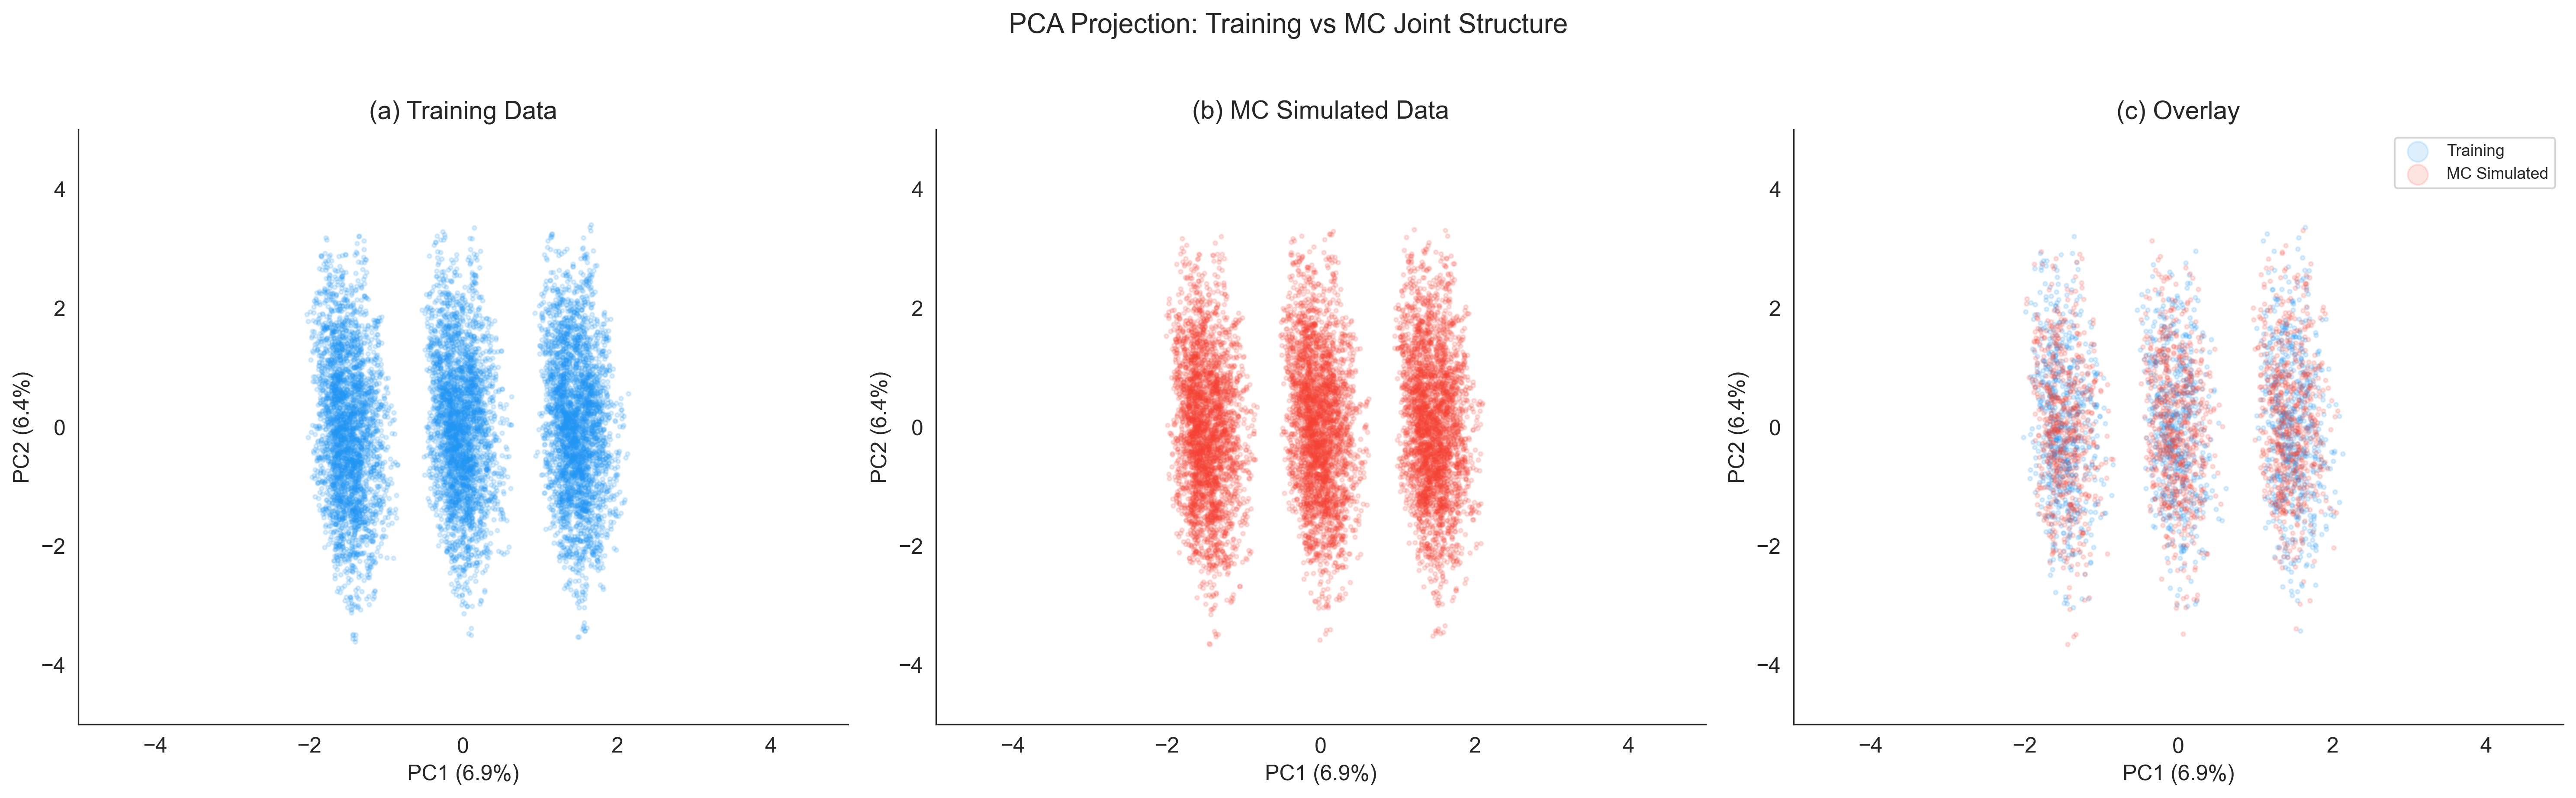
\includegraphics[width=0.95\textwidth]{Thesis/Chapter 3/Figures/fig_mc_joint_pca_comparison.png}
\caption{\Gls{pca} projection of joint input structure: training, \gls{mc} sample and overlay.}
\label{fig:pca_joint_overlay_ch3}
\end{figure}

\noindent
The \gls{mc} sample populates the same region of principal component
space as the training data. The vertical banding visible in both panels
reflects the discrete structure introduced by the categorical predictors.
The overlay in panel~(c) confirms that the two point clouds are broadly
co-located, with the \gls{mc} cloud exhibiting a marginally wider spread
consistent with the removal of the weak dependencies identified in the
correlation analysis.

\subsubsection{Bootstrap MC resampling}
\label{sec:bootstrap_mc_resampling}

To separate the effect of the independence assumption from the effect of
marginal distribution choice, a second \gls{mc} sample of size $B$ is
drawn via bootstrap resampling with replacement from the training set:
\begin{equation}
    \mathbf{X}_{\mathrm{raw}}^{(b,\mathrm{boot})}
    \sim
    \widehat{F}_{X,\mathrm{emp}},
    \qquad
    b = 1, \ldots, B,
    \label{eq:bootstrap_mc_ch3}
\end{equation}
\equationlistentry{Bootstrap \gls{mc} resampling from empirical distribution}
where $\widehat{F}_{X,\mathrm{emp}}$ is the empirical distribution of the
training data. This sample preserves the empirical joint distribution
exactly, including all cross-variable dependencies, while the parametric \gls{mc}
sample uses independent marginals. The bootstrap profiles are preprocessed
and scored through the fitted \gls{dnn} in the same manner as the
parametric profiles. Shapley values are then computed for both sets of
profiles using identical explainer settings, allowing a direct comparison of
the attribution results under the two input regimes.

\begin{table}[H]
\centering
\small
\renewcommand{\arraystretch}{1.15}
\begin{tabular}{p{0.24\textwidth}p{0.33\textwidth}p{0.33\textwidth}}
\toprule
\textbf{Property} & \textbf{Parametric \gls{mc}} & \textbf{Bootstrap \gls{mc}} \\
\midrule
Marginals &
Fitted parametric (uniform, Bernoulli, categorical) &
Empirical (training-set resampled) \\

Joint structure &
Independent (product of marginals) &
Empirical (preserves all dependencies) \\

Sample size &
$B = 100{,}000$ &
$B = 100{,}000$ \\

Purpose &
Primary simulation for cost distribution and Shapley analysis &
Validation check for Shapley invariance to input dependence \\
\bottomrule
\end{tabular}
\caption{Comparison of the two \gls{mc} input regimes.}
\label{tab:mc_input_regimes_ch3}
\end{table}

\subsubsection{Shapley invariance assessment}

The mean absolute Shapley values $I_g$ are aggregated to the raw-variable
level ($q = 11$ variables) and compared between the parametric \gls{mc} and
bootstrap \gls{mc} profiles. If the Shapley attributions are driven by the fitted
\gls{dnn}'s internal importance structure rather than by the particular
dependence pattern in the input profiles, the two sets of attributions
should be nearly identical.

The comparison is summarised by the Spearman rank correlation between the
two feature-importance vectors:
\begin{equation}
    \rho_{\mathrm{S}}
    =
    \operatorname{Spearman}
    \!\left(
        \{I_g^{(\mathrm{param})}\}_{g=1}^{q},\;
        \{I_g^{(\mathrm{boot})}\}_{g=1}^{q}
    \right).
    \label{eq:spearman_shapley_invariance_ch3}
\end{equation}
\equationlistentry{Spearman rank correlation for Shapley invariance}
A rank correlation close to one indicates that the feature-importance
ordering is preserved regardless of whether the input profiles carry
training-data dependencies or assume full independence.

\begin{figure}[H]
\centering
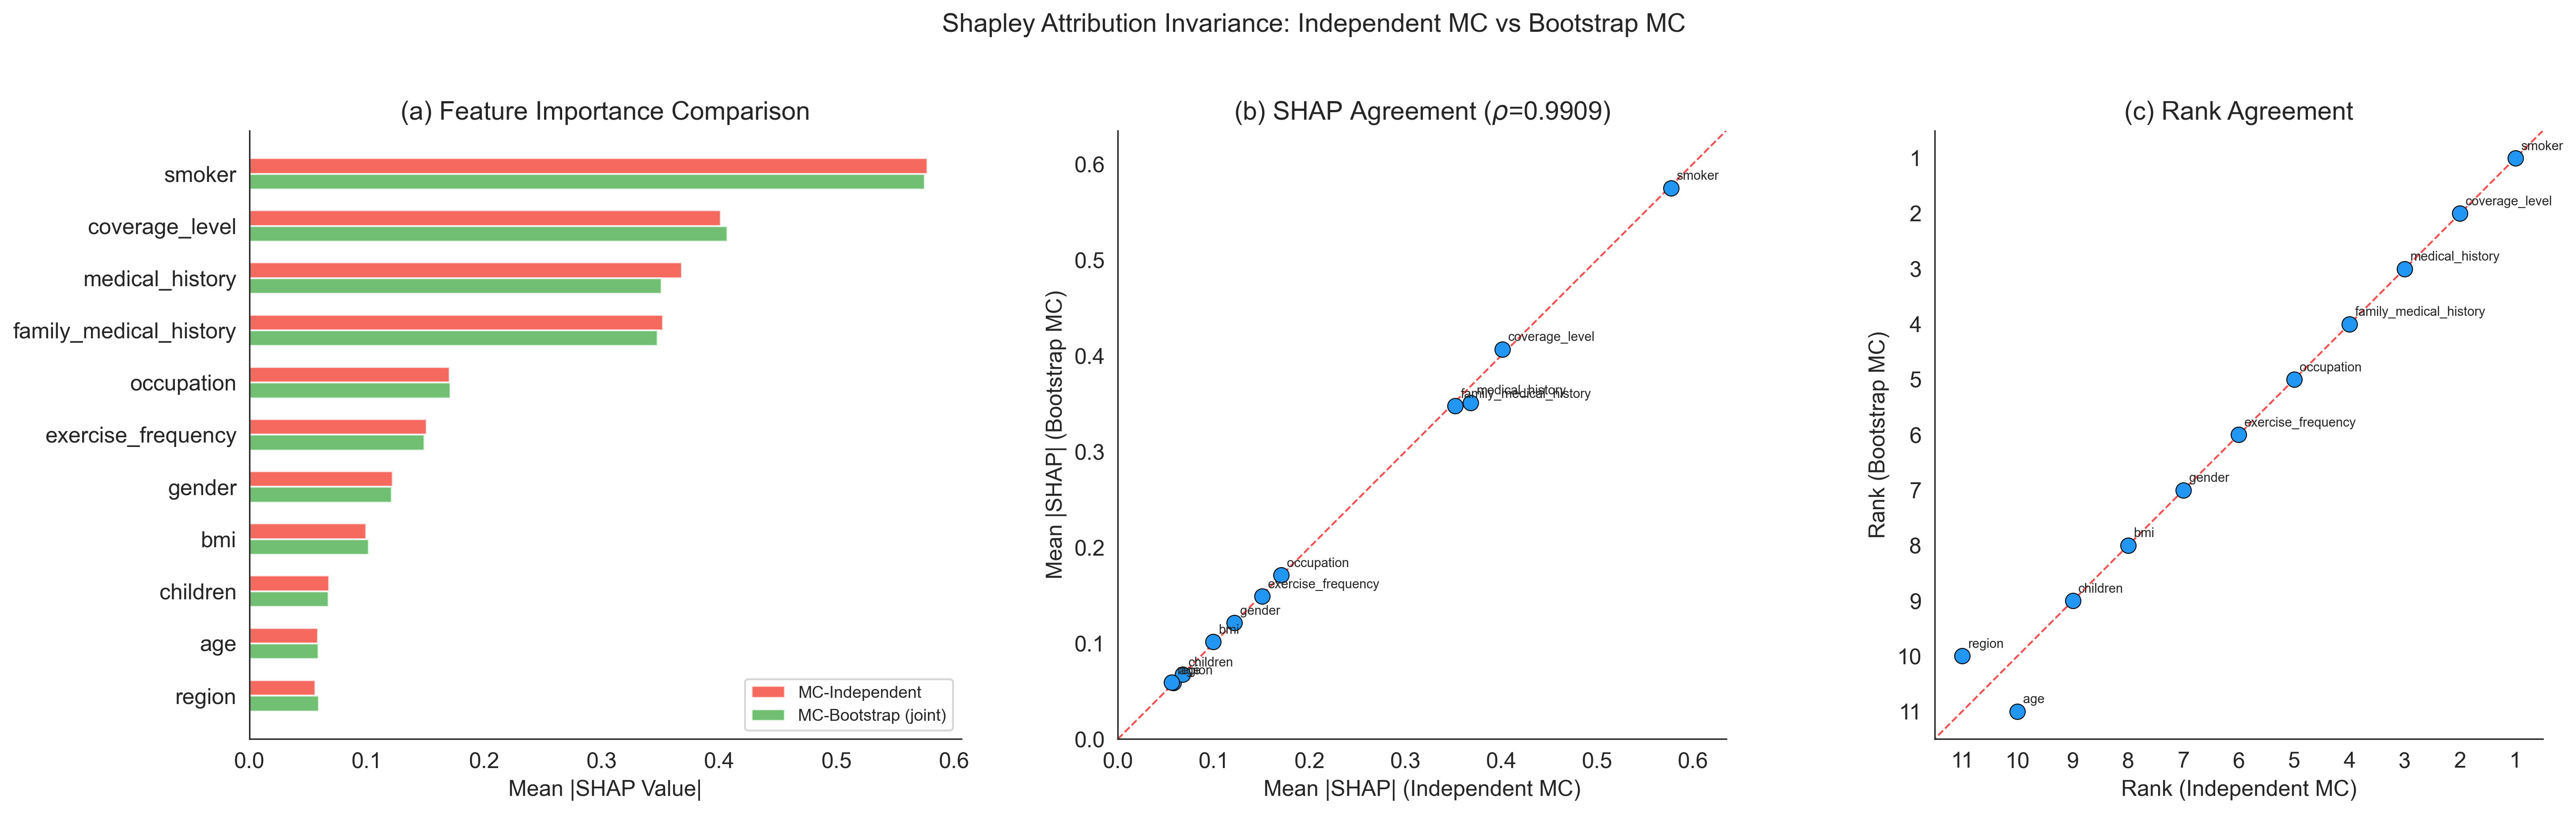
\includegraphics[width=0.95\textwidth]{Thesis/Chapter 3/Figures/fig_shap_bootstrap_vs_independent_invariance.png}
\caption{Shapley attribution invariance: parametric \gls{mc} versus bootstrap \gls{mc} input regimes.}
\label{fig:shapley_invariance_comparison_ch3}
\end{figure}

\subsubsection{Interpretation and conclusion}

The joint-distribution diagnostics confirm that the parametric \gls{mc} sample
differs from the training data in its dependence structure: the parametric
sample has zero cross-variable association by construction, whereas the
training data carries weak but non-zero dependencies. However, the
magnitude of these differences is small. The correlation matrix differences
do not exceed 0.042 (Figure~\ref{fig:correlation_difference_heatmap_ch3}),
all Cram\'{e}r's $V$ values fall below 0.04
(Figure~\ref{fig:cramers_v_comparison_ch3}), and the \gls{pca} overlays show that
both datasets populate the same region of principal component space
(Figure~\ref{fig:pca_joint_overlay_ch3}). The Shapley invariance comparison
yields a Spearman rank correlation of $\rho_{\mathrm{S}} = 0.991$ between
the parametric and bootstrap attribution vectors
(Figure~\ref{fig:shapley_invariance_comparison_ch3}), with the
feature-importance ordering preserved for all but the two weakest
contributors.

Because the joint-distribution differences are small and the Shapley
attributions are invariant to the input dependence structure, the
product-marginal independence assumption in
Section~\ref{sec:mc_simulation_design} is a defensible modelling choice. It
does not introduce meaningful bias into the subsequent high-cost conditional
Shapley analysis. The fitted \gls{dnn}'s internal importance structure,
rather than the dependence pattern of the input profiles, determines the
attribution results.

% =============================================================
\subsection{Residual-Augmented MC Sensitivity Analysis}
\label{sec:residual_augmented_mc}

A second \gls{mc} design assesses sensitivity to fitted residual
variation. The base \gls{mc} design produces deterministic fitted
predictions. The residual-augmented design adds a residual component to the
predicted costs to examine how the simulated output distribution changes
when fitted model error is introduced. The perturbation operates in the
output space (predicted costs) rather than the input space (policyholder
covariates). This is appropriate because the primary concern is whether the
distributional conclusions drawn from the base \gls{mc} analysis are
sensitive to the magnitude of the fitted model's residual error, not to
misspecification of the input distributions.

\subsubsection{Fitted residual distribution}

Let $e_i = y_i - \widehat{y}_i$ denote the fitted residual on the original
response scale for observations in the residual estimation set
$\mathcal{S}_{\varepsilon}$, taken as the training partition. Using the
training set for residual estimation is appropriate in this context because
the residuals serve only to characterise the magnitude and distributional
shape of fitted prediction error for the sensitivity analysis, not to assess
out-of-sample generalisation performance. The centred
residuals are
\begin{equation}
    e_i^{c}
    =
    e_i - \bar{e},
    \qquad
    \bar{e}
    =
    \frac{1}{|\mathcal{S}_{\varepsilon}|}
    \sum_{i \in \mathcal{S}_{\varepsilon}}
    e_i.
    \label{eq:centered_residuals_ch3}
\end{equation}
\equationlistentry{Centred fitted residuals}
The empirical residual distribution is
$\widehat{F}_{\varepsilon}
=
|\mathcal{S}_{\varepsilon}|^{-1}
\sum_{i \in \mathcal{S}_{\varepsilon}}
\delta_{e_i^{c}}$,
where $\delta_{e_i^{c}}$ denotes a point mass at $e_i^{c}$. The residual
standard deviation is
\begin{equation}
    \widehat{\sigma}_{\varepsilon}
    =
    \sqrt{
    \frac{1}{|\mathcal{S}_{\varepsilon}|-1}
    \sum_{i \in \mathcal{S}_{\varepsilon}}
    \left(
        e_i - \bar{e}
    \right)^2
    }.
    \label{eq:residual_sd_ch3}
\end{equation}
\equationlistentry{Residual standard deviation}

\subsubsection{Residual-augmented simulation}

For each base \gls{mc} prediction $\widehat{Y}^{(b)}$, a residual draw is
sampled:
\begin{equation}
    \varepsilon^{(b)}
    \sim
    \widehat{F}_{\varepsilon},
    \qquad
    b=1,\ldots,B.
    \label{eq:residual_draw_ch3}
\end{equation}
\equationlistentry{Residual draw from empirical distribution}
The residual-augmented predicted cost is
\begin{equation}
    Y_{\mathrm{res}}^{(b)}
    =
    \widehat{Y}^{(b)}
    +
    \varepsilon^{(b)},
    \qquad
    b=1,\ldots,B.
    \label{eq:residual_augmented_prediction_ch3}
\end{equation}
\equationlistentry{Residual-augmented predicted cost}
Negative values are truncated at zero:
$Y_{\mathrm{res},+}^{(b)}
=
\max\{0,\, Y_{\mathrm{res}}^{(b)}\}$.

\subsubsection{Fixed residual perturbation check}

A fixed perturbation check assesses sensitivity to the magnitude of residual
augmentation:
\begin{equation}
    Y_{+}^{(b)}
    =
    \widehat{Y}^{(b)}
    +
    0.5\,\widehat{\sigma}_{\varepsilon},
    \qquad
    Y_{-}^{(b)}
    =
    \max
    \left\{
        0,\,
        \widehat{Y}^{(b)}
        -
        0.5\,\widehat{\sigma}_{\varepsilon}
    \right\}.
    \label{eq:fixed_residual_perturbation_ch3}
\end{equation}
\equationlistentry{Fixed residual perturbation sensitivity band}
This is a deterministic sensitivity band around the fitted \gls{dnn} predictions,
not a probabilistic uncertainty interval. The residual-augmented simulation is
interpreted as a sensitivity analysis based on fitted residual variability. It
does not account for parameter uncertainty, model uncertainty or
data-generating uncertainty.

\begin{table}[H]
\centering
\small
\renewcommand{\arraystretch}{1.15}
\begin{tabular}{p{0.32\textwidth}p{0.58\textwidth}}
\toprule
\textbf{Component} & \textbf{Specification} \\
\midrule
Base prediction & $\widehat{Y}^{(b)} = \widehat{m}(\mathbf{z}^{(b)})$ \\
Residual source & Fitted residuals from the training partition \\
Residual centring & Residuals centred before resampling \\
Main residual design & $\varepsilon^{(b)} \sim \widehat{F}_{\varepsilon}$ \\
Residual-augmented output & $Y_{\mathrm{res}}^{(b)} = \widehat{Y}^{(b)}+\varepsilon^{(b)}$ \\
Fixed perturbation check & $\widehat{Y}^{(b)} \pm 0.5\,\widehat{\sigma}_{\varepsilon}$ \\
Non-negativity rule & Negative simulated costs truncated at zero \\
\bottomrule
\end{tabular}
\caption{Residual-augmented \gls{mc} sensitivity design.}
\label{tab:residual_augmented_design_ch3}
\end{table}

\begin{table}[H]
\centering
\small
\renewcommand{\arraystretch}{1.15}
\begin{tabular}{p{0.92\textwidth}}
\toprule
\textbf{Algorithm 3.2: Residual-augmented \gls{mc} sensitivity simulation} \\
\midrule
\textbf{Input:} base \gls{mc} predictions
$\{\widehat{Y}^{(b)}\}_{b=1}^{B}$, fitted residual distribution
$\widehat{F}_{\varepsilon}$, residual standard deviation
$\widehat{\sigma}_{\varepsilon}$, random seed $s$. \\[3pt]

\textbf{Output:} residual-augmented outputs
$\{Y_{\mathrm{res}}^{(b)}\}_{b=1}^{B}$, upper perturbation outputs
$\{Y_{+}^{(b)}\}_{b=1}^{B}$, and lower perturbation outputs
$\{Y_{-}^{(b)}\}_{b=1}^{B}$. \\[3pt]

1. Set the random seed to $s$. \\
2. Estimate residuals $e_i = y_i-\widehat{y}_i$ on the residual estimation set. \\
3. Centre the residuals and construct $\widehat{F}_{\varepsilon}$. \\
4. For $b=1,\ldots,B$, draw $\varepsilon^{(b)} \sim \widehat{F}_{\varepsilon}$. \\
5. Calculate $Y_{\mathrm{res}}^{(b)} = \widehat{Y}^{(b)}+\varepsilon^{(b)}$. \\
6. Apply the non-negativity rule if required. \\
7. Calculate the fixed perturbation outputs $Y_{+}^{(b)}$ and $Y_{-}^{(b)}$. \\
8. Store all outputs for comparison with the base \gls{mc} distribution. \\
\bottomrule
\end{tabular}
\caption{Residual-augmented \gls{mc} algorithm.}
\label{tab:residual_augmented_algorithm_ch3}
\end{table}


% =============================================================
\subsection{Shapley-Value Attribution for Simulated Profiles}
\label{sec:shapley_attribution_simulated_profiles}
\label{sec:shapley_interpretation_design}
\label{sec:high_cost_conditional_shapley}

Shapley-value methods are used to explain the fitted \gls{dnn} predictions
calculated for simulated policyholder profiles. The attribution analysis is
connected to the \gls{mc} predicted-cost distribution, with particular
attention to the upper tail.

\subsubsection{Prediction function and Shapley decomposition}

The prediction function supplied to \gls{shap} is the fitted \gls{dnn}
together with the response de-normalisation step. Shapley values are
therefore reported on the original monetary scale of \texttt{charges}. For a
simulated model-ready profile $\mathbf{z}^{(b)}$, the fitted prediction is
decomposed following equation~\eqref{eq:shapley_decomp}, with $p = 22$
encoded features. The baseline prediction $\phi_0$ and the feature-level
contributions $\phi_j(\mathbf{z}^{(b)})$ are defined exactly as in
Section~\ref{sec:explainability_shapley_shap}.

\subsubsection{Implementation settings}

The background data are sampled from the model-ready training partition. The
primary implementation uses a gradient-based \gls{shap} explainer for the
differentiable \gls{dnn}. A model-agnostic KernelSHAP calculation may be
applied to a small validation subset as a computational check if required.

The gradient-based \gls{shap} explainer computes
approximate Shapley values, not exact game-theoretic Shapley
values.  Exact computation requires evaluating the prediction function at
all $2^p$ feature subsets, which is computationally infeasible for $p = 22$
encoded features ($2^{22} = 4\,194\,304$ coalition evaluations per
profile).  The gradient-based approximation leverages the differentiability
of the fitted \gls{dnn} to estimate feature contributions efficiently, but
the resulting attributions are conditional on the background sample, the
explainer algorithm, and the fitted network parameters.  All reported
Shapley values should therefore be interpreted as model-specific,
approximate attributions rather than exact cooperative-game solutions.

\begin{table}[H]
\centering
\small
\renewcommand{\arraystretch}{1.15}
\begin{tabular}{p{0.32\textwidth}p{0.58\textwidth}}
\toprule
\textbf{Item} & \textbf{Specification} \\
\midrule
Prediction function & Fitted \gls{dnn} with response de-normalisation \\
Output scale & Original monetary scale of \texttt{charges} \\
Explainer & Gradient-based \gls{shap} explainer \\
Background data & Sample from the model-ready training partition \\
Background size & $m_0 = 200$ observations, selected as the largest size that maintains computational feasibility for the gradient-based explainer \\
Explained profiles & \gls{mc} simulated profiles $\mathbf{z}^{(b)}$ \\
Primary summaries & Mean signed and mean absolute Shapley values \\
Conditional summaries & Shapley summaries for upper-tail simulated profiles \\
Categorical treatment & Dummy-level attributions aggregated to raw-variable level \\
\bottomrule
\end{tabular}
\caption{\Gls{shap} implementation settings.}
\label{tab:shap_implementation_settings_ch3}
\end{table}

\subsubsection{Aggregation from encoded inputs to raw variables}

The fitted \gls{dnn} receives $p = 22$ encoded features, but some columns are
dummy variables derived from a single raw categorical predictor. If $G_g$
denotes the set of encoded columns associated with raw variable $g$, the
raw-variable Shapley contribution is
\begin{equation}
    \Phi_g
    \left(
        \mathbf{z}^{(b)}
    \right)
    =
    \sum_{j \in G_g}
    \phi_j
    \left(
        \mathbf{z}^{(b)}
    \right).
    \label{eq:raw_variable_shap_aggregation_ch3}
\end{equation}
\equationlistentry{Raw-variable Shapley aggregation from encoded inputs}
This aggregation prevents the interpretation from being fragmented across
several dummy columns belonging to the same original variable.

The four Shapley axioms that uniquely characterise the Shapley value
\citep{shapley1953value} were discussed in
Section~\ref{sec:explainability_shapley_shap}.  In the present context, the
efficiency, symmetry, dummy, and additivity properties ensure that the
aggregation from encoded features to raw variables is a linear
repartitioning that preserves the complete decomposition.  The raw-variable
contributions $\Phi_g$ therefore retain the same axiomatic guarantees as the
underlying feature-level values $\phi_j$, and the total prediction remains
fully decomposed into $q = 11$ raw-variable contributions without remainder.

\subsubsection{Global Shapley summaries}

Shapley values are computed for all $B$ simulated profiles generated in the
base \gls{mc} simulation, so $B_{\mathrm{shap}} = B$. Global feature
importance $I_j$ follows the mean absolute Shapley value defined in
Section~\ref{sec:explainability_shapley_shap}, computed over the simulated
profiles. A mean signed summary is also reported.
The mean signed Shapley contribution for feature $j$ is
\begin{equation}
    \overline{\phi}_{j}
    =
    \frac{1}{B_{\mathrm{shap}}}
    \sum_{b=1}^{B_{\mathrm{shap}}}
    \phi_j
    \left(
        \mathbf{z}^{(b)}
    \right),
    \label{eq:mean_signed_shap_ch3}
\end{equation}
\equationlistentry{Mean signed Shapley contribution}
and the mean absolute Shapley contribution is
\begin{equation}
    I_j
    =
    \frac{1}{B_{\mathrm{shap}}}
    \sum_{b=1}^{B_{\mathrm{shap}}}
    \left|
        \phi_j
        \left(
            \mathbf{z}^{(b)}
        \right)
    \right|.
    \label{eq:mean_absolute_shap_ch3}
\end{equation}
\equationlistentry{Mean absolute Shapley contribution (feature importance)}
The signed summary describes the average direction of the contribution; the
absolute summary measures average magnitude.

\subsubsection{High-cost region and conditional Shapley summaries}

The high-cost region is defined using the quantile-based threshold
$u_{\tau}$ from equation~\eqref{eq:high_cost_threshold} and the
high-cost set $\mathcal{H}_{\tau}$ from
equation~\eqref{eq:high_cost_set}, applied to the $B$ simulated profiles
with $\tau \in \{0.90, 0.95, 0.99\}$.
The 95th percentile is used as the main high-cost threshold because it
balances two competing requirements: it retains a sufficient number of
upper-tail profiles ($|H_{0.95}| = 0.05B$) for stable conditional Shapley
averages, while still isolating profiles that represent genuinely high
predicted costs. The 90th and 99th percentiles are retained as sensitivity
thresholds to assess whether the attribution patterns are robust to the
choice of cutoff. The conditional mean signed contribution
$\overline{\phi}_{j,\tau}$ and the conditional mean absolute contribution
$I_{j,\tau}$ are computed as in
equations~\eqref{eq:signed_shapley_high}
and~\eqref{eq:abs_shapley_high}, with the high-cost set
$\mathcal{H}_{\tau}$ replacing the generic conditioning set and the
summation taken over the $B$ simulated profiles. These conditional
summaries are also aggregated to the raw-variable level using
equation~\eqref{eq:raw_variable_shap_aggregation_ch3}.
Comparing $I_j$ with $I_{j,\tau}$ shows whether a feature is generally
important across all simulated profiles or specifically important in the
high-cost region. For the residual-augmented simulation, a separate high-cost
set can be defined using the residual-augmented outputs to examine whether the
profiles classified as high cost change when fitted residual variability is
introduced. Since the residual component is added after the fitted \gls{dnn}
prediction, Shapley values explain the fitted \gls{dnn} component
$\widehat{m}(\mathbf{z}^{(b)})$ rather than the residual addition.

\subsubsection{Bootstrap confidence intervals for conditional Shapley values}

At $\tau_{99}$ the conditioning set contains only $|\mathcal{H}_{0.99}| = 0.01B$ profiles, so the conditional mean absolute Shapley values are estimated from a small effective sample. To quantify estimation uncertainty, a nonparametric bootstrap is applied. Let $\boldsymbol{\Phi}_{\tau} \in \mathbb{R}^{|\mathcal{H}_{\tau}| \times q}$ denote the matrix of raw-variable Shapley values for profiles in $\mathcal{H}_{\tau}$. The bootstrap procedure is:

\begin{enumerate}
    \item Draw $R = 10\,000$ bootstrap resamples $\boldsymbol{\Phi}_{\tau}^{*(r)}$, each of size $|\mathcal{H}_{\tau}|$, with replacement from $\boldsymbol{\Phi}_{\tau}$.
    \item For each resample $r$, compute the mean absolute Shapley value for each variable:
    \[
        I_{j,\tau}^{*(r)} = \frac{1}{|\mathcal{H}_{\tau}|} \sum_{i=1}^{|\mathcal{H}_{\tau}|} \bigl|\phi_{ij}^{*(r)}\bigr|, \qquad j = 1, \ldots, q.
    \]
    \item The 95\% bootstrap confidence interval for $I_{j,\tau}$ is the interval $\bigl[I_{j,\tau}^{*(0.025)},\; I_{j,\tau}^{*(0.975)}\bigr]$, where $I_{j,\tau}^{*(\alpha)}$ is the $\alpha$-quantile of the bootstrap distribution $\{I_{j,\tau}^{*(1)}, \ldots, I_{j,\tau}^{*(R)}\}$.
\end{enumerate}

This percentile bootstrap is reported alongside the conditional importance values at $\tau_{99}$ in Chapter~\ref{sec:results}.

\begin{table}[H]
\centering
\small
\renewcommand{\arraystretch}{1.15}
\begin{tabular}{p{0.30\textwidth}p{0.60\textwidth}}
\toprule
\textbf{Summary} & \textbf{Purpose} \\
\midrule
Mean signed Shapley value & Average directional effect on fitted predictions \\
Mean absolute Shapley value & Average contribution magnitude across simulated profiles \\
Raw-variable aggregated Shapley value & Combines dummy-level attributions into original variables \\
High-cost conditional Shapley value & Identifies drivers of upper-tail predicted costs \\
Threshold comparison & Compares attribution at 90th, 95th and 99th percentiles \\
Base versus residual high-cost sets & Checks whether residual augmentation changes high-cost membership \\
\bottomrule
\end{tabular}
\caption{Shapley summaries calculated for simulated profiles.}
\label{tab:shap_summaries_ch3}
\end{table}


% =============================================================
\subsection{Modelling Assumptions}
\label{sec:modelling_assumptions}

The empirical framework depends on the modelling assumptions stated in
Table~\ref{tab:modelling_assumptions_ch3}. These assumptions define the
boundary of the empirical claims: the analysis can support statements about
how the fitted \gls{dnn} behaves on the benchmark dataset and under the stated Monte
Carlo input assumptions, but cannot, without external validation, support
causal claims about healthcare expenditure.

\begin{table}[H]
\centering
\small
\renewcommand{\arraystretch}{1.16}
\begin{tabular}{p{0.06\textwidth}p{0.25\textwidth}p{0.59\textwidth}}
\toprule
\textbf{No.} & \textbf{Assumption} & \textbf{Interpretation} \\
\midrule
A1 &
Benchmark data &
The dataset is a public benchmark and not a representative insurer portfolio \\

A2 &
Training-set preprocessing &
Encoding, numerical scaling and response scaling are estimated from the training set and applied unchanged elsewhere \\

A3 &
Bias-free \gls{dnn} &
The constrained architecture is assessed empirically through validation and test diagnostics \\

A4 &
No explicit regularisation &
Generalisation is assessed using validation behaviour, held-out performance and structural diagnostics \\

A5 &
Raw-variable \gls{mc} simulation &
Synthetic profiles are generated at the raw variable level and only then encoded \\

A6 &
Product-marginal input distribution &
The joint \gls{mc} input law is a practical simulation assumption and not a proof of covariate independence; validated by joint-distribution diagnostics and Shapley invariance comparison (Section~\ref{sec:mc_input_validation}) \\

A7 &
Joint-distribution validation &
The Shapley attributions are shown to be invariant to whether input profiles preserve training-data dependencies (bootstrap \gls{mc}) or assume full independence (parametric \gls{mc}) \\

A8 &
Base \gls{mc} interpretation &
The base simulated output distribution represents \gls{dnn} fitted predictions under the stated input assumptions, not realised healthcare costs \\

A9 &
Residual augmentation &
Residual-augmented simulation is a sensitivity analysis and not a complete predictive uncertainty model \\

A10 &
Shapley interpretation &
Shapley values explain the fitted \gls{dnn} predictions and are not causal feature effects \\

A11 &
High-cost definition &
High-cost profiles are defined by empirical upper-tail quantiles of the simulated predicted-cost distribution \\
\bottomrule
\end{tabular}
\caption{Summary of modelling assumptions and interpretive boundaries.}
\label{tab:modelling_assumptions_ch3}
\end{table}

With the data, architecture, simulation design, attribution method and
modelling assumptions now fully specified, the empirical results of the
three-stage framework are presented in Chapter~\ref{sec:results}.

